\documentclass[12pt,a4paper]{book}
%宏包
\usepackage{amsmath}
\usepackage{amssymb}
\usepackage{amsthm}
\usepackage{geometry}
\usepackage{natbib}%bibtex
\usepackage[dvipsnames]{xcolor}
\usepackage{tcolorbox}
\usepackage{enumerate}
\usepackage{tikz}
\usepackage{tikz-cd}
\usepackage{quiver}
\usepackage{float}
\usepackage{caption}
\usepackage[colorlinks,linkcolor=blue]{hyperref}
\usepackage{enumerate}
\usepackage{tabularx}%控制列宽
\usepackage{stmaryrd}%llbracket

%页面设置
\linespread{1.2}
\geometry{a4paper,left=2cm,right=2cm,top=2.5cm,bottom=2cm}
%\geometry{a4paper,left=2cm,right=2cm,top=2.5cm,bottom=2cm}

%环境和宏指令
\newenvironment{prooff}{{\noindent\it\textcolor{cyan!40!black}{Proof}:}\,}{\par}
\newenvironment{proofff}{{\noindent\it\textcolor{cyan!40!black}{Proof of the lemma}:}\,}{\qed \par}
\newcommand{\bbrace}[1]{\left\{ #1 \right\} }
\newcommand{\bb}[1]{\mathbb{#1}}
\newcommand{\p}{^{\prime}}
\renewcommand{\mod}[1]{(\text{mod}\,#1)}
\newcommand{\blue}[1]{\textcolor{blue}{#1}}
\newcommand{\spec}[1]{\text{Spec}({#1})}
\newcommand{\rarr}[1]{\xrightarrow{#1}}
\newcommand{\larr}[1]{\xleftarrow{#1}}
\newcommand{\emptyy}{\underline{\quad}}
\newcommand{\norm}[1]{\|{#1}\|}
\newcommand{\inner}[2]{\langle {#1},{#2}\rangle}
\newenvironment{enu}{\begin{enumerate}[(1)]}{\end{enumerate}}
%ctrl+点击文本返回代码  选中代码 ctrl+alt+j 为代码查找文本




%定理环境
\theoremstyle{definition}
\newtheorem{defn}{Definition}[section]
\newtheorem{coro}[defn]{Corollary}
\newtheorem{theo}[defn]{Theorem}
\newtheorem{exer}[defn]{Exercise}
\newtheorem{rema}[defn]{Remark}
\newtheorem{lem}[defn]{Lemma}
\newtheorem{prop}[defn]{Proposition}
\newtheorem{nota}[defn]{Notation}
\newtheorem{exam}[defn]{Example}



\begin{document}
\title{Analysis}
\author{Erzhuo Wang}
\date{\today}
\maketitle % 标题页
\tableofcontents
\chapter{Foundation}
\section{Construction of Real Number}
\begin{defn}[ordered ring]
    Thus, a ring(field) $R\neq 0$ with an order $<$ is called an ordered ring(field) if the following holds:
    \begin{enu}
        \item $(R,<)$ is totally ordered
        \item $x<y \Rightarrow x+z<y+z, z \in R$
        \item $x, y>0 \Rightarrow x y>0 $
    \end{enu}
    Of course, an element $x \in R$ is called positive if $x>0$ and negative if $x<0$. We gather in the next proposition some simple properties of ordered fields.
\end{defn}
\begin{prop}
    Let $K$ be an ordered field, then for $x, y, a, b \in K$.
    \begin{enumerate}[(1)]
        \item  $x>y \Leftrightarrow x-y>0$.
        \item  If $x>y$ and $a>b$, then $x+a>y+b$.
        \item  If $a>0$ and $x>y$, then $a x>a y$.
        \item If $x>0$, then $-x<0$. If $x<0$, then $-x>0$.
        \item Let $x>0$. If $y>0$, then $x y>0$. If $y<0$, then $x y<0$.
        \item  If $a<0$ and $x>y$, then $a x<a y$.
        \item  $x^2>0$ for all $x\neq 0$. In particular, $1>0$.
        \item  If $x>0$, then $x^{-1}>0$.
        \item  If $x>y>0$, then $0<x^{-1}<y^{-1}$ and $x y^{-1}>1$.
    \end{enumerate}
\end{prop}
\begin{defn}
    $K$ is a ordered field, $K$ is said to be Archimedes if and only if for $x,y>0$ there's $n\in \bb{Z}$ such that $nx>y$.
\end{defn}
\begin{exam}
    $\bb{Q}$ is a Archimedes ordered field with original order.
\end{exam}
\begin{prop}
    For an ordered field $K$, the absolute value function, $|\cdot|: K \rightarrow K$ and the sign function, $\operatorname{sign}(\cdot): K \rightarrow K$ are defined by
    $$
        |x|:=\left\{\begin{array}{rl}
            x,  & x>0, \\
            0,  & x=0, \\
            -x, & x<0,
        \end{array} \quad \operatorname{sign} x:=\left\{\begin{aligned}
            1,  & x>0,  \\
            0,  & x=0,  \\
            -1, & x<0 .
        \end{aligned}\right.\right.
    $$
    Let $K$ be an ordered field and $x, y, a, \varepsilon \in K$ with $\varepsilon>0$.
    \begin{enu}
        \item $x=|x| \operatorname{sign}(x),|x|=x \operatorname{sign}(x)$.
        \item  $|x|=|-x|, \quad x \leq|x|$.
        \item  $|x y|=|x||y|$.
        \item $|x| \geq 0$ and $(|x|=0 \Leftrightarrow x=0)$.
        \item $|x-a|<\varepsilon \Leftrightarrow a-\varepsilon<x<a+\varepsilon$.
        \item  $|x+y| \leq|x|+|y|$ (triangle inequality).
        \item $|x-y| \geq|| x|-| y||, \quad x, y \in K$
    \end{enu}
\end{prop}
\begin{defn}
    A ring homomorphism $f$ between ordered field is said to be order-preserving if $$a<b\Longleftrightarrow  f(a)<f(b)$$.
\end{defn}
\begin{defn}
    A sequence $r=(x_n)_{n\in \bb{Z}_{>0}}$ is a Cauchy sequence if for all $\epsilon \in \bb{Q}>0$, there's $N>0$ such that for all $m,n>N$, $|x_n-x_m|<\epsilon$.
\end{defn}
\begin{prop}
    Cauchy sequence is bounded.
\end{prop}
\begin{defn}
    Let $$\mathcal{R}=\bbrace{(x_n)\in \bb{Q}^{\bb{Z}_{>0}}:(x_n) \text{ is a Cauchy sequence}}$$ and
    $$\mathbf{c}_0=\bbrace{(x_n)\in \bb{Q}^{\bb{Z}_{>0}}: \text{for all }\epsilon>0, \text{ there's } N>0 \text{ such that for all } n>N, |x_n|<\epsilon   }$$

    It's clear that $\mathbf{c}_0\subset \mathcal{R}$ is a maximal ideal of $\mathcal{R}$. Hence $\mathcal{R}/\mathbf{c}_0$ is a field and we denote it by $\bb{R}$. For convenience, we usually denote $(a_n)+\mathbf{c_0}$ by $(a_n)$.
\end{defn}

\begin{defn}
    Now we define a order on $\bb{R}$, for $(a_n),(b_n)$ in $\bb{R}$, $(a_n)>(b_n)$ if  there's $\epsilon>0$, a sufficiently large integer $N$, such that $a_n-b_n>\epsilon$ for $n>N$. And denote this order by $<$. It's esay to check that '<' is well-defined and
    totally ordered.
\end{defn}
\begin{prop}
    $(\bb{R},<)$ is a Archimedes ordered field. And the embedding $l:\bb{Q}\rightarrow \bb{R}$ given by
    \begin{equation*}
        r\mapsto (r,r,r,\dots)
    \end{equation*}
    is an order-preserving ring homomorphism.
\end{prop}
\begin{defn}
    For a sequence $(A_n)\in \bb{R}$, we say $A_n\rightarrow A$ if for all $\epsilon\in\bb{R}>0$, there's $N>0$ such that for all $n>N$, $|A_n-A|<\epsilon$. And we say $(A_n)$ is a Cauchy sequence if for all $\epsilon \in \bb{R}_{>0}$, there's $N>0$ such that for all $m,n>N$, $|x_n-x_m|<\epsilon$.
\end{defn}
\begin{prop}[dense]
    For all $a,b\in \bb{R}$, if $a<b$, there's $c\in \bb{Q}$ such that $a<l(c)<b$.
\end{prop}
\begin{prop}[completeness]
    $(A_n)$ is a Cauchy sequence in $\bb{R}$ if and only if there's $A\in \bb{R}$ such that $A_n\rightarrow A$.
\end{prop}
\begin{prooff}
    'if' is obvious.

    'only if': Take $x_n\in \mathbb{Q}$ such that:
    $$
        A_n<l(x_n)<A_n+l(\frac{1}{n})
    $$
    It's cleat that $a=(x_n)+\mathbf{c}_0\in \mathbb{R}$.

    Notice that $A_n\rightarrow a$, we have $\bb{R}$ is complete.
\end{prooff}

\vskip 1cm
Now we identity $\bb{Q}$ with a subfield of $\bb{R}$ in the following content.

\begin{prop}
    \begin{enu}
        \item $E$ is a non-empty subset of $\bb{R}$ and if $E$ is lower-bounded, then $E$ has a infimum; if $E$ is upper-bounded, then $E$ has a supremum.
        \item Every incresing bounded sequence $(x_n)\in \bb{R}$ has a limit.
        \item (Bolzano-Weierstress) Every bounded sequence has a convergent subsequnce.
        \item if $$[a,b]\subset \bigcup_{i\in I}(a_i,b_i)$$, then $$[a,b]\subset \bigcup_{k\in J}(a_k,b_k)$$ for some finite subset $J$ of $I$.
    \end{enu}
\end{prop}

\begin{prop}
    $a>0$, $n\in \bb{Z}_{>0}$, then there's unique $x\in \bb{R}_{>0}$ such that $x^n=a$. We denote the unique positive root by $\sqrt[n]{a}$. And for all $a\in \bb{R}$ and $r=\frac{p}{q}\in \bb{Q}$, define $a^{r}=\sqrt[q]{a^p}$. It's easy to check that $\sqrt[q]{a^p}=(\sqrt[q]{a})^p$.
\end{prop}
% \begin{prooff}
%     To prove the existence of a solution, we can, without loss of generality, assume that $n \geq 2$ and $a\neq 1$.
%     We only prove with the case $a>1$. Then we have
%     $$
%         x^n>a^n>a>0 \quad \text { for all } x>a .
%     $$

%     Now set $A:=\left\{x\ge 0:x^n \leq a\right\}$. Then $0 \in A$ and $x \leq a$ for all $x \in A$. Thus $s:=\sup (A)$ is a well defined real number such that $s \geq 0$. We will prove that $s^n=a$ holds by showing that $s^n \neq a$ leads to a contradiction.
%     Suppose first that $s^n<a$ so that $a-s^n>0$.
%     $$
%         b:=\sum_{k=0}^{n-1}\left(\begin{array}{l}
%                 n \\
%                 k
%             \end{array}\right) s^k>0
%     $$
%     implies that there is some $\varepsilon \in \mathbb{R}$ such that $0<\varepsilon<\left(a-s^n\right) / b$. By making $\varepsilon$ smaller if needed, we can further suppose that $\varepsilon \leq 1$. Then $\varepsilon^k \leq \varepsilon$ for all $k \in \mathbb{Z}_{>0}$, and, using the binomial theorem, we have
%     $$
%         (s+\varepsilon)^n=s^n+\sum_{k=0}^{n-1}\left(\begin{array}{l}
%                 n \\
%                 k
%             \end{array}\right) s^k \varepsilon^{n-k} \leq s^n+\left(\sum_{k=0}^{n-1}\left(\begin{array}{l}
%                     n \\
%                     k
%                 \end{array}\right) s^k\right) \varepsilon<a .
%     $$

%     This shows that $s+\varepsilon \in A$, a contradiction of $\sup (A)=s<s+\varepsilon$. Therefore $s^n<a$ cannot be true.
%     Now suppose that $s^n>a$. Then, in particular, $s>0$ and
%     $$
%         b:=\sum^*\left(\begin{array}{c}
%                 n \\
%                 2 j-1
%             \end{array}\right) s^{2 j-1}>0,
%     $$
%     where the symbol $\sum^*$ means that we sum over all indices $j \in \mathbb{Z}_{>0}$ such that $2j \leq n$. Then there is some $\varepsilon \in \mathbb{R}$ such that $0<\varepsilon<\left(s^n-a\right) / b$ and $\varepsilon \leq\min\bbrace{1,s}$. Thus we have
%     $$
%         \begin{aligned}
%             (s-\varepsilon)^n & =s^n+\sum_{k=0}^{n-1}(-1)^{n-k}\left(\begin{array}{l}
%                     n \\
%                     k
%                 \end{array}\right) s^k \varepsilon^{n-k}                                                                        \\
%                               & \geq s^n-\sum^*\left(\begin{array}{c}
%                     n \\
%                     2 j-1
%                 \end{array}\right) s^{2 j-1} \varepsilon^{n-2 j+1} \geq s^n-\varepsilon \sum^*\left(\begin{array}{c}
%                     n \\
%                     2 j-1
%                 \end{array}\right) s^{2 j-1} \\
%                               & >a
%         \end{aligned}
%     $$
% \end{prooff}
\begin{defn}[complex number]
    Let $\bb{C}=\bb{R}\times \bb{R}$, define $(a,b)\cdot (c,d)=(ac-bd,bc+ad)$. Then $\bb{C}$ is a field under this operator and $\bb{R}$ is a subfield of $\bb{C}$.
\end{defn}



\newpage
\section{Point-Set Topology}
Munkres's Topology is a good reference for this section.
\subsection{Definition}
\begin{defn}
    A topology on a set $X$ is a collection $\mathcal{T}$ of subsets of $X$ having the following properties:
    \begin{enu}
        \item $\varnothing$ and $X$ are in $\mathcal{T}$.
        \item The union of the elements of any subcollection of $\mathcal{T}$ is in $\mathcal{T}$.
        \item The intersection of the elements of any finite subcollection of $\mathcal{T}$ is in $\mathcal{T}$.
    \end{enu}
    A set $X$ for which a topology $\mathcal{T}$ has been specified is called a topological space.
\end{defn}
\begin{defn}
    If $X$ is a set, a basis for a topology on $X$ is a collection $\mathcal{B}$ of subsets of $X$ (called basis elements) such that
    \begin{enu}
        \item For each $x \in X$, there is at least one basis element $B$ containing $x$.
        \item  If $x$ belongs to the intersection of two basis elements $B_1$ and $B_2$, then there is a basis element $B_3$ containing $x$ such that $B_3 \subset B_1 \cap B_2$.
    \end{enu}
    If $\mathcal{B}$ satisfies these two conditions, then we define the topology $\boldsymbol{T}$ generated by $\mathcal{B}$ as follows: $A$ subset $U$ of $X$ is said to be open in $X$ (that is, to be an element of $\mathcal{T}$ ) if for each $x \in U$, there is a basis element $B \in \mathcal{B}$ such that $x \in B$ and $B \subset U$. Note that each basis element is itself an element of $\mathcal{T}$.
\end{defn}
\begin{defn}
    Let $X$ be a topological space with topology $\mathcal{T}$. If $Y$ is a subset of $X$, the collection
    $$
        \mathcal{T}_Y=\{Y \cap U \mid U \in \mathcal{T}\}
    $$
    is a topology on $Y$, called the subspace topology. With this topology, $Y$ is called a subspace of $X$; its open sets consist of all intersections of open sets of $X$ with $Y$.
\end{defn}
\begin{defn}
    $X$ is Hausdorff if for any two elements $x\neq y$ in X, there's $U,V$ open in $X$ such that $x\in U,y\in V$ and $U\cap V=\varnothing$.
\end{defn}
\begin{defn}[convergence]

\end{defn}
\begin{prop}
    If $X$ is a Hausdorff space, then a sequence of points of $X$ converges to at most one point of $X$.
\end{prop}
\begin{exam}
    Let $X$ be a ordered set; assume $X$ has more than one element. Let $\mathcal{B}$ be the collection of all sets of the following types:
    \begin{enu}
        \item All open intervals $(a, b)$ in $X$.
        \item All intervals of the form $\left[a_0, b\right)$, where $a_0$ is the smallest element (if any) of $X$.
        \item  All intervals of the form $\left(a, b_0\right]$, where $b_0$ is the largest element (if any) of $X$. The collection $\mathcal{B}$ is a basis for a topology on $X$, which is called the order topology.
    \end{enu}
\end{exam}
\begin{exam}
    $\overline{\bb{R}}=\bb{R}\cup\bbrace{+\infty}\cup\bbrace{-\infty}$.
\end{exam}



\begin{prop}
    Given a subset $A$ of a topological space $X$, the interior of $A$ is defined as the union of all open sets contained in $A$, and the closure of $A$ is defined as the intersection of all closed sets containing $A$.

    Let $Y$ be a subspace of $X$; let $A$ be a subset of $Y$; let $\bar{A}$ denote the closure of $A$ in $X$. Then the closure of $A$ in $Y$ equals $\bar{A} \cap Y$.
\end{prop}
\begin{defn}[limit point]
    If $A$ is a subset of the topological space $X$ and if $x$ is a point of $X$, we say that $x$ is a limit point of $A$ if every neighborhood of $x$ intersects $A$ in some point other than $x$ itself. Said differently, $x$ is a limit point of $A$ if it belongs to the closure of $A-\{x\}$. The point $x$ may lie in $A$ or not; for this definition it does not matter.
    Let $A$ be a subset of the topological space $X$; let $A^{\prime}$ be the set of all limit points of $A$. Then
    $$
        \bar{A}=A \cup A^{\prime} .
    $$
\end{defn}
\begin{defn}
    $X$ be a topological space, $A$ is perfect if for all $a\in A$, $a$ is a limit point.
\end{defn}
\begin{prop}
    Let $X$ and $Y$ be topological spaces; let $f: X \rightarrow Y$. Then the following are equivalent:
    \begin{enu}
        \item  $f$ is continuous.($U$ open in $X$ implies $f^{-1}(U)$ open in $Y$)
        \item  For every subset $A$ of $X$, one has $f(\bar{A}) \subset \overline{f(A)}$.
        \item  For every closed set $B$ of $Y$, the set $f^{-1}(B)$ is closed in $X$.
        \item  For each $x \in X$ and each neighborhood $V$ of $f(x)$, there is a neighborhood $U$ of $x$ such that $f(U) \subset V$.
        If the condition in (4) holds for the point $x$ of $X$, we say that $f$ is continuous at the point $x$.
    \end{enu}
\end{prop}
\begin{defn}
    Consider $(X_i)_{i\in I}$ be a family of topology spaces, then the sets of the form
    \begin{equation*}
        \prod_{i\in I} U_i
    \end{equation*}
    $U_i=X_i$ for all but finite $i$, form a basis of $\prod_{i\in I } X_i$. We call it the topology induced by this product topology.

    In language of category, product topology with projection $p_i: \prod_{i\in I } X_i\rightarrow X_i$ is the product object in the category of topological space.
\end{defn}
\begin{prop}
    If each space $X_\alpha$ is Hausdorff space, then $\prod X_\alpha$ is a Hausdorff space in product topology.
\end{prop}

\begin{prop}
    Let $\left\{X_\alpha\right\}$ be an indexed family of spaces; let $A_\alpha \subset X_\alpha$ for each $\alpha$. If $\prod X_\alpha$ is given the product topology, then
    $$
        \prod \bar{A}_\alpha=\overline{\prod A_\alpha}
    $$
\end{prop}
\begin{theo}
    Let $f: A \rightarrow \prod_{\alpha \in J} X_\alpha$ be given by the equation
    $$
        f(a)=\left(f_\alpha(a)\right)_{\alpha \in J},
    $$
    where $f_\alpha: A \rightarrow X_\alpha$ for each $\alpha$. Let $\prod X_\alpha$ have the product topology. Then the function $f$ is continuous if and only if each function $f_\alpha$ is continuous.
\end{theo}
\begin{defn}[locally closed]
    A subset $E$ of a topological space $X$ is said to be locally closed if any of the following equivalent conditions are satisfied:
\begin{enu} 
    \item $E$ is the intersection of an open set and a closed set in $X$.
    \item For each point $x \in E$, there is a neighborhood $U$ of $x$ such that $E \cap U$ is closed in $U$.
    \item $E$ is open in its closure $\bar{E}$.
    \item The set $\bar{E} \backslash E$ is closed in $X$.
\end{enu}
\end{defn}
\begin{prooff}
    (2) implies (1): For all $x\in E$, choose $U_i$ open in $X$ such that 
    $E=\cap U_i=U_i\cap V_i$ for some $V_i$ closed in $X$. Then consider 
    \begin{equation*}
        (\bigcup_{i\in I} U_i) \cap \bar{E}
    \end{equation*}
    For $x\in U_i\cap \bar{E}$, if $x\notin E$, then $x\in U_i\cap V_i^c$. Notice that 
    \begin{equation*}
        U_i\cap V_i^c\cap E=\varnothing
    \end{equation*}
    which contradicts to $x\in \bar{E}$. 

    (3) implies (4): If $\bar{E}\cap U=E$ for some $U$ open in $X$, then $\bar{E}-E=\bar{E}\cap E^c=\bar{E}\cup U^c$. 

\end{prooff}
\begin{prop}
    $E$ is a locally closed subset in $X$, then $E$ closed in the open subset $X-\bar{E}\backslash E$ and 
    $X-\bar{E}\backslash  E$ is the largest open subset contains $E$ such that $E$ is closed in it. 
\end{prop}
\begin{prooff}
    Since 
    \begin{equation*}
        X-\bar{E}\backslash E=(\bar{E})^c\cup E 
    \end{equation*}
    and $((\bar{E})^c\cup E) \cap \bar{E}=E$, we have $E$ closed in  $X-\bar{E}\backslash E$.
    
    In addition, if there's $V$ open in $X$ such that $E$ closed in $V$, 
    \begin{equation*}
        E=\bar{E}\cap V
    \end{equation*}
    Hence, $V=(V\cap \bar{E}^c)\cup (V\cap \bar{E})=E\cup (V\cap \bar{E}^c)\subset E\cup \bar{E}^c$.
\end{prooff}




\subsection{Metric space}
\begin{defn}
    A metric on a set $X$ is a function
    $$
        d: X \times X \longrightarrow \bb{R}
    $$
    having the following properties:
    \begin{enu}
        \item  $d(x, y) \geq 0$ for all $x, y \in X$; equality holds if and only if $x=y$.
        \item  $d(x, y)=d(y, x)$ for all $x, y \in X$.
        \item  (Triangle inequality) $d(x, y)+d(y, z) \geq d(x, z)$, for all $x, y, z \in X$.
    \end{enu}
    Given a metric $d$ on $X$, the number $d(x, y)$ is often called the distance between $x$ and $y$ in the metric $d$. Given $\epsilon>0$, consider the set
    $$
        B_d(x, \epsilon)=\{y \mid d(x, y)<\epsilon\}
    $$
    of all points $y$ whose distance from $x$ is less than $\epsilon$. It is called the $\boldsymbol{\epsilon}$-ball centered at $\boldsymbol{x}$. Sometimes we omit the metric $d$ from the notation and write this ball simply as $B(x, \epsilon)$, when no confusion will arise.

    If $d$ is a metric on the set $X$, then the collection of all $\epsilon$-balls $B_d(x, \epsilon)$, for $x \in X$ and $\epsilon>0$, is a basis for a topology on $X$, called the metric topology induced by $d$.
\end{defn}
\begin{exam}
    $\bb{R}^n$ is a metric space with distance $d(x,y)=||x-y||$
\end{exam}


\begin{theo}
    Let $X$ be a topological space; let $A \subset X$. If there is a sequence of points of $A$ converging to $x$, then $x \in \bar{A}$; the converse holds if $X$ is metrizable.

    Let $f: X \rightarrow Y$. If the function $f$ is continuous, then for every convergent sequence $x_n \rightarrow x$ in $X$, the sequence $f\left(x_n\right)$ converges to $f(x)$. The converse holds if $X$ is metrizable.
\end{theo}
\begin{theo}
    Let $f_n: X \rightarrow Y$ be a sequence of functions from the set $X$ to the metric space $Y$. Let $d$ be the metric for $Y$. We say that the sequence $\left(f_n\right)$ converges uniformly to the function $f: X \rightarrow Y$ if given $\epsilon>0$, there exists an integer $N$ such that
    $$
        d\left(f_n(x), f(x)\right)<\epsilon
    $$
    for all $n>N$ and all $x$ in $X$.

    Let $f_n: X \rightarrow Y$ be a sequence of continuous functions from the topological space $X$ to the metric space $Y$. If $\left(f_n\right)$ converges uniformly to $f$, then $f$ is continuous.
\end{theo}
\begin{prop}
    If $f \in B(X)$, we define the uniform norm of $f$ to be
    $$
        \|f\|_u=\sup \{|f(x)|: x \in X\} .
    $$

    The function $\rho(f, g)=\|f-g\|_u$ is easily seen to be a metric on $B(X)$, and convergence with respect to this metric is simply uniform convergence on $X . B(X)$ is obviously complete in the uniform metric: If $\left\{f_n\right\}$ is uniformly Cauchy, then $\left\{f_n(x)\right\}$ is Cauchy for each $x$, and if we set $f(x)=\lim _n f_n(x)$, it is easily verified that $\left\|f_n-f\right\|_u \rightarrow 0$.

    If $X$ is a topological space, $B C(X)=B(X)\cap C(X)$ is a closed subspace of $B(X)$ in the uniform metric; in particular, $B C(X)$ is complete.
\end{prop}






\subsection{Compactness}
\begin{defn}
    A collection $\mathcal{A}$ of subsets of a space $X$ is said to cover $X$, or to be a covering of $X$, if the union of the elements of $\mathcal{A}$ is equal to $X$. It is called an open covering of $X$ if its elements are open subsets of $X$.

    A space $X$ is said to be compact if every open covering $\mathcal{A}$ of $X$ contains a finite subcollection that also covers $X$.

\end{defn}
\begin{prop}
    Every closed subspace of a compact space is compact.  Every compact subspace of a Hausdorff space is closed.
\end{prop}
\begin{theo}
    The image of a compact space under a continuous map is compact.
\end{theo}
\begin{coro}
    $X$ is a compact space, $Y$ is a Hausdorff space, then continuous $f:X\rightarrow Y$ is closed.
    \label{proposition: X compact Y T2 imply closed}
\end{coro}
\begin{coro}
    Let $f: X \rightarrow Y$ be a continuous bijection. $X$ is a compact space, $Y$ is a Hausdorff space, then $f$ is homemorphism.
\end{coro}
\begin{lem}[Lebesgue number lemma]
    Let $\mathcal{A}$ be an open covering of the metric space $(X, d)$. If $X$ is compact, there is a $\delta>0$ such that for each subset of $X$ having diameter less than $\delta$, there exists an element of $\mathcal{A}$ containing it.
    The number $\delta$ is called a Lebesgue number for the covering $\mathcal{A}$.
\end{lem}
\begin{theo}
    Let $X$ be a metrizable space. Then the following are equivalent:
    \begin{enu}
        \item  $X$ is compact.
        \item  $X$ is limit point compact(infinite subset has a limit point).
        \item  $X$ is sequentially compact(every sequnence has a convergent subsequnce).
    \end{enu}
\end{theo}
\begin{theo}[Tychonoff theorem]
    An arbitrary product of compact spaces is
    compact in the product topology.
\end{theo}



\begin{defn}
    A function $f$ from the metric space $\left(X, d_X\right)$ to the metric space $\left(Y, d_Y\right)$ is said to be uniformly continuous if given $\epsilon>0$, there is a $\delta>0$ such that for every pair of points $x_0, x_1$ of $X$,
    $$
        d_X\left(x_0, x_1\right)<\delta \Longrightarrow d_Y\left(f\left(x_0\right), f\left(x_1\right)\right)<\epsilon .
    $$
\end{defn}
\begin{theo}
    Let $f: X \rightarrow Y$ be a continuous map of the compact metric space $\left(X, d_X\right)$ to the metric space $\left(Y, d_Y\right)$. Then $f$ is uniformly continuous.
\end{theo}
\begin{prop}[finite intersection]
    A collection $\mathcal{C}$ of subsets of $X$ is said to have the finite intersection property if for every finite subcollection
    $$
        \left\{C_1, \ldots, C_n\right\}
    $$
    of $\mathcal{C}$, the intersection $C_1 \cap \cdots \cap C_n$ is nonempty.

    Let $X$ be a topological space. Then $X$ is compact if and only if for every collection $\mathcal{C}$ of closed sets in $X$ having the finite intersection property, the intersection $\bigcap_{C \in \mathcal{C}} C$ of all the elements of $\mathcal{C}$ is nonempty.
\end{prop}








\begin{defn}[locally compact]
    A space $X$ is said to be locally compact at $\boldsymbol{x}$ if there is some compact subspace $C$ of $X$ that contains a neighborhood of $x$. If $X$ is locally compact at each of its points, $X$ is said simply to be locally compact.
\end{defn}

\begin{defn}[one-point compactification]
    Let $X$ be a space. Then $X$ is locally compact Hausdorff if and only if there exists a space $Y$ satisfying the following conditions:
    \begin{enu}
        \item $X$ is a subspace of $Y$.
        \item The set $Y-X$ consists of a single point.
        \item $Y$ is a compact Hausdorff space.
    \end{enu}

    If $Y$ and $Y^{\prime}$ are two spaces satisfying these conditions, then there is a homeomorphism of $Y$ with $Y^{\prime}$ that equals the identity map on $X$.
\end{defn}
\begin{prooff}
    We only provide the form of the open sets in $Y$: $U$ open in $Y$ if and only if $U$ open in $X$, or $U$ is the complement of a compact subset in $X$.
\end{prooff}
\begin{defn}
    If $Y$ is a compact Hausdorff space and $X$ is a proper subspace of $Y$ whose closure equals $Y$, then $Y$ is said to be a compactification of $X$. If $Y-X$ equals a single point, then $Y$ is called the one-point compactification of $X$.
\end{defn}
\begin{prop}
    Let $X$ be a Hausdorff space. Then $X$ is locally compact if and only if given $x$ in $X$, and given a neighborhood $U$ of $x$, there is a neighborhood $V$ of $x$ such that $\bar{V}$ is compact and $\bar{V} \subset U$.
    \label{proposition: LCH if and only if}
\end{prop}
\begin{coro}
    If $X$ is an LCH space and $K \subset U \subset X$ where $K$ is compact and $U$ is open,
    there exists a precompact open $V$ such that $K \subset V \subset \bar{V} \subset U$.
\end{coro}
\begin{prop}
    Let $X$ be locally compact Hausdorff; let $A$ be a subspace of $X$. If $A$ is closed in $X$ or open in $X$, then $A$ is locally compact.
\end{prop}

\begin{prop}
    In a locally compact Hausdorff space $E$, a subset $A$ is closed if and only if its
    intersection with every compact set is compact. 
\end{prop}
\begin{prooff}
    Let $A \subseteq E$ have the property that $A \cap K$ is closed in $K$ for all compact $K \subseteq E$. We want to show that $A$ is closed whenever $E$ is locally compact Hausdorff, so we will show that $E-A$ is open.

    Let $x \in E- A$, let $K$ be a compact neighbourhood of $x$, and let $U \subseteq K$ be an open neighbourhood of $x$. Then $x\in U-K\cap A$ and $U-K\cap A$ is open in $X$. Hence $E-A$ is open in $X$.
\end{prooff}
\begin{theo}[Usysohn's Lemma, Locally Compact Version]
    If $X$ is an LCH space and $K \subset U \subset X$ where $K$ is compact and $U$ is open, there exists $f \in C(X,[0,1])$ such that $f=1$ on $K$ and $f=0$ outside a compact subset of $U$.
\end{theo}
\begin{defn}
    If $X$ is a topological space and $f \in C(X)$, the support of $f$, denoted by $\operatorname{supp}(f)$, is the smallest closed set outside of which $f$ vanishes, that is, the closure of $\{x: f(x) \neq 0\}$. If $\operatorname{supp}(f)$ is compact, we say that $f$ is compactly supported, and we define
    $$
        C_c(X)=\{f \in C(X): \operatorname{supp}(f) \text { is compact }\} .
    $$

    Moreover, if $f \in C(X)$, we say that $f$ vanishes at infinity if for every $\epsilon>0$ the set $\{x:|f(x)| \geq \epsilon\}$ is compact, and we define
    $$
        C_0(X)=\{f \in C(X): f \text { vanishes at infinity }\} .
    $$

    Clearly $C_c(X) \subset C_0(X)$. Moreover, $C_0(X) \subset B C(X)$, because for $f \in C_0(X)$ the image of the set $\{x:|f(x)| \geq \epsilon\}$ is compact, and $|f|<\epsilon$ on its complement.
\end{defn}
\begin{prop}
    If $X$ is an LCH space, $C_0(X)$ is the closure of $C_c(X)$ in the uniform metric.
\end{prop}
\begin{prooff}
    If $\left\{f_n\right\}$ is a sequence in $C_c(X)$ that converges uniformly
    to $f \in C(X)$, for each $\epsilon>0$ there exists $n \in \mathbb{N}$ such that $\left\|f_n-f\right\|_u<\epsilon$. Then $|f(x)|<\epsilon$ if $x \notin \operatorname{supp}\left(f_n\right)$, so $f \in C_0(X)$. Conversely, if $f \in C_0(X)$, for $n \in \mathbb{N}$ let $K_n=\left\{x:|f(x)| \geq n^{-1}\right\}$. Then $K_n$ is compact,
    so by Usysohn's Lemma, there exists $g_n \in C_c(X)$ with $0 \leq g_n \leq 1$ and $g_n=1$ on $K_n$. Let $f_n=g_n f$. Then $f_n \in C_c(X)$ and $\left\|f_n-f\right\|_u \leq n^{-1}$, so $f_n \rightarrow f$ uniformly.
\end{prooff}
\begin{prop}
    If $X$ is a $\sigma$-compact LCH space, there is a sequence $\left\{U_n\right\}$ of precompact open sets such that $\overline{U}_n \subset U_{n+1}$ for all $n$ and $X=\bigcup_1^{\infty} U_n$. 
\end{prop}

% \begin{prop}
%     Let $f: X \rightarrow Y$ be a continuous map of topological Hausdorff spaces, with $X$ compact. Let $y \in Y$ and $U$ be a neighbourhood of $f^{-1}(y)$. Then there exists some neighbourhood $V$ of $y$ with $f^{-1}(V) \subseteq U$.
% \end{prop}
% \begin{prooff}
%     As $V$ varies over all neighbourhoods of $y \in Y, \bigcap \bar{V}=\{y\}$, by the Hausdorff property. Then, $\cap f^{-1}(\bar{V})=f^{-1}(y)$. But then, $\cap f^{-1}(\bar{V}) \cap(X- U)=\varnothing$. Now the $f^{-1}(\bar{V})$ and $(X-U)$ are closed sets,
%     and by compactness of $X$, some finite intersection is already empty. So $X-U \cap f^{-1}\left(\bar{V}_1\right) \cap \cdots \cap f^{-1}\left(\bar{V}_n\right)=\emptyset$,
%     hence $f^{-1}\left(\bar{V}_1 \cap \cdots \cap \bar{V}_n\right) \subseteq U$, in particular $f^{-1}\left(V_1 \cap \cdots \cap V_n\right) \subseteq U$.
% \end{prooff}



\newpage 
\subsection{Connectness}
\begin{defn}
    Given $X$, define an equivalence relation on $X$ by setting $x \sim y$ if there is a connected subspace of $X$ containing both $x$ and $y$. The equivalence classes are called the components (or the "connected components") of $X$.The components of $X$ are connected disjoint subspaces of $X$ whose union is $X$, such that each nonempty connected subspace of $X$ intersects only one of them.
\end{defn}
\begin{defn}
    We define another equivalence relation on the space $X$ by defining $x \sim y$ if there is a path in $X$ from $x$ to $y$. The equivalence classes are called the path components of $X$.
    The path components of $X$ are path-connected disjoint subspaces of $X$ whose union is $X$, such that each nonempty path-connected subspace of $X$ intersects only one of them.
\end{defn}
\begin{defn}
    A space $X$ is said to be locally connected at $x$ if for
    every neighborhood $U$ of $x$, there is a connected neighborhood $V$ of $x$ contained in $U$.
    If $X$ is locally connected at each of its points,
    it is said simply to be locally connected. Similarly, a space $X$ is said to be locally path connected
    at $x$ if for every neighborhood $U$ of $x$, there is a path-connected neighborhood $V$ of $x$ contained in $U$. If $X$ is locally path connected at each of its points, then it is said to be locally path connected.
\end{defn}
\begin{prop}
    \begin{enu}
        \item A space $X$ is locally connected if and only if for every open set $U$ of $X$, each component of $U$ is open in $X$.
        \item A space $X$ is locally path connected if and only if for every open set $U$ of $X$, each path component of $U$ is open in $X$.
        \item  If $X$ is a topological space, each path component of $X$ lies in a component of $X$. If $X$ is locally path connected, then the components and the path components of $X$ are the same.
    \end{enu}
\end{prop}
\begin{prop}
    The union of a collection of connected subspaces of $X$ that have a point in common is connected.
\end{prop}
\begin{prop}
    Let $A$ be a connected subspace of $X$. If $A \subset B \subset \bar{A}$, then $B$ is also connected.
\end{prop}
\begin{prop}
    The image of a connected space under a continuous map is connected.
\end{prop}
\begin{theo}[Intermediate Value Theorem]
    Let $f: X \rightarrow Y$ be a continuous map, where $X$ is a connected space and $Y$ is an ordered set in the order topology. If a and $b$ are two points of $X$ and if $r$ is a point of $Y$ lying between $f(a)$ and $f(b)$, then there exists a point $c$ of $X$ such that $f(c)=r$.
\end{theo}
\begin{theo}[Extreme value theorem]
    Let $f: X \rightarrow Y$ be continuous, where $Y$ is an ordered set in the order topology. If $X$ is compact, then there exist points $c$ and $d$ in $X$ such that $f(c) \leq f(x) \leq f(d)$ for every $x \in X$.
\end{theo}
\begin{exam}
    Let $X$ be a connected open subset of $\bb{R}^n$, then any pair of points of $X$ 
    can be connected by a polygonal path in $X$.
    \label{example: polygonal path, connected}
\end{exam}


\subsection{Countability}
\begin{defn}
    A space $X$ is said to have a countable basis at $x$ if there is a countable collection $B$ of neighborhoods of $x$ such that each neighborhood of $x$ contains at least one of the elements of $B$. A space that has a countable basis at each of its points is said to satisfy the first countability axiom,
    or to be first-countable.
\end{defn}
\begin{prop}
    Let $X$ be a topological space.
    \begin{enu}
        \item Let $A$ be a subset of $X$. If there is a sequence of points of $A$ converging to $x$, then $x \in \bar{A}$; the converse holds if $X$ is first-countable.
        \item Let $f: X \rightarrow Y$. If $f$ is continuous, then for every convergent sequence $x_n \rightarrow x$ in $X$, the sequence $f\left(x_n\right)$ converges to $f(x)$. The converse holds if $X$ is firstcountable.
    \end{enu}
\end{prop}
\begin{defn}
    If a space $X$ has a countable basis for its topology, then $X$ is said to satisfy the second countability axiom, or to be second-countable.
\end{defn}
\begin{defn}
    A subset $A$ of a space $X$ is said to be dense in $X$ if $\bar{A}=X$.
\end{defn}
\begin{defn}
    Suppose that $X$ has a countable basis. Then:
    \begin{enu}
        \item Every open covering of $X$ contains a countable subcollection covering $X$.(Lindelof space)
        \item There exists a countable subset of $X$ that is dense in $X$.(separable)
    \end{enu}
\end{defn}
\begin{prop}
    \begin{enu}
        \item Every metrizable space with a countable dense subset has a countable basis.
        \item Every metrizable Lindelöf space has a countable basis.
    \end{enu}
\end{prop}
\begin{prop}
    Compact metric space is second-countable. 
    \label{proposition: compact metric, C2}
\end{prop}




\newpage 
\subsection{Separation}
\begin{defn}
    Suppose that one-point sets are closed in $X$. Then $X$ is said to be regular if for each pair consisting of a point $x$ and a closed set $B$ disjoint from $x$, there exist disjoint open sets containing $x$ and $B$, respectively.

    The space $X$ is said to be normal if for each pair $A, B$ of disjoint closed sets of $X$, there exist disjoint open sets containing $A$ and $B$, respectively.
\end{defn}
\begin{prop}
    Let $X$ be a topological space. Let one-point sets in $X$ be closed.
    \begin{enu}
        \item $X$ is regular if and only if given a point $x$ of $X$ and a neighborhood $U$ of $x$, there is a neighborhood $V$ of $x$ such that $\bar{V} \subset U$.
        \item $X$ is normal if and only if given a closed set $A$ and an open set $U$ containing $A$, there is an open set $V$ containing $A$ such that $\bar{V} \subset U$.
    \end{enu}
\end{prop}
\begin{prop}
    \begin{enu}
        \item Every metrizable space is normal.

        \item Every compact Hausdorff space is normal.
    \end{enu}
\end{prop}
\begin{theo}[Usysohn's lemma]
    Let $X$ be a normal space; let $A$ and $B$ be disjoint closed subsets of $X$. Let $[a, b]$ be a closed interval in the real line. Then there exists a continuous map
    $$
        f: X \longrightarrow[a, b]
    $$
    such that $f(x)=a$ for every $x$ in $A$, and $f(x)=b$ for every $x$ in $B$.
\end{theo}
\begin{theo}[Tietze extension theorem]
    Let $X$ be a normal space; let $A$ be a closed subspace of $X$.
    \begin{enu}
        \item Any continuous map of $A$ into the closed interval $[a, b]$ of $\mathbb{R}$ may be extended to a continuous map of all of $X$ into $[a, b]$.
        \item Any continuous map of $A$ into $\mathbb{R}$ may be extended to a continuous map of all of $X$ into $\mathbb{R}$.
    \end{enu}
\end{theo}



\subsection{Completeness}
\begin{defn}
    Let $(X, d)$ be a metric space. A sequence $\left(x_n\right)$ of points of $X$ is said to be a Cauchy sequence in $(X, d)$ if it has the property that given $\epsilon>0$, there is an integer $N$ such that
    $$
        d\left(x_n, x_m\right)<\epsilon \quad \text { whenever } n, m \geq N .
    $$
    The metric space $(X, d)$ is said to be complete if every Cauchy sequence in $X$ converges.
\end{defn}
\begin{theo}
    A metric space $(X, d)$ is compact if and only if it is complete and totally bounded.
\end{theo}
\begin{theo}[extension theorem]
    Suppose $Y$ and $Z$ are metric spaces, and $Z$ is complete. Also suppose $X$ is a dense subset of $Y$, and $f: X \rightarrow Z$ is uniformly continuous. Then $f$ has a uniquely determined extension $\bar{f}: Y \rightarrow Z$ given by
    $$
        \bar{f}(y)=\lim _{\substack{x \rightarrow y \\ x \in X}} f(x) \quad \text { for } y \in Y
    $$
    and $\bar{f}$ is also uniformly continuous.
    \label{theorem:extension theorem}
\end{theo}
\begin{defn}
    Let $X$ be a metric space. If $h: X \rightarrow Y$ is an isometric imbedding of $X$ into a complete metric space $Y$, such that $h(X)$ dense in $Y$. Then Y is called the completion of $X$.
    By extension theorem, the completion of $X$ is uniquely determined up to an isometry.
\end{defn}


\begin{defn}
    A space $X$ is said to be a Baire space if the following condition holds: Given any countable collection $\left\{A_n\right\}$ of closed sets of $X$ each of which has empty interior in $X$, their union $\bigcup A_n$ also has empty interior in $X$.
\end{defn}
\begin{theo}[Baire Category Theorem]
    If $X$ is a compact Hausdorff space or a complete metric space, then $X$ is a Baire space.
\end{theo}
\begin{theo}
    Any open subspace $Y$ of a Baire space $X$ is itself a Baire space.
\end{theo}
\begin{theo}
    Let $X$ be a space; let $(Y, d)$ be a metric space. Let $f_n: X \rightarrow Y$ be a sequence of continuous functions such that $f_n(x) \rightarrow f(x)$ for all $x \in X$, where $f: X \rightarrow Y$. If $X$ is a Baire space, the set of points at which $f$ is continuous is dense in $X$.
\end{theo}
\newpage
\section{Limit}
\subsection{Limit Superior and Limit Inferior}
We work on $\bar{\bb{R}}$ in this subsection.
\begin{defn}
    We call $a \in \bar{\bb{R}}$ a cluster point of $\left(x_n\right)$ if every neighborhood of $a$ contains infinitely many terms of the sequence.
\end{defn}
\begin{defn}
$A$ point $a$ is a cluster point of a sequence $\left(x_n\right)$ if and only if there is some subsequence $\left(x_{n_k}\right)_{k \in \mathbb{N}}$ of $\left(x_n\right)$ which converges to $a$.
\end{defn}
\begin{defn}
Let $\left(x_n\right)$ be a sequence in $\mathbb{R}$. We can define two new sequences $\left(y_n\right)$ and $\left(z_n\right)$ by
    $$
    \begin{aligned}
    & y_n:=\sup _{k \geq n} x_k:=\sup \left\{x_k ; k \geq n\right\} \\
    & z_n:=\inf _{k \geq n} x_k:=\inf \left\{x_k ; k \geq n\right\}
    \end{aligned}
    $$
    Clearly $\left(y_n\right)$ is a decreasing sequence and $\left(z_n\right)$ is an increasing sequence in $\overline{\mathbb{R}}$. These sequences converge in $\overline{\mathbb{R}}$  
    $$
    \limsup _{n \rightarrow \infty} x_n:=\varlimsup_{n \rightarrow \infty} x_n:=\lim _{n \rightarrow \infty}\left(\sup _{k \geq n} x_k\right)
    $$
    the limit superior, and
    $$
    \liminf_{n \rightarrow \infty} x_n:=\varliminf_{n \rightarrow \infty} x_n:=\lim _{n \rightarrow \infty}\left(\inf_{k \geq n} x_k\right)
    $$
    the limit inferior.
\end{defn}
\begin{theo}
    Any sequence $\left(x_n\right)$ in $\mathbb{R}$ has a smallest cluster point $x_*$ and a greatest cluster point $x^*$ in $\overline{\mathbb{R}}$ and these satisfy
    $$
    \liminf x_n=x_* \quad \text { and } \quad \limsup x_n=x^*
     $$
\end{theo}
\subsection{Series}
In the following theorem, $\bb{K}$ is $\bb{R}$ or $\bb{C}$, 
$(E,|\cdot|)$ is a Banach space over $\bb{K}$ and $(x_n)$ is a sequence in $E$.
\begin{prop}
    For a series $\sum x_k$ in a Banach space $(E,|\cdot|)$, the following are equivalent:
    \begin{enu}
        \item  $\sum x_k$ converges.
        \item  For each $\varepsilon>0$ there is some $N \in \mathbb{N}$ such that
        $$
            \left|\sum_{k=n+1}^m x_k\right|<\varepsilon, \quad m>n \geq N .
        $$
    \end{enu}
\end{prop}
\begin{prop}
    Let $\sum x_k$ be a series in $E$ and $\sum a_k$ a series in $\mathbb{R}^{+}$. Then the series $\sum a_k$ is called a majorant (or minorant) for $\sum x_k$ if there is some $K \in \mathbb{N}$ such that $\left|x_k\right| \leq a_k$ (or $a_k \leq\left|x_k\right|$ ) for all $k \geq K$.
    If a series in a Banach space has a convergent majorant, then it converges absolutely.
\end{prop}
\begin{prop}[Abel]
    Let $\left(a_n\right)_{n \in \mathbb{Z}}, \left(b_n\right)_{n \in \mathbb{Z}}$ be two sequneces in $E$, then
    $$
        \sum_{M<n \leqslant M+N} a_n b_n=a_{M+N} B_{M+N}+\sum_{M<n \leqslant M+N-1}\left(a_n-a_{n+1}\right) B_n,
    $$
    where $B_n=\sum_{M<k \leqslant n} b_k$.

    If in particular $E=\bb{C}$ and $(a_n)$ is a monotone sequence in $\bb{R}$, and
    $$
        \sup _{M<n \leqslant M+N}\left|B_n\right| \leqslant \rho,
    $$
    we have
    $$
        \left|\sum_{M<n \leqslant M+N} a_n b_n\right| \leqslant \rho\left(\left|a_{M+1}\right|+2\left|a_{M+N}\right|\right) .
    $$
\end{prop}
% \begin{coro}
%     \begin{enu}
%         \item (Dirichlet's Rule)
%         \item (Leibniz's Rule)
%     \end{enu}
% \end{coro}
\begin{exam}[base $g$ expansion]
    Suppose that $g \geq 2$. Then every real number $x$ has a base $g$ expansion. This expansion is unique if expansions satisfying $x_k=g-1$ for almost all $k \in \mathbb{N}$ are excluded(for example, if $g=10$, 
    $0.999\dots$ is excluded).
    Moreover, $x$ is a rational number if and only if its base $g$ expansion is periodic.
\end{exam}
\begin{theo}
    Every rearrangement of an absolutely convergent series $\sum x_k$ is absolutely convergent and has the same value as $\sum x_k$.
\end{theo}
\begin{theo}
    There is a bijection $\alpha: \mathbb{N} \rightarrow \mathbb{N} \times \mathbb{N}$. If $\alpha$ is such a bijection, we call the series $\sum_n x_{\alpha(n)}$ an ordering of the double series $\sum x_{j k}$. If we fix $j \in \mathbb{N}$ (or $k \in \mathbb{N}$ ), then the series $\sum_k x_{j k}$ (or $\sum_j x_{j k}$ ) is called the $j^{\text {th }}$ row series (or $j^{\text {th }}$ column series) of $\sum x_{j k}$. If every row series (or column series) converges, then we can consider the series of row sums $\sum_j\left(\sum_{k=0}^{\infty} x_{j k}\right)$ (or the series of column sums $\left.\sum_k\left(\sum_{j=0}^{\infty} x_{j k}\right)\right)$. Finally we say that the double series $\sum x_{j k}$ is summable if
    $$
        \sup _{n \in \mathbb{N}} \sum_{j, k=0}^n\left|x_{j k}\right|<\infty .
    $$
    Let $\sum x_{j k}$ be a summable double series.
    \begin{enu}
        \item  Every ordering $\sum_n x_{\alpha(n)}$ of $\sum x_{j k}$ converges absolutely to a value $s \in E$ which is independent of $\alpha$.
        \item The series of row sums $\sum_j\left(\sum_{k=0}^{\infty} x_{j k}\right)$ and column sums $\sum_k\left(\sum_{j=0}^{\infty} x_{j k}\right)$ converge absolutely, and
        $$
            \sum_{j=0}^{\infty}\left(\sum_{k=0}^{\infty} x_{j k}\right)=\sum_{k=0}^{\infty}\left(\sum_{j=0}^{\infty} x_{j k}\right)=s
        $$
    \end{enu}
\end{theo}
\begin{theo}
    Suppose that the series $\sum x_j$ and $\sum y_k$ in $\mathbb{K}$ converge absolutely. Then the Cauchy product $\sum_n \sum_{k=0}^n x_k y_{n-k}$ of $\sum x_j$ and $\sum y_k$ converges absolutely, and
    $$
        \left(\sum_{j=0}^{\infty} x_j\right)\left(\sum_{k=0}^{\infty} y_k\right)=\sum_{n=0}^{\infty} \sum_{k=0}^n x_k y_{n-k}
    $$
\end{theo}
% \subsection{Some Important Limits}
\begin{exam}
    Let $k \in \mathbb{N}$ and $a \in \mathbb{C}$ be such that $|a|>1$. Then
    $$
    \lim _{n \rightarrow \infty} \frac{n^k}{a^n}=0
    $$
    that is, for $|a|>1$ the function $n \mapsto a^n$ increases faster than any power function $n \mapsto n^k$.
\end{exam}
\begin{exam}
    For all $a \in \mathbb{C}$,
    $$
    \lim _{n \rightarrow \infty} \frac{a^n}{n!}=0
    $$
    The factorial function $n \mapsto n$ ! increases faster than the function $n \mapsto a^n$.
\end{exam}




\newpage
\section{Functions of Single variable}
\subsection{Monotone Functions}
\begin{theo}
    Suppose that $I \subseteq \mathbb{R}$ is a nonempty interval(connected subset of $\bb{R}$) and $f: I \rightarrow \mathbb{R}$ is continuous and strictly increasing (or strictly decreasing).
    \begin{enu}
    \item $J:=f(I)$ is an interval.
    \item $f: I \rightarrow J$ is bijective.
    \item $f^{-1}: J \rightarrow I$ is continuous and strictly increasing (or strictly decreasing).
    \end{enu}
\end{theo}
\begin{exam}
    For each $n \in \mathbb{N}^{\times}$, the function
    $$
    \mathbb{R}^{+} \rightarrow \mathbb{R}^{+}, \quad x \mapsto \sqrt[n]{x}
    $$
    is continuous and strictly increasing. In addition, $\lim _{x \rightarrow \infty} \sqrt[n]{x}=\infty$.
\end{exam}

\subsection{Power Series}
\begin{defn}
    Let
    $$
    a:=\sum a_k X^k:=\sum_k a_k X^k
    $$
    be a (formal) power series in one indeterminate with coefficients in $\mathbb{K}$. Then, for each $x \in \mathbb{K}, \sum a_k x^k$ is a series in $\mathbb{K}$. When this series converges we denote its value by $\underline{a}(x)$, the value of the (formal) power series  at $x$. Set
    $$
    \operatorname{dom}(\underline{a}):=\left\{x \in \mathbb{K} ; \sum a_k x^k \text { converges in } \mathbb{K}\right\}
    $$
    Then $\underline{a}: \operatorname{dom}(\underline{a}) \rightarrow \mathbb{K}$ is a well defined function:
    $$
    \underline{a}(x):=\sum_{k=0}^{\infty} a_k x^k, \quad x \in \operatorname{dom}(\underline{a})
    $$
    Note that $0 \in \operatorname{dom}(\underline{a})$ for any $a \in \mathbb{K}[[X]]$. The following examples show that each of the cases
    $$
    \operatorname{dom}(\underline{a})=\mathbb{K}, \quad\{0\} \subset \operatorname{dom}(\underline{a}) \subset \mathbb{K}, \quad \operatorname{dom}(\underline{a})=\{0\}
    $$
    is possible.
\end{defn}
\begin{prop}
    For a power series $a=\sum a_k X^k$ with coefficients in $\mathbb{K}$ there is a unique $\rho:=\rho_a \in[0, \infty]$ with the following properties:
\begin{enu}
    \item The series $\sum a_k x^k$ converges absolutely if $|x|<\rho$ and diverges if $|x|>\rho$.
    \item Hadamard's formula holds:
    $$
    \rho_a=\frac{1}{\varlimsup_{k \rightarrow \infty} \sqrt[k]{\left|a_k\right|}}
    $$
    The number $\rho_a \in[0, \infty]$ is called the radius of convergence of $a$, and
    $$
    \rho_a \mathbb{B}_{\mathbb{K}}=\left\{x \in \mathbb{K} ;|x|<\rho_a\right\}
    $$
    is the disk of convergence of $a$.
\end{enu} 
\end{prop}
\begin{prop}
   Let $a=\sum a_k X^k$ be a power series such that $\lim_{n\to \infty} \left|a_k / a_{k+1}\right|$ exists in $\overline{\mathbb{R}}$. Then the radius of convergence of $a$ is given by the formula
    $$
    \rho_a=\lim _{k \rightarrow \infty}\left|\frac{a_k}{a_{k+1}}\right|
    $$
\end{prop}
\begin{theo}
    Let $a=\sum a_k X^k$ and $b=\sum b_k X^k$ be power series with radii of convergence $\rho_a$ and $\rho_b$ respectively. Set $\rho:=\min \left(\rho_a, \rho_b\right)$. Then for all $x \in \mathbb{K}$ such that $|x|<\rho$ we have
    $$
    \begin{aligned}
    \sum_{k=0}^{\infty} a_k x^k+\sum_{k=0}^{\infty} b_k x^k & =\sum_{k=0}^{\infty}\left(a_k+b_k\right) x^k \\
    {\left[\sum_{k=0}^{\infty} a_k x^k\right]\left[\sum_{k=0}^{\infty} b_k x^k\right] } & =\sum_{k=0}^{\infty}\left(\sum_{j=0}^k a_j b_{k-j}\right) x^k
    \end{aligned}
    $$
\end{theo}
\begin{prop}
    Let $\sum a_k X^k$ be a power series with positive radius of convergence $\rho_a$. If there is a null sequence $\left(y_j\right)$ such that $0<\left|y_j\right|<\rho_a$ and
    $$
    \underline{a}\left(y_j\right)=\sum_{k=0}^{\infty} a_k y_j^k=0, \quad j \in \mathbb{N}
    $$
    then $a_k=0$ for all $k \in \mathbb{N}$, that is, $a=0 \in \mathbb{K} [[X]]$.
\end{prop}
\begin{prop}
    Let $a=\sum a_k X^k$ be a power series with positive radius of convergence $\rho_a$. Then the function $\underline{a}$ represented by $a$ is continuous on $\rho_a \mathbb{B}$.
\end{prop}
\begin{defn}
    $$
        \exp : \mathbb{C} \rightarrow \mathbb{C}, \quad z \mapsto \sum_{k=0}^{\infty} \frac{z^k}{k !}
    $$
    converges absolutely for all $z\in \bb{C}$.
\end{defn}
\begin{coro}
    $$\exp(x+y)=\exp(x)\exp(y) $$ for $x,y\in \bb{C}$
\end{coro}
\begin{defn}
    $$
    \cos : \mathbb{C} \rightarrow \mathbb{C}, \quad z \mapsto \sum_{n=0}^{\infty}(-1)^n \frac{z^{2 n}}{(2 n)!}
    $$
    and
    $$
    \sin : \mathbb{C} \rightarrow \mathbb{C}, \quad z \mapsto \sum_{n=0}^{\infty}(-1)^n \frac{z^{2 n+1}}{(2 n+1)!}
    $$
    are called the cosine and sine functions. 
\end{defn}
\begin{defn}
    The sequence $\left((1+1 / n)^n\right)$ converges and its limit
    $$
    e:=\lim _{n \rightarrow \infty}\left(1+\frac{1}{n}\right)^n
    $$
    the Euler number, satisfies $2<e \leq 3$.
    Moreover, we can show that 
    $$  
    e=\lim _{n \rightarrow \infty} \sum_{k=0}^n \frac{1}{k!}
    $$
\end{defn}
\begin{prop}
    As an application of this property of the exponential function, we determine the values of the exponential function for rational arguments. Namely,
    $$
    \exp (r)=e^r, \quad r \in \mathbb{Q}
    $$
    that is, for a rational number $r, \exp (r)$ is the $r^{\mathrm{th}}$ power of $e$.
\end{prop}
\begin{prop}[Euler’s formula]
    $$e^{i z}=\cos z+i \sin z, \quad z \in \mathbb{C}$$
\end{prop}
\begin{theo}
    For all $z, w \in \mathbb{C}$ we have ${ }^3$
    $$
    \begin{aligned}
    & \cos (z \pm w)=\cos z \cos w \mp \sin z \sin w \\
    & \sin (z \pm w)=\sin z \cos w \pm \cos z \sin w
    \end{aligned}
    $$
    $$
    \begin{aligned}
    \sin z-\sin w & =2 \cos \frac{z+w}{2} \sin \frac{z-w}{2} \\
    \cos z-\cos w & =-2 \sin \frac{z+w}{2} \sin \frac{z-w}{2}
    \end{aligned}
    $$    
\end{theo}
\begin{prop}
    Define $\exp _{\mathbb{R}}:=\left.e^z\right|_{\bb{R}}$. 
\begin{enu}
    \item If $x<0$, then $0<e^x<1$. If $x>0$, then $1<e^x<\infty$.
    \item $\exp _{\mathbb{R}}: \mathbb{R} \rightarrow \mathbb{R}^{+}$is strictly increasing.
    \item For each $\alpha \in \mathbb{Q}$,
    $$
    \lim _{x \rightarrow \infty} \frac{e^x}{x^\alpha}=\infty
    $$
    that is, the exponential function increases faster than any power function.
    \item $\lim _{x \rightarrow-\infty} e^x=0$.
\end{enu}
\end{prop}
\begin{prop}
    For all $a>0$ and $r \in \mathbb{Q}$
    $$
    a^r=e^{r \log a} .
    $$
\end{prop}
\begin{prop}
    For all $\alpha>0$,
    $$
    \lim _{x \rightarrow \infty} \frac{\log x}{x^\alpha}=0 \quad \text { and } \quad \lim _{x \rightarrow 0+} x^\alpha \log x=0 .
    $$
    In particular, the logarithm function increases more slowly than any (arbitrarily small) positive power function.
\end{prop}
\begin{defn}[Definition of $\pi$]
    Firstly, notice that 
    $$
    \left|e^{i t}\right|^2=e^{i t} \overline{\left(e^{i t}\right)}=e^{i t} e^{-i t}=e^0=1, \quad t \in \mathbb{R},
    $$
    Hence, define 
    $$
    \operatorname{cis}: \mathbb{R} \rightarrow \bb{S}^1, \quad t \mapsto e^{i t}
    $$
    Now we show that $\text{cis}$ is surjective: 

    Next step, we claim the set $M:=\left\{t>0 ; e^{i t}=1\right\}$ has a minimum element.
    First we show that $M$ is nonempty. Since, there is some $t \in \mathbb{R}^{\times}$such that $e^{i t}=-1$. Because
    $$
    e^{-i t}=\frac{1}{e^{i t}}=\frac{1}{-1}=-1
    $$
    we can suppose that $t>0$. Then $e^{2 i t}=\left(e^{i t}\right)^2=(-1)^2=1$ and $M$ is nonempty.
    Next we show that $M$ is closed in $\mathbb{R}$. To prove this, choose a sequence $\left(t_n\right)$ in $M$ which converges to $t^* \in \mathbb{R}$. Since $t_n$ is positive for all $n$, we have $t^* \geq 0$. In addition, the continuity of cis implies
    $$
    e^{i t^*}=\operatorname{cis}\left(t^*\right)=\operatorname{cis}\left(\lim t_n\right)=\lim \operatorname{cis}\left(t_n\right)=1
    $$
    To prove that $M$ is closed, it remains to show that $t^*$ is positive. Suppose, to the contrary, that $t^*=0$. Then there is some $m \in \mathbb{N}$ such that $t_m \in(0,1)$. From Euler's formula we have $1=e^{i t_m}=\cos t_m+i \sin t_m$ and $\operatorname{so} \sin t_m=0$.
    $$
    \sin t=t-\frac{t^3}{6}+(\frac{t^5}{5!}-\frac{t^7}{7!})+\dots \ge t-\frac{t^3}{6}
    $$
    we get
    $$
    \sin t \geq t\left(1-t^2 / 6\right), \quad 0<t<1 .
    $$
    For $t_m$, this yields $0=\sin t_m \geq t_m\left(1-t_m^2 / 6\right)>5 t_m / 6$, a contradiction. Thus $M$ is closed.
    Since $M$ is a nonempty closed set which is bounded below, it has minimum element.

    The preceding lemma makes it possible to define a number $\pi$ by
$$
\pi:=\frac{1}{2} \min \left\{t>0 ; e^{i t}=1\right\}
$$
\end{defn}
\begin{defn}
    The tangent and cotangent functions are defined by
    $$
    \tan z:=\frac{\sin z}{\cos z}, \quad z \in \mathbb{C} \backslash\left(\frac{\pi}{2}+\pi \mathbb{Z}\right), \quad \cot z:=\frac{\cos z}{\sin z}, \quad z \in \mathbb{C} \backslash \pi \mathbb{Z} .
    $$
\end{defn}




\subsection{Differentiation in One Variable}
Setting: $\bb{K}=\bb{R}$ or $\bb{C}$, $X$ be a subset of $\bb{K}$ and $E$ be a normed vector space over $\bb{K}$. $a$ is a limit point of $X$.
\begin{defn}
    A function $f: X \rightarrow E$ is called differentiable at $a$ if the limit
    $$
    f^{\prime}(a):=\lim _{x \rightarrow a} \frac{f(x)-f(a)}{x-a}
    $$
    exists in $E$. When this occurs, $f^{\prime}(a) \in E$ is called the derivative of $f$ at $a$.
\end{defn}
\begin{prop}
    \begin{enu}
    \item (linearity) Let $f, g: X \rightarrow E$ be differentiable at $a$ and $\alpha, \beta \in \mathbb{K}$. Then the function $\alpha f+\beta g$ is also differentiable at $a$ and
    $$
    (\alpha f+\beta g)^{\prime}(a)=\alpha f^{\prime}(a)+\beta g^{\prime}(a) .
    $$
    In other words, the set of functions which are differentiable at $a$ forms a subspace $V$ of $E^X$, and the function $V \rightarrow E, \quad f \mapsto f^{\prime}(a)$ is linear.
    \item (product rule) Let $f, g: X \rightarrow \mathbb{K}$ be differentiable at $a$. Then the function $f \cdot g$ is also differentiable at $a$ and
    $$
    (f \cdot g)^{\prime}(a)=f^{\prime}(a) g(a)+f(a) g^{\prime}(a) .
    $$
    The set of functions which are differentiable at $a$ forms a subalgebra of $\mathbb{K}^X$.
    \item  (quotient rule) Let $f, g: X \rightarrow \mathbb{K}$ be differentiable at $a$ with $g(a) \neq 0$. Then the function $f / g$ is also differentiable at $a$ and
    $$
    \left(\frac{f}{g}\right)^{\prime}(a)=\frac{f^{\prime}(a) g(a)-f(a) g^{\prime}(a)}{[g(a)]^2}
    $$
    \end{enu}
\end{prop}
\begin{prop}
    Suppose that $f: X \rightarrow \mathbb{K}$ is differentiable at $a$, and $f(a)$ is a limit point of $Y$ with $f(X) \subseteq Y \subseteq \mathbb{K}$. If $g: Y \rightarrow E$ is differentiable at $f(a)$, then $g \circ f$ is differentiable at $a$ and
    $$
    (g \circ f)^{\prime}(a)=g^{\prime}(f(a)) f^{\prime}(a) .
    $$
\end{prop}
\begin{prop}[differentiability of inverse functions]
    Let $f: X \rightarrow \mathbb{K}$ be injective and differentiable at $a$. Then, $f(a)$ is a limit point of $Y=f(X)$. 
    Suppose that $f^{-1}: f(X) \rightarrow X$ is continuous at $b:=f(a)$. Then $f^{-1}$ is differentiable at $b$ if and only if $f^{\prime}(a)$ is nonzero. In this case,
    $$
    \left(f^{-1}\right)^{\prime}(b)=\frac{1}{f^{\prime}(a)}, \quad b=f(a)
    $$
    \label{differentiability of inverse functions}
\end{prop}
\begin{prooff}
    
\end{prooff}







Setting: Let $X \subseteq \mathbb{K}$ be perfect.
\begin{defn}
    $f: X \rightarrow E$ is called differentiable on $X$ if $f$ is differentiable at each point of $X$. The function
    $$
    f^{\prime}: X \rightarrow E, \quad x \mapsto f^{\prime}(x)
    $$  
    is called the derivative of $f$. It is also denoted by $\dot{f}, \partial f, D f$ and $d f / d x$.

    If $f: X \rightarrow E$ is differentiable, then it is natural to ask whether the derivative $f^{\prime}$ is itself differentiable. When this occurs $f$ is said to be twice differentiable and we
call $\partial^2 f:=f^{\prime \prime}:=\partial(\partial f)$ the second derivative of $f$. Repeating this process we can define further higher derivatives of $f$. Specifically, we set
$$
\begin{aligned}
\partial^0 f:=f^{(0)}:=f, \quad \partial^1 f(a) & :=f^{(1)}(a):=f^{\prime}(a) \\
\partial^{n+1} f(a) & :=f^{(n+1)}(a):=\partial\left(\partial^n f\right)(a)
\end{aligned}
$$
for all $n \in \mathbb{N}$. The element $\partial^n f(a) \in E$ is called the $n^{\text {th }}$ derivative of $f$ at $a$. The function $f$ is called $n$-times differentiable on $X$ if the $n^{\text {th }}$ derivative exists at each $a \in X$. If $f$ is $n$-times differentiable and the $n^{\text {th }}$ derivative
$$
\partial^n f: X \rightarrow E, \quad x \mapsto \partial^n f(x)
$$
is continuous, then $f$ is $n$-times continuously differentiable.
The space of $n$-times continuously differentiable functions from $X$ to $E$ is denoted by $C^n(X, E)$. In particular, $C^0(X, E)=C(X, E)$ is the space of continuous $E$-valued functions on $X$. Finally
$$
C^{\infty}(X, E):=\bigcap_{n \in \mathbb{N}} C^n(X, E)
$$
If $E=\bb{K}$, we simply write $C^n(X,E)$ by $C^n(X)$.

\end{defn}
\begin{prop}
    Let $X \subseteq \mathbb{K}$ be perfect, $k \in \mathbb{N}$ and $n \in \overline{\mathbb{N}}=\mathbb{N} \cup\{\infty\}$.
    \begin{enu}
    \item (linearity) For all $f, g \in C^k(X, E)$ and $\alpha, \beta \in \mathbb{K}$,
    $$
    \alpha f+\beta g \in C^k(X, E) \quad \text { and } \quad \partial^k(\alpha f+\beta g)=\alpha \partial^k f+\beta \partial^k g .
    $$
    Hence $C^n(X, E)$ is a subspace of $C(X, E)$ and the differentiation operator
    $$
    \partial: C^{n+1}(X, E) \rightarrow C^n(X, E), \quad f \mapsto \partial f
    $$
    is linear.
    \item (Leibniz' rule) Let $f, g \in C^k(X)$. Then $f \cdot g$ is in $C^k(X)$ and
    $$
    \partial^k(f g)=\sum_{j=0}^k\binom{k}{j}\left(\partial^j f\right) \partial^{k-j} g
    $$
    Hence $C^n(X)$ is a subalgebra of $\mathbb{K}^X$.
    \end{enu}
\end{prop}
\begin{theo}[mean value theorem]
    If $f \in C([a, b], \mathbb{R})$ is differentiable on $(a, b)$, then there is some $\xi \in(a, b)$ such that
    $$
    f(b)=f(a)+f^{\prime}(\xi)(b-a) .
    $$
\end{theo}
\begin{theo}[mean value theorem, normed vector space version]
    Suppose that $E$ is a normed vector space and $f \in C([a, b], E)$ is differentiable on $(a, b)$. Then
    $$
    \|f(b)-f(a)\| \leq \sup _{t \in(a, b)}\left\|f^{\prime}(t)\right\|(b-a) .
    $$    
\end{theo}
\begin{prop}
    Suppose that $I$ is a perfect interval and $f \in C(I, \mathbb{R})$ is differentiable on $I^\circ$.
\begin{enu} 
    \item $f$ is increasing (or decreasing) if and only if $f^{\prime}(x) \geq 0$ (or $f^{\prime}(x) \leq 0$ ) for all $x \in I^\circ$.
    \item If $f^{\prime}(x)>0$ (or $f^{\prime}(x)<0$ ) for all $x \in I^\circ$, then $f$ is strictly increasing (or strictly decreasing).
\end{enu}
\end{prop}
\begin{prop}
    Suppose that $I$ is a perfect interval and $f: I \rightarrow \mathbb{R}$ is differentiable with $f^{\prime}(x) \neq 0$ for all $x \in I$.
\begin{enu} 

    \item $f$ is strictly monotone.
    \item $J:=f(I)$ is a perfect interval.
    \item $f^{-1}: J \rightarrow \mathbb{R}$ is differentiable and $\left(f^{-1}\right)^{\prime}(f(x))=1 / f^{\prime}(x)$ for all $x \in I$.
\end{enu}
\end{prop}
\begin{defn}
    Define
    $$
    \begin{aligned}
    & \arcsin :=(\sin \mid(-\pi / 2, \pi / 2))^{-1} \quad:(-1,1) \rightarrow(-\pi / 2, \pi / 2), \\
    & \arccos :=(\cos \mid(0, \pi))^{-1} \quad:(-1,1) \rightarrow(0, \pi), \\
    & \arctan :=(\tan \mid(-\pi / 2, \pi / 2))^{-1}: \mathbb{R} \rightarrow(-\pi / 2, \pi / 2) \text {, } \\
    & \operatorname{arccot}:=(\cot \mid(0, \pi))^{-1} \quad: \mathbb{R} \rightarrow(0, \pi) .
    \end{aligned}
    $$
        \begin{figure}
            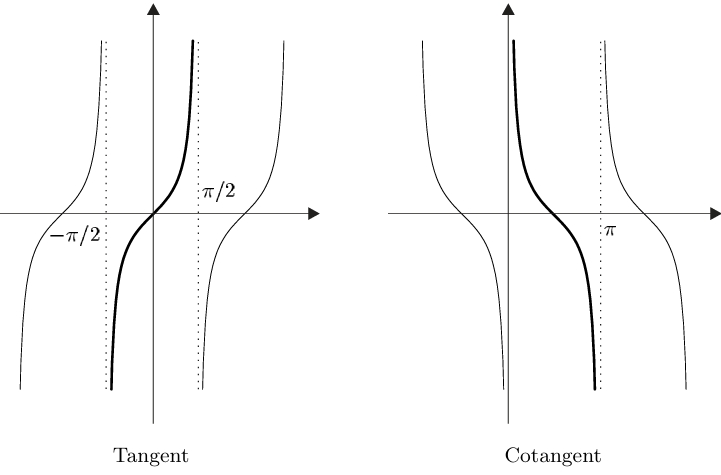
\includegraphics[height=0.4\textheight]{tang.png}
        \end{figure}
    To calculate the derivatives of the inverse trigonometric functions we use Theorem 2.8(iii). For the arcsine function this gives
    $$
    \arcsin ^{\prime} x=\frac{1}{\sin ^{\prime} y}=\frac{1}{\cos y}=\frac{1}{\sqrt{1-\sin ^2 y}}=\frac{1}{\sqrt{1-x^2}}, \quad x \in(-1,1),
    $$
    where we have set $y:=\arcsin x$ and used $x=\sin y$. Similarly, for the arctangent function,
    $$
    \arctan ^{\prime} x=\frac{1}{\tan ^{\prime} y}=\frac{1}{1+\tan ^2 y}=\frac{1}{1+x^2}, \quad x \in \mathbb{R},
    $$ 
    where $y \in(-\pi / 2, \pi / 2)$ is determined by $x=\tan y$.
    
    The derivatives of the arccosine and arccotangent functions can be calculated the same way and, summarizing, we have
    $$
    \begin{aligned}
    & \arcsin ^{\prime} x=\frac{1}{\sqrt{1-x^2}}, \quad \arccos ^{\prime} x=\frac{-1}{\sqrt{1-x^2}}, \quad x \in(-1,1), \\
    & \arctan ^{\prime} x=\frac{1}{1+x^2}, \quad \operatorname{arccot}^{\prime} x=\frac{-1}{1+x^2}, \quad x \in \mathbb{R} .
    \end{aligned}
    $$
\end{defn}
Setting: $D$ convex perfect subset of $\bb{K}$, $E$ be a Banach space, $f:D\rightarrow E$ be a function.
\begin{theo}
    For each $f \in C^n(D, E)$ and $a \in D$, there is a function $R_n(f, a) \in C(D, E)$ such that
    $$
    f(x)=\sum_{k=0}^n \frac{f^{(k)}(a)}{k!}(x-a)^k+R_n(f, a)(x), \quad x \in D
    $$  
    The remainder function $R_n(f, a)$ satisfies
    
    $$
    \left\|R_n(f, a)(x)\right\| \leq \frac{1}{(n-1)!} \sup _{0<t<1}\left\|f^{(n)}(a+t(x-a))-f^{(n)}(a)\right\||x-a|^n
    $$
    for all $x \in D$.
\end{theo}
\begin{defn}
    For $n \in \mathbb{N}, f \in C^n(D, E)$ and $a \in D$,
    $$
    \mathcal{T}_n(f, a):=\sum_{k=0}^n \frac{f^{(k)}(a)}{k!}(X-a)^k
    $$
    is a polynomial of degree $\leq n$ with coefficients in $E$, the $n^{\text {th }}$ Taylor polynomial of $f$ at $a$, and
    $$
    R_n(f, a):=f-\mathcal{T}_n(f, a)
    $$
    is the $n^{\text {th }}$ remainder function of $f$ at $a$. 
    
    Now let $E:=\mathbb{K}$ and $f \in C^{\infty}(D):=C^{\infty}(D, \mathbb{K})$. Then the formal expression
    $$
    \mathcal{T}(f, a):=\sum_k \frac{f^{(k)}(a)}{k!}(X-a)^k
    $$
    is called the Taylor series of $f$ at $a$, and by the radius of convergence of $\mathcal{T}(f, a)$ we mean the radius of convergence of the power series
    $$
    \sum_{k=0}^{\infty} \frac{f^{(k)}(a)}{k!} X^k
    $$
\end{defn}
\begin{exam}[a characterization of the exponential function]
    Suppose that $a, b \in \mathbb{C}$, the function $f: \mathbb{C} \rightarrow \mathbb{C}$ is differentiable, and
$$
f^{\prime}(z)=b f(z), \quad z \in \mathbb{C}, \quad f(0)=a
$$
Then $f(z)=a e^{b z}$ for all $z \in \mathbb{C}$.
\end{exam}
\begin{prooff}
    Notice that $f \in C^{\infty}(\mathbb{C})$ and $f^{(k)}=b^k f$ for all $k \in \mathbb{N}$. If, in addition, $f(0)=a$, then
    $$
    \sum_k \frac{f^{(k)}(0)}{k!} X^k=f(0) \sum_k \frac{b^k}{k!} X^k=a \sum_k \frac{b^k}{k!} X^k .
    $$
    Since this power series has infinite radius of convergence, we have
    $$
    \mathcal{T}(f, 0)(z)=a e^{b z}, \quad z \in \mathbb{C}
    $$
    To complete the proof, we need to prove that this Taylor series equals $f$ on $\mathbb{C}$. Notice that 
    $$
    \begin{aligned}
    \left|R_n(f, 0)(z)\right| & \leq \sup _{0<t<1}\left|f^{(n)}(t z)-f^{(n)}(0)\right| \frac{|z|^n}{(n-1)!}=\frac{|b|^n|z|^n}{(n-1)!} \sup _{0<t<1}|f(t z)-a| \\
    & \leq M|b z| \frac{|b z|^{n-1}}{(n-1)!}
    \end{aligned}
    $$
    where $M>0$ has been chosen so that $|f(w)-a| \leq M$ for all $w \in \overline{\mathbb{B}}(0,|z|)$. 
\end{prooff}



Setting: $\bb{K}=\bb{R}$ and $E=\bb{R}$. 
\begin{theo}[Schlömilch remainder formula]
    Let $I$ be a perfect interval, $a \in I$, $p>0$ and $n \in \mathbb{N}$. Suppose that $f \in C^n(I, \mathbb{R})$ and $f^{(n+1)}$ exists on $I^{\circ}$. 
    Then, for each $x \in I \backslash\{a\}$, there is some $\xi:=\xi(x) \in(\min\bbrace{x,a}, \max\bbrace{x,a})$ such that
    $$
    R_n(f, a)(x)=\frac{f^{(n+1)}(\xi)}{p n!}\left(\frac{x-\xi}{x-a}\right)^{n-p+1}(x-a)^{n+1} .
    $$

    In particular, take $p=n+1$ and $p=1$ respectively, we obtain
    $$
    R_n(f, a)(x)=\frac{f^{(n+1)}(\xi)}{(n+1)!}(x-a)^{n+1}\text{ (Lagrange)}
    $$
    and
    $$
    R_n(f, a)(x)=\frac{f^{(n+1)}(\xi)}{n!}\left(\frac{x-\xi}{x-a}\right)^n(x-a)^{n+1} \quad \text { (Cauchy) }
    $$
    
\end{theo}
\begin{exam}
Taylor series expansion for the general power function: 
$$
(1+x)^s=\sum_{k=0}^{\infty}\binom{s}{k} x^k, \quad x \in(-1,1)
$$
\end{exam}
\begin{prooff}
    Step 1: Notice that we only need to check the case when $s<0$.

    Step 2: Show that $$\binom{s}{n}=\prod_{k=1}^n(1-(s+1)/n)=\mathcal{O}(n)$$.

    Step 3: Show that, for each $x>-1$, there are some $\tau \in(0,1)$ and $\tau\p\in(0,1)$ 
    such that
    $$
    (1+x)^s=\sum_{k=0}^n\binom{s}{k} x^k+\binom{s}{n+1} \frac{x^{n+1}}{(1+\tau x)^{n+1-s}} \text{ (Lagrange)}
    $$
    and 
    $$
    (1+x)^s=\sum_{k=0}^n\binom{s}{k} x^k+\binom{s}{n+1}(n+1)(1+\tau\p x)^{s-1}x(\frac{x-\tau\p x}{1+\tau\p x})^n  \text{ (Cauchy)}
    $$

    Step 4: For $-1<x<0$,
    $$
    \frac{x-\tau\p x}{1+\tau\p x}=1-\frac{x+1}{1+\tau\p x}<-x<1
    $$
\end{prooff}
\subsection{Sequences of Functions}
Setting: $X$ is a set and $E$ be a Banach space over $\bb{K}$. 
\begin{defn}
    An $E$-valued sequence of functions on $X$ is simply a sequence $\left(f_n\right)$ in $E^X$. If the choice of $X$ and $E$ is clear from the context (or irrelevant) we say simply that $\left(f_n\right)$ is a sequence of functions.

    The sequence of functions $\left(f_n\right)$ converges pointwise to $f \in E^X$ if, for each $x \in X$, the sequence $\left(f_n(x)\right)$ converges to $f(x)$ in $E$. 
\end{defn}
\begin{defn}
    A sequence of functions $\left(f_n\right)$ converges uniformly to $f$ if, for each $\varepsilon>0$, there is some $N=N(\varepsilon) \in \mathbb{N}$ such that
    $$
    \left|f_n(x)-f(x)\right|<\varepsilon, \quad n \geq N, \quad x \in X .
    $$
\end{defn}
\begin{defn} 
    Define $B(X,E)$ be the space of bounded functions. There's a natural norm
    $$
                 f\mapsto \sup_{x\in X} |f(x)|
    $$
    on $B(X,E)$ and we denote it by $||\cdot||_{\infty}$. It's easy to check $(B(X,E),||\cdot||_{\infty})$ forms a Banach space. 

    If $f_n$ and $f$ are in $B(X, E)$, then $\left(f_n\right)$ converges uniformly to $f$ if and only if $\left(f_n\right)$ converges to $f$ in $B(X, E)$.

\end{defn}
    \begin{prop}
    The following are equivalent:
\begin{enu} 
    \item The sequence of functions $\left(f_n\right)$ converges uniformly.
    \item For each $\varepsilon>0$, there is some $N:=N(\varepsilon) \in \mathbb{N}$ such that
    $$
    \left\|f_n-f_m\right\|_{\infty}<\varepsilon, \quad n, m \geq N .
    $$
\end{enu}   
\end{prop}
\begin{defn}
    Let $\left(f_k\right)$ be an $E$-valued sequence of functions on $X$, that is, a sequence in $E^X$. Then
    $$
    s_n:=\sum_{k=0}^n f_k \in E^X, \quad n \in \mathbb{N}
    $$
    and so we have a well defined sequence $\left(s_n\right)$ in $E^X$. 
    
    The series $\sum f_k$ is called   
    $$
    \begin{aligned}
    \text { pointwise convergent } & : \Leftrightarrow \sum f_k(x) \text { converges in } E \text { for each } x \in X, \\
    \text { absolutely convergent } & : \Leftrightarrow \sum\left|f_k(x)\right|<\infty \text { for each } x \in X, \\
    \text { uniformly convergent } & : \Leftrightarrow\left(s_n\right) \text { converges uniformly, } \\
    \text { norm convergent } & : \Leftrightarrow \sum\left\|f_k\right\|_{\infty}<\infty .
    \end{aligned}
    $$
\end{defn}
\begin{rema}
    If $f_k$ is norm convergent, then by Proposition\,\ref{complete iff absolutely convergent}, $f_k\mapsto f$ for some $f\in B(X,E)$. 
    Hence, $f_k$ is uniformly convergent and absolutely convergent.
\end{rema}
\begin{theo}[Weierstrass majorant criterion]
    Suppose that $f_k \in B(X, E)$ for all $k \in \mathbb{N}$. If there is a convergent series $\sum \alpha_k$ in $\mathbb{R}$ such that $\left\|f_k\right\|_{\infty} \leq \alpha_k$ for almost all $k \in \mathbb{N}$, then $\sum f_k$ is norm convergent. In particular, $\sum f_k$ converges absolutely and uniformly.
\end{theo}
\begin{theo}
    Let $\sum a_k Y^k$ be a power series with positive radius of convergence $\rho$ and $0<r<\rho$. Then the series $\sum a_k Y^k$ is norm convergent on $r \overline{\mathbb{B}}_{\mathbb{K}}$. In particular, it converges absolutely and uniformly.
\end{theo}
Setting: $X$ metric space, $E$ be a Banach space. 
\begin{defn}
    A sequence of functions $\left(f_n\right)$ is called locally uniformly convergent if each $x \in X$ has a neighborhood $U$ such that $\left(f_n \mid U\right)$ converges uniformly. A series of functions $\sum f_n$ is called locally uniformly convergent if the sequence of partial sums $\left(s_n\right)$ converges locally uniformly.
\end{defn}
\begin{theo}
    If a sequence of continuous functions $\left(f_n\right)$ converges locally uniformly to $f$, then $f$ is also continuous. In other words, locally uniform limits of continuous functions are continuous.
\end{theo}
\begin{theo}[differentiability of the limits of sequences of functions]
    Let $X$ be an open subset of $\mathbb{K}$ and $f_n \in C^1(X, E)$ for all $n \in \mathbb{N}$. Suppose that there are $f, g \in E^X$ such that
\begin{enu}     
    \item $\left(f_n\right)$ converges pointwise to $f$, and
    \item $\left(f_n^{\prime}\right)$ converges locally uniformly to $g$.
\end{enu}
    Then $f$ is in $C^1(X, E)$, and $f^{\prime}=g$. In addition, $\left(f_n\right)$ converges locally uniformly to $f$.
\end{theo}
% \begin{prooff}
%     Step 1: $f_n\p\in C(X,E)$ converges locally uniformly to $g$, then $g\in C(X,E)$。 
    
%     Step 2: Let $a \in X$. Then there is some $r>0$ such that $\left(f_n^{\prime}\right)$ converges uniformly to $g$ on $B_r:=\mathbb{B}_{\mathbb{K}}(a, r) \subset X$. Thus, for each $x \in B_r$, we can apply the mean value theorem to the function
%     $$
%     [0,1] \rightarrow E, \quad t \mapsto f_n(a+t(x-a))-t f_n^{\prime}(a)(x-a)
%     $$
%     to get
%     $$
%     \left|f_n(x)-f_n(a)-f_n^{\prime}(a)(x-a)\right| \leq \sup _{0<t<1}\left|f_n^{\prime}(a+t(x-a))-f_n^{\prime}(a)\right||x-a| .
%     $$
%     Taking the limit $n \rightarrow \infty$ we get
%     $$
%     |f(x)-f(a)-g(a)(x-a)| \leq \sup _{0<t<1}|g(a+t(x-a))-g(a)||x-a|
%     $$
%     for each $x \in B_r$. Step 1 shows that $g$ is in $C(X, E)$, so 
%     $$
%     f(x)-f(a)-g(a)(x-a)=o(|x-a|)(x \rightarrow a) .
%     $$
%     Hence $f$ is differentiable at $a$ and $f^{\prime}(a)=g(a)$. Since this holds for all $a \in X$, we have shown that $f \in C^1(X, E)$.

%     Step 3: Now we show that $f$ is locally uniquely continous: for $x\in B_r$, 
%     \begin{equation*}
%         \begin{aligned}
%             \left|f_n(x)-f(x)\right| & \leq\left|f_n(x)-f(x)-\left(f_n(a)-f(a)\right)\right|+\left|f_n(a)-f(a)\right| \\
%             & \leq r \sup _{0<t<1}\left|f_n^{\prime}(a+t(x-a))-f^{\prime}(a+t(x-a))\right|+\left|f_n(a)-f(a)\right| \\
%         \end{aligned}
%     \end{equation*}

% \end{prooff} 
\begin{coro}
    Suppose that $X \subseteq \mathbb{K}$ is open, and $\left(f_n\right)$ is a sequence in $C^1(X, E)$ for which $\sum_n f_n$ converges pointwise and $\sum f_n^{\prime}$ converges locally uniformly. Then the $\operatorname{sum} \sum_{n=0}^{\infty} f_n$ is in $C^1(X, E)$ and
    $$
    \left(\sum_{n=0}^{\infty} f_n\right)^{\prime}=\sum_{n=0}^{\infty} f_n^{\prime}
    $$
    \label{corollary: sum of partial fn}
\end{coro}

Setting: Let $a=\sum_k a_k X^k \in \mathbb{K} \llbracket X \rrbracket$ be a power series with radius of convergence $\rho=\rho_a>0$, and $\underline{a}$ the function on $\rho \mathbb{B}_{\mathbb{K}}$ represented by $a$. When no misunderstanding is possible, we write $\mathbb{B}$ for $\mathbb{B}_{\mathbb{K}}$.
\begin{theo}
    Let $a=\sum_k a_k X^k$ be a power series. Then $\underline{a}$ is continuously differentiable on $\rho \mathbb{B}$. The 'termwise differentiated' series $\sum_{k \geq 1} k a_k X^{k-1}$ has radius of convergence $\rho$ and
    $$
    \underline{a}^{\prime}(x)=\left(\sum_{k=0}^{\infty} a_k x^k\right)^{\prime}=\sum_{k=1}^{\infty} k a_k x^{k-1}, \quad x \in \rho \mathbb{B} .
    $$
\end{theo}
\begin{coro}
    If $a=\sum a_k X^k$ is a power series with positive radius of convergence $\rho$, then $\underline{a} \in C^{\infty}(\rho \mathbb{B}, \mathbb{K})$ and $a_k=\underline{a}^{(k)}(0)/k!$.
\end{coro}
\begin{defn}
    Let $D$ be open in $\mathbb{K}$. A function $f: D \rightarrow \mathbb{K}$ is called analytic (on $D$ ) if, for each $x_0 \in D$, there is some $r=r\left(x_0\right)>0$ such that $\mathbb{B}\left(x_0, r\right) \subseteq D$ and a power series $\sum_k a_k X^k$ with radius of convergence $\rho \geq r$, such that
    $$
    f(x)=\sum_{k=0}^{\infty} a_k\left(x-x_0\right)^k, \quad x \in \mathbb{B}\left(x_0, r\right) .
    $$
    In this case, we say that $\sum_k a_k\left(X-x_0\right)^k$ is the power series expansion for $f$ at $x_0$. The set of all analytic functions on $D$ is denoted by $C^\omega(D, \mathbb{K})$, or by $C^\omega(D)$ if no misunderstanding is possible. Further, $f \in C^\omega(D)$ is called real (or complex) analytic if $\mathbb{K}=\mathbb{R}($ or $\mathbb{K}=\mathbb{C})$.
\end{defn}
\begin{prop}[A power series represents an analytic function on its disk of convergence]
    Suppose that $a=\sum a_k X^k$ is a power series with radius of convergence $\rho>0$. Then $\underline{a} \in C^\omega(\rho \mathbb{B}, \mathbb{K})$ and
    $$
    \underline{a}(x)=\mathcal{T}\left(\underline{a}, x_0\right)(x), \quad x_0 \in \rho \mathbb{B}, \quad x \in \mathbb{B}\left(x_0, \rho-\left|x_0\right|\right) .
    $$
\end{prop}
\begin{defn}
    A nonempty open and connected subset of a metric space is called a domain.
\end{defn}
Setting: Suppose that $D$ is open in $\mathbb{K}$, 
$E$ is a normed vector space and $f: D \rightarrow E$.
\begin{defn}
$F: D \rightarrow E$ is called an antiderivative of $f$ if $F$ is differentiable and $F^{\prime}=f$.
\end{defn}
\begin{prop}
    Let $D \subseteq \mathbb{K}$ be a domain and $f: D \rightarrow E$. If $F_1, F_2 \in E^D$ are antiderivatives of $f$, then $F_2-F_1$ is constant. That is, antiderivatives are unique up to an additive constant.
\end{prop}
\begin{coro}
    Let $E=\mathbb{K}$. If $f \in C^\omega(D, \mathbb{K})$  has an antiderivative $F$, then $F$ is also analytic.
\end{coro}
\begin{prooff}
Let $x_0 \in D$. Then there is some $r>0$ such that
$$
f(x)=\sum_{k=0}^{\infty} \frac{f^{(k)}\left(x_0\right)}{k!}\left(x-x_0\right)^k, \quad x \in \mathbb{B}\left(x_0, r\right) \subseteq D .
$$
Then, there is some $a \in \mathbb{K}$ such that
$$
F(x)=a+\sum_{k=0}^{\infty} \frac{f^{(k)}\left(x_0\right)}{(k+1)!}\left(x-x_0\right)^{k+1}, \quad x \in \mathbb{B}\left(x_0, r\right) .
$$
Them, $F$ is analytic on $\mathbb{B}\left(x_0, r\right)$. Since analyticity is a local property, the claim follows.
\end{prooff}
\begin{theo}
    Let $D$ be a domain in $\mathbb{K}$ and $f \in C^\omega(D, \mathbb{K})$. If the set of zeros of $f$ has a limit point in $D$, then $f$ is zero on $D$.
\end{theo}
\begin{exam}
    Define $\log z=\log re^{i\theta}=\log r+i\theta$ for $\theta\in (-\pi,\pi)$. Then $\log z$ is a analytic function on 
    $\bb{C}-(-\infty,0]$. 
\end{exam}
\begin{prooff}
   It's easy to show that $(\log z)\p=1/z$. 
   And notice that 
   $$
   \frac{1}{z}=\sum_{k=0}^{\infty} \frac{(-1)^k}{z_0^{k+1}}\left(z-z_0\right)^k, \quad z_0 \in \mathbb{C}^{\times}, \quad z \in \mathbb{B}_{\mathbb{C}}\left(z_0,\left|z_0\right|\right)
   $$, 
we have $1/z$ is analytic in $\bb{C}-(-\infty,0]$. By above Corollary, for some $c\in \bb{C}$, 
$$
\log z=c+\sum_{k=0}^{\infty} \frac{(-1)^k}{(k+1) z_0^{k+1}}\left(z-z_0\right)^{k+1}, \quad z, z_0 \in \mathbb{C} \backslash(-\infty, 0], \quad\left|z-z_0\right|<\left|z_0\right|
$$
In particular, for all $z \in \mathbb{B}_{\mathbb{C}}$,
$$
\log (1+z)=\sum_{k=1}^{\infty}(-1)^{k-1} z^k / k
$$


\end{prooff}
\begin{exam}
For $z\in 1+\bb{B}_\bb{C}$ and $\alpha\in \bb{C}-\bb{N}$, 
define $z^\alpha=e^{\alpha\log z}$, we have 
$$
\sum_{k=0}^{\infty}\binom{\alpha}{k} z^k=(1+z)^\alpha, \quad z \in \mathbb{B}_{\mathbb{C}}
$$
\end{exam}
\begin{prooff}
    Let $a_k:=\binom{\alpha}{k}$. Since $\alpha \notin \mathbb{N}$ we have $\lim \left|a_k / a_{k+1}\right|=\lim _k((k+1) /|\alpha-k|)=1$, the binomial series has radius of convergence 1 .
Define $f(z):=\sum_{k=0}^{\infty} a_k z^k$ for all $z \in \mathbb{B}_{\mathbb{C}}$. We have
$$
(1+z) f^{\prime}(z)-\alpha f(z)=0, \quad z \in \mathbb{B}_{\mathbb{C}},
$$
from which follows
$$
\left[(1+z)^{-\alpha} f(z)\right]^{\prime}=(1+z)^{-\alpha-1}\left[(1+z) f^{\prime}(z)-\alpha f(z)\right]=0, \quad z \in \mathbb{B}_{\mathbb{C}}
$$
Since $\mathbb{B}_{\mathbb{C}}$ is a domain, $(1+z)^{-\alpha} f(z)=c$ for some constant $c \in \mathbb{C}$. Since $f(0)=1$, we have $c=1$, and so $f(z)=(1+z)^\alpha$ for all $z \in \mathbb{B}_{\mathbb{C}}$.
\end{prooff}
\begin{exam}[The case $\alpha=1 / 2$]
    First we calculate the binomial coefficients:
    $$
    \begin{aligned}
    \binom{1 / 2}{k} & =\frac{1}{k!} \frac{1}{2}\left(\frac{1}{2}-1\right) \cdot \cdots \cdot\left(\frac{1}{2}-k+1\right) \\
    & =\frac{(-1)^{k-1}}{k!} \frac{1 \cdot 3 \cdot \cdots \cdot(2 k-3)}{2^k} \\
    & =(-1)^{k-1} \frac{1 \cdot 3 \cdot \cdots \cdot(2 k-3)}{2 \cdot 4 \cdot \cdots \cdot 2 k}
    \end{aligned}
    $$
    for all $k \geq 2$. We get the series expansion
    $$
    \sqrt{1+z}=1+\frac{z}{2}+\sum_{k=2}^{\infty}(-1)^{k-1} \frac{1 \cdot 3 \cdot \cdots \cdot(2 k-3)}{2 \cdot 4 \cdot \cdots \cdot 2 k} z^k, \quad z \in \mathbb{B}_{\mathbb{C}}
    $$   
\end{exam}
\begin{exam}[The case $\alpha=-1/2$]
    Here we have
    $$
    \binom{-1 / 2}{k}=(-1)^k \frac{1 \cdot 3 \cdot \cdots \cdot(2 k-1)}{2 \cdot 4 \cdot \cdots \cdot 2 k}, \quad k \geq 2
    $$
    We get
    $$
    \frac{1}{\sqrt{1+z}}=1-\frac{z}{2}+\sum_{k=2}^{\infty}(-1)^k \frac{1 \cdot 3 \cdot \cdots \cdot(2 k-1)}{2 \cdot 4 \cdot \cdots \cdot 2 k} z^k, \quad z \in \mathbb{B}_{\mathbb{C}} .
    $$
    If $|z|<1$ then $\left|-z^2\right|<1$ and so we can substitute $-z^2$ for $z$ to get
    $$
    \frac{1}{\sqrt{1-z^2}}=1+\frac{z^2}{2}+\sum_{k=2}^{\infty} \frac{1 \cdot 3 \cdot \cdots \cdot(2 k-1)}{2 \cdot 4 \cdot \cdots \cdot 2 k} z^{2 k}, \quad z \in \mathbb{B}_{\mathbb{C}} .
    $$  
\end{exam}
\begin{exam}
    The arcsine function is real analytic on $(-1,1)$ and
$$
\arcsin (x)=x+\sum_{k=1}^{\infty} \frac{1 \cdot 3 \cdot \cdots \cdot(2 k-1)}{2 \cdot 4 \cdot \cdots \cdot 2 k} \frac{x^{2 k+1}}{2 k+1}, \quad x \in(-1,1) .
$$
\end{exam}



\newpage
\section{Multivariable Differential Calculus}
\subsection{Differentiability}
Setting: 
$E=(E,\|\cdot\|)$ and $F=(F,\|\cdot\|)$ are Banach spaces
over the field $\mathbb{K}$, $X$ open subset of $E$ and 
$\mathcal{L}(E, F)$, the space of all bounded linear maps from $E$ to $F$.
\begin{defn}
    A function $f: X \rightarrow F$ is differentiable at $x_0 \in X$ if there is an $A_{x_0} \in \mathcal{L}(E, F)$ such that
    $$
    \lim _{x \rightarrow x_0} \frac{f(x)-f\left(x_0\right)-A_{x_0}\left(x-x_0\right)}{\left\|x-x_0\right\|}=0 .
    $$
\end{defn}
\begin{defn}
    Suppose $f: X \rightarrow F$ is differentiable at $x_0 \in X$. Then we denote by $\partial f\left(x_0\right)$ the linear operator $A_{x_0} \in \mathcal{L}(E, F)$ uniquely determined. 
    This is called the derivative of $f$ at $x_0$ and will also be written
    $$
    D f\left(x_0\right) \text { or } f^{\prime}\left(x_0\right) \text {. }
    $$
    Therefore $\partial f\left(x_0\right) \in \mathcal{L}(E, F)$, and
    $$
    \lim _{x \rightarrow x_0} \frac{f(x)-f\left(x_0\right)-\partial f\left(x_0\right)\left(x-x_0\right)}{\left\|x-x_0\right\|}=0 .
    $$
    If $f: X \rightarrow F$ is differentiable at every point $x \in X$, we say $f$ is differentiable and call the map
    $$
    \partial f: X \rightarrow \mathcal{L}(E, F), \quad x \mapsto \partial f(x)
    $$
    the derivative of $f$.
    Since $\mathcal{L}(E, F)$ is a Banach space, we can meaningfully speak of the continuity of the derivative. If $\partial f$ is continuous, that is, $\partial f \in C(X, \mathcal{L}(E, F))$, we call $f$ continuously differentiable. We set
    $$
    C^1(X, F):=\{f: X \rightarrow F ; f \text { is continuously differentiable }\} .
    $$
\end{defn}
\begin{defn}[Directional derivatives]
    Suppose $f: X \rightarrow F, x_0 \in X$ and $v \in E \backslash\{0\}$. Because $X$ is open, there is an $\varepsilon>0$ such that $x_0+t v \in X$ for $|t|<\varepsilon$. Therefore the function
    $$
    (-\varepsilon, \varepsilon) \rightarrow F, \quad t \mapsto f\left(x_0+t v\right)
    $$
    is well defined. When this function is differentiable at the point 0 , we call its derivative the directional derivative of $f$ at the point $x_0$ in the direction $v$ and denote it by $D_v f\left(x_0\right)$. Thus
    $$
    D_v f\left(x_0\right)=\lim _{t \rightarrow 0} \frac{f\left(x_0+t v\right)-f\left(x_0\right)}{t}
    $$
\end{defn}
\begin{prop}
    Suppose $f: X \rightarrow F$ is differentiable at $x_0 \in X$. Then $D_v f\left(x_0\right)$ exists for every $v \in E \backslash\{0\}$, and $D_v f\left(x_0\right)=\partial f\left(x_0\right) v$.
\end{prop}
\begin{exam}
    We consider a function $f: \mathbb{R}^2 \rightarrow \mathbb{R}$ defined by
    $$
    f(x, y):=\left\{\begin{array}{cl}
    \dfrac{x^2 y}{x^2+y^2}, & (x, y) \neq(0,0) \\
    0, & (x, y)=(0,0)
    \end{array}\right.
    $$
    For every $v=(\xi, \eta) \in \mathbb{R}^2 \backslash\{(0,0)\}$, we have
    $$
    f(t v)=\frac{t^3 \xi^2 \eta}{t^2\left(\xi^2+\eta^2\right)}=t f(v)
    $$
    Thus
    $$
    D_v f(0)=\lim _{t \rightarrow 0} f(t v) / t=f(v)
    $$
    If $f$ were differentiable at 0, $\partial f(0) v=D_v f(0)=f(v)$ for every $v \in \mathbb{R}^2 \backslash\{(0,0)\}$. A contridiction! 
\end{exam}
\begin{defn}
    Suppose $X$ is open in $\mathbb{R}^n$ and $f=\left(f^1, \ldots, f^m\right): X \rightarrow \mathbb{R}^m$ is partially differentiable at $x_0$. We then call
    $$
    \left[\partial_k f^j\left(x_0\right)\right]=\left[\begin{array}{ccc}
    \partial_1 f^1\left(x_0\right) & \cdots & \partial_n f^1\left(x_0\right) \\
    \vdots & & \vdots \\
    \partial_1 f^m\left(x_0\right) & \cdots & \partial_n f^m\left(x_0\right)
    \end{array}\right]
    $$
    the Jacobi matrix of $f$ at $x_0$.
\end{defn}
\begin{prop}
    Suppose $X$ is open in $\mathbb{R}^n$ and $F$ is a Banach space. Then $f: X \rightarrow F$ is continuously differentiable if and only if $f$ has continuous partial derivatives.
\end{prop}
\begin{coro}
    Let $X$ be open in $\mathbb{R}^n$. Then $f: X \rightarrow \mathbb{R}^m$ is continuously differentiable if and only if every coordinate function $f^j: X \rightarrow \mathbb{R}$ has continuous partial derivatives, and then
    $$
    [\partial f(x)]=\left[\partial_k f^j(x)\right] \in \mathbb{R}^{m \times n}
    $$
\end{coro}
\begin{theo}[Cauchy-Riemann Equation]
    Suppose $X$ is open at $\mathbb{C}$. For $f: X \rightarrow \mathbb{C}$, we set $u:=\operatorname{Re} f$ and $v:=\operatorname{Im} f$.

    The function $f$ is complex differentiable at $z_0=x_0+i y_0$ if and only if $F:=(u, v)$ is 
    differentiable(as a function$f:X\subset \bb{R}^2\rightarrow \bb{R}^2$) at $\left(x_0, y_0\right)$ and satisfies the Cauchy-Riemann equations 
    $$
    u_x=v_y, \quad u_y=-v_x
    $$
    at $\left(x_0, y_0\right)$. In that case,
    $$
    f^{\prime}\left(z_0\right)=u_x\left(x_0, y_0\right)+i v_x\left(x_0, y_0\right)
    $$
    
\end{theo}
\begin{prooff}
    Suppose $f$ is complex differentiable at $z_0$. We set
$$
A:=\left[\begin{array}{cc}
\alpha & -\beta \\
\beta & \alpha
\end{array}\right]
$$
where $\alpha:=\operatorname{Re} f^{\prime}\left(z_0\right)$ and $\beta:=\operatorname{Im} f^{\prime}\left(z_0\right)$. Then for $h=\xi+i \eta \longleftrightarrow(\xi, \eta)$, we have
$$
\begin{aligned}
\lim _{\left(\xi, \eta\right) \rightarrow(0,0)} \frac{\left|F\left(x_0+\xi, y_0+\eta\right)-F\left(x_0, y_0\right)-A(\xi, \eta)\right|}{|(\xi, \eta)|} \\
\quad=\lim _{h \rightarrow 0}\left|\frac{f\left(z_0+h\right)-f\left(z_0\right)-f^{\prime}\left(z_0\right) h}{h}\right|=0
\end{aligned}
$$
Therefore $F$ is totally differentiable
$$
\left[\partial F\left(x_0, y_0\right)\right]=\left[\begin{array}{ll}
\partial_1 u\left(x_0, y_0\right) & \partial_2 u\left(x_0, y_0\right) \\
\partial_1 v\left(x_0, y_0\right) & \partial_2 v\left(x_0, y_0\right)
\end{array}\right]=\left[\begin{array}{cc}
\alpha & -\beta \\
\beta & \alpha
\end{array}\right]
$$

\end{prooff}
\begin{theo}[chain rule]
    Suppose $Y$ is open in $F$ and $G$ is a Banach space. Also suppose $f: X \rightarrow F$ is differentiable at $x_0$ and $g: Y \rightarrow G$ is differentiable at $y_0:=f\left(x_0\right)$ and that $f(X) \subset Y$. Then $g \circ f: X \rightarrow G$ is differentiable at $x_0$, and the derivative is given by
    $$
    \partial(g \circ f)\left(x_0\right)=\partial g\left(f\left(x_0\right)\right) \partial f\left(x_0\right) .
    $$
\end{theo}
\begin{theo}[mean value theorem in integral form]
    In what follows, we use the notation $\llbracket x, y \rrbracket$ for the straight path $\{x+t(y-x) ; t \in[0,1]\}$ 
    between the points $x, y \in E$.
    Let $f \in C^1(X, F)$. Then we have
    $$
    f(y)-f(x)=\int_0^1 \partial f(x+t(y-x))(y-x) d t
    $$
    for $x, y \in X$ such that $\llbracket x, y \rrbracket \subset X$.
\end{theo}
\begin{prooff}
    By Hahn-Banach Theorem,  fundamental theorem of calculus and Proposition\,\ref{Proposition: Intergration commutes with linear transform}. 
\end{prooff}
\begin{coro}
    $X$ be a connect open subset of $X$, $f\in C^1(X,F)$, then if $\partial f=0$, $f$ is a constant. 
\end{coro}










\subsection{Continuous Multilinear Map}
Setting: 
In the following, $E_1, \ldots, E_m$ for $m \geq 2, E$, and $F$ are Banach spaces over the field $\mathbb{K}$. 
\begin{defn} 
A map $\varphi: E_1 \times \cdots \times E_m \rightarrow F$ is multilinear or, equivalently, $m$-linear if for every $k \in\{1, \ldots, m\}$ and every choice of $x_j \in E_j$ for $j=1, \ldots, m$ with $j \neq k$, the map
$$
\varphi\left(x_1, \ldots, x_{k-1}, \cdot, x_{k+1}, \ldots, x_m\right): E_k \rightarrow F
$$
is linear.
\end{defn}
\begin{prop}
    For the m-linear map $\varphi: E_1 \times \cdots \times E_m \rightarrow F$, these statements are equivalent:
\begin{enu} 
    \item $\varphi$ is continuous.
    \item $\varphi$ is continuous at 0 .
    \item $\varphi$ is bounded on bounded sets.
    \item There is an $\alpha \geq 0$ such that
    $$
    \left\|\varphi\left(x_1, \ldots, x_m\right)\right\| \leq \alpha\left\|x_1\right\| \cdots \cdots\left\|x_m\right\| \quad \text { for } x_j \in E_j, \quad 1 \leq j \leq m
    $$
\end{enu}
\end{prop}
\begin{theo}
    Define
    $$
    \|\varphi\|:=\inf \left\{\alpha \geq 0 ;\left\|\varphi\left(x_1, \ldots, x_m\right)\right\| \leq \alpha\left\|x_1\right\| \cdots \cdots x_m \|, x_j \in E_j\right\}
    $$
    for $\varphi \in \mathcal{L}\left(E_1, \ldots, E_m ; F\right)$.
    
    Then
    $$
    \|\varphi\|=\sup \left\{\left\|\varphi\left(x_1, \ldots, x_m\right)\right\| ;\left\|x_j\right\| \leq 1,1 \leq j \leq m\right\}
    $$
    and
    $$
    \mathcal{L}\left(E_1, \ldots, E_m ; F\right):=\left(\mathcal{L}\left(E_1, \ldots, E_m ; F\right),\|\cdot\|\right)
    $$
    is a Banach space.
\end{theo}
\begin{theo}
    The spaces $\mathcal{L}\left(E_1, \ldots, E_m ; F\right)$ and $\mathcal{L}\left(E_1, \mathcal{L}\left(E_2, \ldots, \mathcal{L}\left(E_m, F\right) \ldots\right)\right)$ are isometrically isomorphic.
\end{theo}
\begin{prooff} 
    We verify the statement for $m=2$. The general case obtains via a simple induction argument.
     
    Firstly, for $T \in \mathcal{L}\left(E_1, \mathcal{L}\left(E_2, F\right)\right)$ we set
    $$
    \varphi_T\left(x_1, x_2\right):=\left(T x_1\right) x_2 \quad \text { for }\left(x_1, x_2\right) \in E_1 \times E_2
    $$
    Then $\varphi_T: E_1 \times E_2 \rightarrow F$ is bilinear, and
    $$
    \left\|\varphi_T\left(x_1, x_2\right)\right\| \leq\|T\|\left\|x_1\right\|\left\|x_2\right\| \quad \text { for }\left(x_1, x_2\right) \in E_1 \times E_2 .
    $$
    Therefore $\varphi_T$ belongs to $\mathcal{L}\left(E_1, E_2 ; F\right)$, and $\left\|\varphi_T\right\| \leq\|T\|$.
    
    Secondly, suppose $\varphi \in \mathcal{L}\left(E_1, E_2 ; F\right)$. Then we set
    $$
    T_{\varphi}\left(x_1\right) x_2:=\varphi\left(x_1, x_2\right) \quad \text { for }\left(x_1, x_2\right) \in E_1 \times E_2
    $$
    Because
    $$
    \left\|T_{\varphi}\left(x_1\right) x_2\right\|=\left\|\varphi\left(x_1, x_2\right)\right\| \leq\|\varphi\|\left\|x_1\right\|\left\|x_2\right\| \quad \text { for }\left(x_1, x_2\right) \in E_1 \times E_2
    $$
    we get
    $$
    T_{\varphi}\left(x_1\right) \in \mathcal{L}\left(E_2, F\right) \quad \text { for }\left\|T_{\varphi}\left(x_1\right)\right\| \leq\|\varphi\|\left\|x_1\right\|
    $$
    for every $x_1 \in E_1$. Therefore
    $$
    T_{\varphi}:=\left[x_1 \mapsto T_\psi\left(x_1\right)\right] \in \mathcal{L}\left(E_1, \mathcal{L}\left(E_2, F\right)\right) \text { and }\left\|T_\psi\right\| \leq\|\varphi\|
    $$
    
    Altogether, we have proved that the maps
    $$
    T \mapsto \varphi_{\mathrm{T}}: \mathcal{L}\left(E_1, \mathcal{L}\left(E_2, F\right)\right) \rightarrow \mathcal{L}\left(E_1, E_2 ; F\right)
    $$
    and
    $$
    \varphi \mapsto T_\psi: \mathcal{L}\left(E_1, E_2 ; F\right) \rightarrow \mathcal{L}\left(E_1, \mathcal{L}\left(E_2, F\right)\right)
    $$
    are linear, bijective, isometry.
\end{prooff}
\begin{prop}
    Suppose $m \geq 2$ and $\varphi: E^m \rightarrow F$ is $m$-linear. We say $\varphi$ is symmetric if
    $$
    \varphi\left(x_{\sigma(1)}, \ldots, x_{\sigma(m)}\right)=\varphi\left(x_1, \ldots, x_m\right)
    $$
    for every $\left(x_1, \ldots, x_m\right)$ and every permutation $\sigma$ of $\{1, \ldots, m\}$. We set
    $$
    \mathcal{L}_{\mathrm{sym}}^m(E, F):=\left\{\varphi \in \mathcal{L}^m(E, F) ; \varphi \text { is symmetric }\right\}
    $$
    
    $\mathcal{L}_{\text {sym }}^m(E, F)$ is a 
    closed vector subspace of $\mathcal{L}^m(E, F)$ and is therefore itself a Banach space.
\end{prop}
\begin{prop}
$\mathcal{L}\left(E_1, \ldots, E_m ; F\right)$ is a vector subspace of $C^1\left(E_1 \times \cdots \times E_m, F\right)$. And, for $\varphi \in \mathcal{L}\left(E_1, \ldots, E_m ; F\right)$ and $\left(x_1, \ldots, x_m\right) \in E_1 \times \cdots \times E_m$, we have
$$
\partial \varphi\left(x_1, \ldots, x_m\right)\left(h_1, \ldots, h_m\right)=\sum_{j=1}^m \varphi\left(x_1, \ldots, x_{j-1}, h_j, x_{j+1}, \ldots, x_m\right)
$$
for $\left(h_1, \ldots, h_m\right) \in E_1 \times \cdots \times E_m$.
\label{proposition: mul-linear map is C1}
\end{prop} 
\begin{prooff}
 
\end{prooff}
% Setting: 
% $E=(E,\|\cdot\|)$ and $F=(F,\|\cdot\|)$ are Banach spaces
% over the field $\mathbb{K}$, $X$ open subset of $E$ and 
% $\mathcal{L}(E, F)$, the space of all bounded linear maps from $E$ to $F$.
\begin{defn}
    Suppose $f: X \rightarrow F$ and $x_0 \in X$. We then set $\partial^0 f:=f$. Therefore $\partial^0 f\left(x_0\right)$ belongs to $F=\mathcal{L}^0(E, F)$. Suppose now that $m \in \mathbb{N}^{\times}$and $\partial^{m-1} f: X \rightarrow$ $\mathcal{L}^{m-1}(E, F)$ is already defined. If
    $$
    \partial^m f\left(x_0\right):=\partial\left(\partial^{m-1} f\right)\left(x_0\right) \in \mathcal{L}\left(E, \mathcal{L}^{m-1}(E, F)\right)=\mathcal{L}^m(E, F)
    $$
    exists, we call $\partial^m f\left(x_0\right)$ the 
    $m$-th derivative of $f$ at $x_0$, we call
    $$
    \partial^m f: X \rightarrow \mathcal{L}^m(E, F)
    $$
    the $m$-th derivative of $f$.
    We set
    $$
    C^m(X, F):=\{f: X \rightarrow F ; f \text { is } m \text {-times continuously differentiable }\}
    $$
    and
    $$
    C^{\infty}(X, F):=\bigcap_{m \in \mathbb{N}} C^m(X, F)
    $$
\end{defn}
\begin{prop}
    For $f \in C^m(X, F)$ such that $m \geq 2$, we have $\partial^m f(x) \in \mathcal{L}_{\text {sym }}^m(E, F) \quad$ for $x \in X$.
\end{prop}
\begin{prop}[chain rule]
    Suppose $Y$ is open in $F$ and $G$ is a Banach space. Also suppose $m \in \mathbb{N}^{\times}$and $f \in C^m(X, F)$ with $f(X) \subset Y$ and $g \in C^m(Y, G)$. Then we have $g \circ f \in C^m(X, G)$.
\end{prop}
\begin{prop}
    We consider first the case $E=\mathbb{R}^n$ with $n \geq 2$.
    For $q \in \mathbb{N}^{\times}$and indices $j_1, \ldots, j_q \in\{1, \ldots, n\}$, we call
    $$
    \frac{\partial^q f(x)}{\partial x^{j_1} \partial x^{j_2} \cdots \partial x^{j_q}}:=\partial_{j_1} \partial_{j_2} \cdots \partial_{j_q} f(x) \quad \text { for } x \in X
    $$
    
    Suppose $X$ is open in $\mathbb{R}^n, f: X \rightarrow F$, and $m \in \mathbb{N}^{\times}$. Then the following statements hold:
    \begin{enu}
    \item $f$ belongs to $C^m(X, F)$ if and only if $f$ is $m$-times continuously partially differentiable.
    \item For $f \in C^m(X, F)$, we have
    \end{enu}
    $$
    \frac{\partial^q f}{\partial x^{j_1} \cdots \partial x^{j_q}}=\frac{\partial^q f}{\partial x^{j_{\sigma(1)}} \cdots \partial x^{j_{\sigma(q)}}} \quad \text { for } 1 \leq q \leq m
    $$
    for every permutation $\sigma \in \mathrm{S}_q$, that is, the partial derivatives are independent of the order of differentiation. 
\end{prop}
% \begin{prooff}
%     (1): If $m=2$ and $f\in C^2(X,F)$, we have 
%     \begin{equation*}
%         \lim_{h\to 0} \frac{\partial f(x+h)-\partial f(x)-\partial^2 f(x)(h)}{h}=0.
%     \end{equation*}
%     Since
%     $\partial f(x)(h_1):X\rightarrow F\in C(X,F)$, 
%     we have 
%     \begin{equation*}
%         \lim_{h\to 0} \frac{\partial f(x+h)(h_1)-\partial f(x)(h_1)-
%         \partial^2 f(x)(h,h_1)}{h}=0.
%     \end{equation*}
%     Since, $\partial^2 f(x)(h,h_1)=\partial^2 f(x)(h_1,h)$, we have 
%     $\partial(\partial f(x)(h_1))=\partial^2 f(x)(h_1,\cdot)$.





% \end{prooff}
\begin{theo}[Taylor's theorem]
    Define
    $$
    \partial^k f(x)[h]^k:=\left\{\begin{array}{lr}
    \partial^k f(x)[\underbrace{h, \ldots, h}_{k \text {-times }}], & 1 \leq k \leq q \\
    f(x), & k=0
    \end{array}\right.
    $$
    
    For $x \in X, h \in E$, and $f \in C^q(X, F)$.
    Suppose $X$ is open in $E, q \in \mathbb{N}^{\times}$, and $f$ belongs to $C^q(X, F)$. Then
    $$
    f(x+h)=\sum_{k=0}^q \frac{1}{k!} \partial^k f(x)[h]^k+R_q(f, x ; h)
    $$
    for $x \in X$ and $h \in E$ such that $\llbracket x, x+h \rrbracket \subset X$. Here
    $$
    R_q(f, x ; h):=\int_0^1 \frac{(1-t)^{q-1}}{(q-1)!}\left[\partial^q f(x+t h)-\partial^q f(x)\right][h]^q d t \in F
    $$
    is the $q$-th order remainder of $f$ at the point $x$.
\end{theo}




\subsection{Inverse maps and Implicit functions}
Setting: $E$ and $F$ are Banach spaces over the field $\mathbb{K}$.  
$\text{Lis}(E, F)$ be the set of bijective continous linear maps.(By Opeen Mapping Theorem, $A\in \text{Lis}(E,F)$ 
implies $A^{-1}\in\text{Lis}(F,E)$).  
$\bb{N}=\bb{Z}_{\ge 0}, \,\bb{N}^\times=\bb{Z}_{\ge 1}$.
\begin{theo}[inv is $C^1$]
Define $\text{inv}:\operatorname{Lis}(E, F)\rightarrow \mathcal{L}(F,E), A\rightarrow A^{-1}$.
\begin{enu} 
\item $\operatorname{Lis}(E, F)$ is open in $\mathcal{L}(E, F)$.
\item $\text{inv}\in C^1(\operatorname{Lis}(E, F),\mathcal{L}(F,E))$
and 
$$
\partial \operatorname{Inv}(A) B=-A^{-1} B A^{-1} \quad \text { for } A \in \mathcal{L} \operatorname{is}(E, F) \text { and } B \in \mathcal{L}(E, F)
$$
\end{enu}
\label{theorem: inv is C^1}
\end{theo}







\begin{theo}[inverse function]
    Suppose $X$ is open in $E$ and $x_0 \in X$. Also suppose for $q \in \mathbb{N}^{\times} \cup\{\infty\}$ that $f \in C^q(X, F)$. Finally, suppose
    $$
    \partial f\left(x_0\right) \in \mathcal{L} \operatorname{is}(E, F)
    $$
    
    Then there is an open neighborhood $U$ of $x_0$ in $X$ and an open neighborhood $V$ of $y_0:=f\left(x_0\right)$ with these properties:
\begin{enu}
    \item $f: U \rightarrow V$ is bijective.
    \item $f^{-1} \in C^q(V, E)$, and for every $x \in U$, we have
    $$
    \partial f(x) \in \mathcal{L} \mathrm{is}(E, F) \quad \text { and } \quad \partial f^{-1}(f(x))=[\partial f(x)]^{-1}
    $$
\end{enu}
\end{theo}
\begin{defn}
    Suppose $X$ is open in $E$, $Y$ is open in $F$, and $q \in \mathbb{N} \cup\{\infty\}$. We call the map $f: X \rightarrow Y$ a $C^q$ diffeomorphism from $X$ to $Y$ if it is bijective,
    $$
    f \in C^q(X, F), \quad \text { and } \quad f^{-1} \in C^q(Y, E)
    $$
    We may call a $C^0$ diffeomorphism a homeomorphism or a topological map. We set
    $$
    \operatorname{Diff}^q(X, Y):=\left\{f: X \rightarrow Y ; f \text { is a } C^q \text { diffeomorphism }\right\}
    $$
    
    The map $g: X \rightarrow F$ is a locally $C^q$ diffeomorphism if every $x_0 \in X$ has open neighborhoods $U$ and $V$ open neighborhood of $f(x_0)$ such that 
    $g\left.\right|_U$ belongs to $\operatorname{Diff}^q(U, V)$. We denote the set of all locally $C^q$ diffeomorphisms from $X$ to $F$ by $\operatorname{Diff}_{\text {loc}}^q(X, F)$.
\end{defn}
\begin{prop}
    $f\in \text{Diff}_{\text{loc}}^q(X,F)$ for 
    some $q\in \bb{N}\cup\bbrace{\infty}$, then $f$ is open. 
\end{prop}
\begin{prooff}
    
\end{prooff}


\begin{prop}
    Suppose $X$ is open in $E, q \in \mathbb{N}^{\times} \cup\{\infty\}$, and $f \in C^q(X, F)$. Then $f \in \operatorname{Diff}_{\mathrm{loc}}^q(X, F) \Leftrightarrow \partial f(x) \in \text{Lis}(E, F)$ for $x \in X$.
\end{prop}
Setting: 
$E_1, E_2$ and $F$ are Banach spaces over $\mathbb{K}$; $q \in \mathbb{N}^{\times} \cup\{\infty\}$.
Suppose $X_j$ is open in $E_j$ for $j=1,2$, and $f: X_1 \times X_2 \rightarrow F$ is differentiable at $(a, b)$. Then the functions $f(\cdot, b): X_1 \rightarrow F$ and $f(a, \cdot): X_2 \rightarrow F$ are also
differentiable at $a$ and $b$, respectively. We write $D_1 f(a, b)$ for the derivative of $f(\cdot, b)$ at $a$, and we write $D_2 f(a, b)$ for the derivative of $f(a, \cdot)$ at $b$.






\chapter{Measure}
\section{Measure Space}
\begin{defn}[algebra, $\sigma$-algebra]
    Let $X$ be a nonempty set. An algebra of sets on $X$ is a nonempty collection $\mathcal{A}$ of subsets of $X$ that is closed under finite unions and complements; in other words, if $E_1, \ldots, E_n \in \mathcal{A}$, then $\bigcup_1^n E_j \in \mathcal{A}$; and if $E \in \mathcal{A}$, then $E^c \in \mathcal{A}$. A $\sigma$-algebra is an algebra that is closed under countable unions.

    We observe that since $\bigcap_j E_j=\left(\bigcup_j E_j^c\right)^c$, algebras (resp. $\sigma$-algebras) are also closed under finite (resp. countable) intersections. Moreover, if $\mathcal{A}$ is an algebra, then $\varnothing \in \mathcal{A}$ and $X \in \mathcal{A}$, for if $E \in \mathcal{A}$ we have $\varnothing=E \cap E^c$ and $X=E \cup E^c$.
\end{defn}
\begin{defn}
    A countable intersection of open sets is called a $G_{\delta}$ set; a countable union of closed sets is called an $F_{\sigma}$ set.
\end{defn}
\begin{defn}
    Let $\left\{X_\alpha\right\}_{\alpha \in A}$ be an indexed collection of nonempty sets, $X=\prod_{\alpha \in A} X_\alpha$, and $\pi_\alpha: X \rightarrow X_\alpha$ the coordinate maps. If $\mathcal{M}_\alpha$ is a $\sigma$-algebra on $X_\alpha$ for each $\alpha$, the product $\sigma$-algebra on $X$ is the $\sigma$-algebra generated by
    $$
        \left\{\pi_\alpha^{-1}\left(E_\alpha\right): E_\alpha \in \mathcal{M}_\alpha, \alpha \in A\right\} \text {. }
    $$

    We denote this $\sigma$-algebra by $\bigotimes_{\alpha \in A} \mathcal{M}_\alpha$. (If $A=\{1, \ldots, n\}$ we also write $\bigotimes_1^n \mathcal{M}_j$ or $\mathcal{M}_1 \otimes \cdots \otimes \mathcal{M}_n$.
\end{defn}
\begin{prop}
    If $A$ is countable, then $\bigotimes_{\alpha \in A} \mathcal{M}_\alpha$ is the $\sigma$-algebra generated by
    $$\left\{\prod_{\alpha \in A} E_\alpha: E_\alpha \in \mathcal{M}_\alpha\right\}$$.
\end{prop}
\begin{prop}[elementary family]
    Define an elementary family to be a collection $\mathcal{E}$ of subsets of $X$ such that
    \begin{enu}
        \item $\varnothing \in \mathcal{E}$,
        \item If $E, F \in \mathcal{E}$ then $E \cap F \in \mathcal{E}$,
        \item If $E \in \mathcal{E}$ then $E^c$ is a finite disjoint union of members of $\mathcal{E}$.
    \end{enu}
    If $\mathcal{E}$ is an elementary family, the collection $\mathcal{A}$ of finite disjoint unions of members of $\mathcal{E}$ is an algebra.
    \label{proposition:elementary family}
\end{prop}


\begin{defn}
    Let $X$ be a set equipped with a $\sigma$-algebra $\mathcal{M}$. A measure on $\mathcal{M}$ (or on $(X, \mathcal{M}$ ), or simply on $X$ if $\mathcal{M}$ is understood) is a function $\mu: \mathcal{M} \rightarrow[0, \infty]$ such that
    \begin{enu}
        \item $\mu(\varnothing)=0$,
        \item if $\left\{E_j\right\}_1^{\infty}$ is a sequence of disjoint sets in $\mathcal{M}$, then $\mu\left(\bigcup_1^{\infty} E_j\right)=\sum_1^{\infty} \mu\left(E_j\right)$.
    \end{enu}
    If $X$ is a set and $\mathcal{M} \subset \mathcal{P}(X)$ is a $\sigma$-algebra, $(X, \mathcal{M})$ is called a measurable space and the sets in $\mathcal{M}$ are called measurable sets. If $\mu$ is a measure on $(X, \mathcal{M})$, then $(X, \mathcal{M}, \mu)$ is called a measure space.
\end{defn}
\begin{defn}
    Let $(X, \mathcal{M}, \mu)$ be a measure space.
    Here is some standard terminology concerning the "size" of $\mu$. If $\mu(X)<\infty$ (which implies that $\mu(E)<\infty$ for all $E \in \mathcal{M}$ since $\left.\mu(X)=\mu(E)+\mu\left(E^c\right)\right), \mu$ is called finite.
    If $X=\bigcup_1^{\infty} E_j$ where $E_j \in \mathcal{M}$ and $\mu\left(E_j\right)<\infty$ for all $j, \mu$ is called $\sigma$-finite. More generally, if $E=\bigcup_1^{\infty} E_j$ where $E_j \in \mathcal{M}$ and $\mu\left(E_j\right)<\infty$ for all $j$, the set $E$ is said to be $\sigma$-finite for $\mu$.

    If for each $E \in \mathcal{M}$ with $\mu(E)=\infty$ there exists $F \in \mathcal{M}$ with $F \subset E$ and $0<\mu(F)<\infty, \mu$ is called semifinite.($\sigma$-finite is semi-finte)
\end{defn}
\begin{exam}
    Let $X$ be any nonempty set, $\mathcal{M}=\mathcal{P}(X)$, and $f$ any function from $X$ to $[0, \infty]$. Then $f$ determines a measure $\mu$ on $\mathcal{M}$ by the formula $\mu(E)=\sum_{x \in E} f(x)$.Two special cases are of particular significance: If $f(x)=1$ for all $x, \mu$ is called counting measure; and if, for some $x_0 \in X, f$ is defined by $f\left(x_0\right)=1$ and $f(x)=0$ for $x \neq x_0$, $\mu$ is called the point mass or Dirac measure at $x_0$.
\end{exam}
\begin{prop}
    Let $(X, \mathcal{M}, \mu)$ be a measure space.
    \begin{enu}
        \item (Monotonicity) If $E, F \in \mathcal{M}$ and $E \subset F$, then $\mu(E) \leq \mu(F)$.
        \item (Subadditivity) If $\left\{E_j\right\}_1^{\infty} \subset \mathcal{M}$, then $\mu\left(\bigcup_1^{\infty} E_j\right) \leq \sum_1^{\infty} \mu\left(E_j\right)$.
        \item (Continuity from below) If $\left\{E_j\right\}_1^{\infty} \subset \mathcal{M}$ and $E_1 \subset E_2 \subset \cdots$, then $\mu\left(\bigcup_1^{\infty} E_j\right)=\lim _{j \rightarrow \infty} \mu\left(E_j\right)$.
        \item (Continuity from above) If $\left\{E_j\right\}_1^{\infty} \subset \mathcal{M}, E_1 \supset E_2 \supset \cdots$, and $\mu\left(E_1\right)<\infty$, then $\mu\left(\bigcap_1^{\infty} E_j\right)=\lim _{j \rightarrow \infty} \mu\left(E_j\right)$.
    \end{enu}
\end{prop}
\begin{defn}
    If $(X, \mathcal{M}, \mu)$ is a measure space,
    a set $E \in \mathcal{M}$ such that $\mu(E)=0$ is called a null set. By subadditivity,
    any countable union of null sets is a null set, a fact which we shall use frequently.
    If a statement about points $x \in X$ is true except for $x$ in some null set, we say that it is true almost
    everywhere (abbreviated a.e.), or for almost every $x$. (If more precision is needed,
    we shall speak of a $\mu$-null set, or $\mu$-almost everywhere).
\end{defn}
\begin{defn}[complete measure]
    If $\mu(E)=0$ and $F \subset E$, then $\mu(F)=0$ by monotonicity provided that $F \in \mathcal{M}$, but in general it need not be true that $F \in \mathcal{M}$. A measure whose domain includes all subsets of null sets is called complete. 
    Completeness can sometimes obviate annoying technical points, and it can always be achieved by enlarging the domain of $\mu$, as follows.
\end{defn}
\begin{theo}
    Suppose that $(X, \mathcal{M}, \mu)$ is a measure space. Let $\mathcal{N}=\{N \in \mathcal{M}$ : $\mu(N)=0\}$ and $\overline{\mathcal{M}}=\{E \cup F: E \in \mathcal{M}$ and $F \subset N$ for some $N \in \mathcal{N}\}$. Then $\overline{\mathcal{M}}$ is a $\sigma$-algebra, and there is a unique extension $\bar{\mu}$ of $\mu$ to a complete measure on $\overline{\mathcal{M}}$.
\end{theo}
\begin{defn}[outer measure]
    The abstract generalization of the notion of outer area is as follows. An outer measure on a nonempty set $X$ is a function $\mu^*: \mathcal{P}(X) \rightarrow[0, \infty]$ that satisfies
    \begin{enu}
        \item $\mu^*(\varnothing)=0$,
        \item $\mu^*(A) \leq \mu^*(B)$ if $A \subset B$,
        \item $\mu^*\left(\bigcup_1^{\infty} A_j\right) \leq \sum_1^{\infty} \mu^*\left(A_j\right)$.
    \end{enu}
    \label{proposition:induce a outer measure}
\end{defn}
\begin{prop}
    Let $\mathcal{E} \subset \mathcal{P}(X)$ and $\rho: \mathcal{E} \rightarrow[0, \infty]$ be such that $\varnothing \in \mathcal{E}, X \in \mathcal{E}$, and $\rho(\varnothing)=0$.
    For any $A \subset X$, define
    $$
        \mu^*(A)=\inf \left\{\sum_1^{\infty} \mu\left(E_j\right): E_j \in \mathcal{E} \text { and } A \subset \bigcup_1^{\infty} E_j\right\} .
    $$
    Then $\mu^*$ is an outer measure.
\end{prop}
\begin{prop}
    If $\mu^*$ is an outer measure on $X$, a set $A \subset X$ is called $\boldsymbol{\mu}^{\star}$-measurable if
    $$
        \mu^*(E)=\mu^*(E \cap A)+\mu^*\left(E \cap A^c\right) \text { for all } E \subset X .
    $$
\end{prop}
\begin{theo}[Carathéodory's Theorem]
    If $\mu^*$ is an outer measure on $X$, the collection $\mathcal{M}$ of $\mu^*$-measurable sets is a $\sigma$-algebra, and the restriction of $\mu^*$ to $\mathcal{M}$ is a complete measure.
\end{theo}
\begin{defn}
    If $\mathcal{A} \subset \mathcal{P}(X)$ is an algebra, a function $\mu_0: \mathcal{A} \rightarrow[0, \infty]$ will be called a premeasure if
    \begin{enu}
        \item $\mu_0(\varnothing)=0$,
        \item if $\left\{A_j\right\}_1^{\infty}$ is a sequence of disjoint sets in $\mathcal{A}$ such that $\bigcup_1^{\infty} A_j \in \mathcal{A}$, then $\mu_0\left(\bigcup_1^{\infty} A_j\right)=\sum_1^{\infty} \mu_0\left(A_j\right)$.
    \end{enu}
    In particular, a premeasure is finitely additive since one can take $A_j=\varnothing$ for $j$ large. The notions of finite and $\sigma$-finite premeasures are defined just as for measures.
\end{defn}
\begin{theo}
    If $\mu_0$ is a premeasure on $\mathcal{A} \subset \mathcal{P}(X)$, it induces an outer measure on $X$, namely,
    $$
        \mu^*(E)=\inf \left\{\sum_1^{\infty} \mu_0\left(A_j\right): A_j \in \mathcal{A}, E \subset \bigcup_1^{\infty} A_j\right\} .
    $$
    then every set in $\mathcal{A}$ is $\mu^*$ measurable and  $\mu^* \mid \mathcal{A}=\mu_0$.
\end{theo}
\begin{theo}
    Let $\mathcal{A} \subset \mathcal{P}(X)$ be an algebra, $\mu_0$ a premeasure on $\mathcal{A}$, and $\mathcal{M}$ the $\sigma$-algebra generated by $\mathcal{A}$.
    There exists a measure $\mu$ on $\mathcal{M}$ whose restriction to $\mathcal{A}$ is $\mu_0$ - namely, $\mu=\mu^* \mid \mathcal{M}$ where $\mu^*$ is given by Proposition~\ref{proposition:induce a outer measure}.
    If $\mu_0$ is $\sigma$-finite, then $\mu$ is the unique extension of $\mu_0$ to a measure on $\mathcal{M}$ and the completion of $\mu$ is $\mu^*|M^*$ where $M^*$ is the $\mu^*$-measurable sets.
\end{theo}
\begin{exam}[Lebesgue-Stieltjes measure]
    Consider sets of the form $(a, b]$ or $(a, \infty)$ or $\varnothing$, where $-\infty \leq a<b<\infty$. In this section we shall refer to such sets as h-intervals (h for "half-open"). Clearly the intersection of two h-intervals is an h-interval, and the complement of an h-interval is an h-interval or the disjoint union of two h-intervals.
    Hence the collection $\mathcal{A}$ of finite disjoint unions of $\mathrm{h}$-intervals is an algebra.
    Notice tha the $\sigma$-algebra generated by $\mathcal{A}$ is $\mathcal{B}_{\mathbb{R}}$.

    Let $F: \mathbb{R} \rightarrow \mathbb{R}$ be increasing and right continuous. If $\left(a_j, b_j\right]$ $(j=1, \ldots, n)$ are disjoint $h$-intervals, let
    $$
        \mu_0\left(\bigcup_1^n\left(a_j, b_j\right]\right)=\sum_1^n\left[F\left(b_j\right)-F\left(a_j\right)\right]
    $$
    and let $\mu_0(\varnothing)=0$. Then $\mu_0$ is a premeasure on the algebra $\mathcal{A}$.
\end{exam}
\begin{exam}
    If $F: \mathbb{R} \rightarrow \mathbb{R}$ is any increasing, right continuous function, there is a unique Borel measure $\mu_F$ on $\mathbb{R}$ such that $\mu_F((a, b])=F(b)-F(a)$ for all $a, b$. If $G$ is another such function, we have $\mu_F=\mu_G$ iff $F-G$ is constant. Conversely, if $\mu$ is a Borel measure on $\mathbb{R}$ that is finite on all bounded Borel sets and we define
    $$
        F(x)= \begin{cases}\mu((0, x]) & \text { if } x>0 \\ 0 & \text { if } x=0 \\ -\mu((-x, 0]) & \text { if } x<0\end{cases}
    $$
    then $F$ is increasing and right continuous, and $\mu=\mu_F$.
\end{exam}
\begin{exam}[Lebesgue measure]
    This is the complete measure $\mu_F$ associated to the function $F(x)=x$, for which the measure of an interval is simply its length. We shall denote it by $m$. The domain of $m$ is called the class of Lebesgue measurable sets, and we shall denote it by $\mathcal{L}$. 
    In this book, we refer to the restriction of $m$ to $\mathcal{B}_{\mathbb{R}}$ as Lebesgue measure.
\end{exam}
\begin{prop}
    If $E \in \mathcal{L}$, then $E+s \in \mathcal{L}$ and $r E \in \mathcal{L}$ for all $s, r \in \mathbb{R}$. Moreover, $m(E+s)=m(E)$ and $m(r E)=|r| m(E)$.
\end{prop}


% \section{Borel Measurable Space}
\begin{defn}
    If $X$ is any topological space, the $\sigma$-algebra generated by the family of open sets in $X$ is called the Borel $\sigma$-algebra on $X$ and is denoted by $\mathcal{B}_X$. Its members are called Borel sets. $\mathcal{B}_X$ thus includes open sets, closed sets, countable intersections of open sets, countable unions of closed sets, and so forth.
\end{defn}
\begin{prop}
    Let $X_1, \ldots, X_n$ be topological spaces and let $X=\prod_1^n X_j$, equipped with the product topology. Then $\bigotimes_1^n \mathcal{B}_{X_j} \subset \mathcal{B}_X$. If the $X_j$ 's are secound countable, then $\bigotimes_1^n \mathcal{B}_{X_j}=\mathcal{B}_X$
\end{prop}
\begin{prop}
    $X$ is a topological space, $Y\in B_X$ be a measurable set. Give $Y$ the subspace topology from $X$, then $B_Y$ equals to the $\sigma$-algebra $\bbrace{Y\cap E: E\in B_X}$
\end{prop}


\newpage
\section{Intergration, $\overline{\bb{R}}$-valued}
% When we talk about integration, 
% we may no more tell the difference between complete measure and non-complete measure since their $L^1$ spaces are isometric.
% For the same reason, 
% Lebesgue measrue and Lebesgue measurable functions often be replaced by Borel version.



\begin{prop}
    $f: X \rightarrow Y$ between two sets induces a mapping $f^{-1}: \mathcal{P}(Y) \rightarrow \mathcal{P}(X)$, defined by $f^{-1}(E)=\{x \in X: f(x) \in E\}$, which preserves unions, intersections, and complements. Thus, if $\mathcal{N}$ is a $\sigma$-algebra on $Y$, $\left\{f^{-1}(E): E \in \mathcal{N}\right\}$ is a $\sigma$-algebra on $X$. If $(X, \mathcal{M})$ and $(Y, \mathcal{N})$ are measurable spaces, a mapping $f: X \rightarrow Y$ is called $(\mathcal{M}, \mathcal{N})$-measurable, or just measurable when $\mathcal{M}$ and $\mathcal{N}$ are understood, if $f^{-1}(E) \in \mathcal{M}$ for all $E \in \mathcal{N}$.

    If $\mathcal{N}$ is generated by $\mathcal{E}$, then $f: X \rightarrow Y$ is $(\mathcal{M}, \mathcal{N})$-measurable iff $f^{-1}(E) \in \mathcal{M}$ for all $E \in \mathcal{E}$.
\end{prop}
% \begin{defn}
%     If $(X, \mathcal{M})$ is a measurable space, a real- or complex-valued function $f$ on $X$ will be called $\mathcal{M}$-measurable, or just measurable, if it is $\left(\mathcal{M}, \mathcal{B}_{\mathbb{R}}\right)$ or
%     $\left(\mathcal{M}, \mathcal{B}_{\mathbb{C}}\right)$ measurable.
%     $\mathcal{B}_{\mathbb{R}}$ or $\mathcal{B}_{\mathbb{C}}$ is always understood as the $\sigma$-algebra on the range space unless otherwise specified.
%     In particular, $f: \mathbb{R} \rightarrow \mathbb{C}$ is Lebesgue (resp. Borel) measurable if is $\left(\mathcal{L}, \mathcal{B}_{\mathbb{C}}\right)\left(\right.$ resp. $\left.\left(\mathcal{B}_{\mathbb{R}}, \mathcal{B}_{\mathbb{C}}\right)\right)$ measurable;
% \end{defn}
\begin{prop}
    If $(X, \mathcal{M})$ is a measurable space and $f: X \rightarrow \mathbb{R}$, the following are equivalent:
    \begin{enu}
        \item $f$ is $\mathcal{M}$-measurable.
        \item $f^{-1}((a, \infty)) \in \mathcal{M}$ for all $a \in \mathbb{R}$.
        \item $f^{-1}([a, \infty)) \in \mathcal{M}$ for all $a \in \mathbb{R}$.
                        \item $f^{-1}((-\infty, a)) \in \mathcal{M}$ for all $a \in \mathbb{R}$.
                        \item $f^{-1}((-\infty, a]) \in \mathcal{M}$ for all $a \in \mathbb{R}$.
    \end{enu}
\end{prop}
\begin{prop}
    A function $f: X \rightarrow \mathbb{C}$ is $\mathcal{M}$-measurable iff $\operatorname{Re} f$ and $\operatorname{Im} f$ are $\mathcal{M}$-measurable.
\end{prop}
\begin{defn}
    It is sometimes convenient to consider functions with values in the extended real number system $\overline{\mathbb{R}}=[\infty, \infty]$(with order topology).
    It is easily verified that $\mathcal{B}_{\overline{\mathbb{R}}}$ is generated by the rays $(a, \infty]$ or $[-\infty, a)(a \in \mathbb{R})$, and
    we define $f: X \rightarrow \overline{\mathbb{R}}$ to be $\mathcal{M}$-measurable if it is $\left(\mathcal{M}, \mathcal{B}_{\overline{\mathbb{R}}}\right)$-measurable.
    And we always define $0 \cdot \infty$ to be 0.
\end{defn}
\begin{prop}
    If $f, g: X \rightarrow \mathbb{C}$ are $\mathcal{M}$-measurable, then so are $f+g$ and $f g$.
\end{prop}
\begin{prop}
    If $\left\{f_j\right\}$ is a sequence of $\overline{\mathbb{R}}$-valued measurable functions on $(X, \mathcal{M})$, then the functions
    $$
        \begin{array}{ll}
            g_1(x)=\sup _j f_j(x), & g_3(x)=\varlimsup_{j\to \infty}  f_j(x), \\
            g_2(x)=\inf _j f_j(x), & g_4(x)=\varliminf_{j\to \infty} f_j(x)
        \end{array}
    $$
    are all measurable.
\end{prop}
\begin{coro}
    If $f, g: X \rightarrow \overline{\mathbb{R}}$ are measurable, then so are $\max (f, g)$ and $\min (f, g)$.

    If $\left\{f_j\right\}$ is a sequence of complex-valued measurable functions and $f(x)=\lim _{j \rightarrow \infty} f_j(x)$ exists for all $x$, then $f$ is measurable.
\end{coro}
\begin{defn}[simple function]
    Suppose that $(X, \mathcal{M})$ is a measurable space. If $E \subset X$, the characteristic function $\chi_E$ of $E$ (sometimes called the indicator function of $E$ and denoted by $\left.1_E\right)$ is defined by
    $$
        \chi_E(x)= \begin{cases}1 & \text { if } x \in E, \\ 0 & \text { if } x \notin E .\end{cases}
    $$
    Equivalently, $f: X \rightarrow \mathbb{C}$ is simple iff $f$ is measurable and the range of $f$ is a finite subset of $\mathbb{C}$. Indeed, we have
    $$
        f=\sum_1^n z_j \chi_{E_j}, \text { where } E_j=f^{-1}\left(\left\{z_j\right\}\right) \text { and range }(f)=\left\{z_1, \ldots, z_n\right\} .
    $$

    %We call this the standard representation of $f$. It exhibits $f$ as a linear combination, with distinct coefficients, of characteristic functions of disjoint sets whose union is $X$. Note: One of the coefficients $z_j$ may well be 0 , but the term $z_j \chi_{E_j}$ is still to be envisioned as part of the standard representation, as the set $E_j$ may have a role to play when $f$ interacts with other functions.
\end{defn}
\begin{theo}
    Let $(X, \mathcal{M})$ be a measurable space.
    If $f: X \rightarrow[0, \infty]$ is measurable, there is a sequence $\left\{\phi_n\right\}$ of simple functions such that $0 \leq \phi_1 \leq \phi_2 \leq \cdots \leq f, \phi_n \rightarrow f$ pointwise, and $\phi_n \rightarrow f$ uniformly on any set on which $f$ is bounded.

    If $f: X \rightarrow \mathbb{C}$ is measurable, there is a sequence $\left\{\phi_n\right\}$ of simple functions such that $0 \leq\left|\phi_1\right| \leq\left|\phi_2\right| \leq \cdots \leq|f|, \phi_n \rightarrow f$ pointwise, and $\phi_n \rightarrow f$ uniformly on any set on which $f$ is bounded.

    \label{theorem:approximate by simple function}

\end{theo}
\begin{defn}
    The following implications are valid iff the measure $\mu$ is complete:
    \begin{enu}
        \item If $f$ is measurable and $f=g\, \mu$-a.e., then $g$ is measurable.

        \item If $f_n$ is measurable for $n \in \mathbb{N}$ and $f_n \rightarrow f$ $\mu$-a.e., then $f$ is measurable.
    \end{enu}
\end{defn}
\begin{prop}
    Let $(X, \mathcal{M}, \mu)$ be a measure space and let $(X, \overline{\mathcal{M}}, \bar{\mu})$ be its completion. 
    If $f$ is an $\overline{\mathcal{M}}$-measurable function on $X$, there is an $\mathcal{M}$-measurable function $g$ such that $f=g \bar{\mu}$-almost everywhere.
\end{prop}

\begin{defn}
    In this section we fix a measure space $(X, \mathcal{M}, \mu)$, and we define
    $$
        L^{+}=\text {the space of all measurable functions from } X \text { to }[0, \infty] .
    $$

    If $\phi$ is a simple function in $L^{+}$
    with standard representation $\phi=\sum_1^n a_j \chi_{E_j}$, we define the integral of $\phi$ with respect to $\mu$ by
    $$
        \int \phi d \mu=\sum_1^n a_j \mu\left(E_j\right)
    $$
\end{defn}
\begin{prop}
    Let $\phi$ and $\psi$ be simple functions in $L^{+}$.
    \begin{enu}
        \item If $c \geq 0, \int c \phi=c \int \phi$.
        \item $\int(\phi+\psi)=\int \phi+\int \psi$.
        \item If $\phi \leq \psi$, then $\int \phi \leq \int \psi$.
    \end{enu}
\end{prop}
\begin{defn}
    We now extend the integral to all functions $f \in L^{+}$ 
    by defining
    $$
        \int f d \mu=\sup \left\{\int \phi d \mu: 0 \leq \phi \leq f, \phi \text { simple }\right\} .
    $$
\end{defn}
\begin{theo}
    If $\left\{f_n\right\}$ is a sequence in $L^{+}$such that $f_j \leq f_{j+1}$ for all $j$, and $$f=\lim _{n \rightarrow \infty} f_n\left(=\sup _n f_n\right)$$, then $\int f=\lim _{n \rightarrow \infty} \int f_n$.
\end{theo}
\begin{coro}
    If $\left\{f_n\right\}$ is a finite or infinite sequence in $L^{+}$and $f=\sum_n f_n$, then $\int f=\sum_n \int f_n$.
\end{coro}
\begin{prop}
    If $f \in L^{+}$, then $\int f=0$ iff $f=0$ a.e.
\end{prop}
\begin{lem}[Fatou's lemma,]
    If $\left\{f_n\right\}$ is any sequence in $L^{+}$, then
    $$
        \int\left(\liminf f_n\right) \leq \liminf \int f_n .
    $$
\end{lem}
\begin{prop}
    The two definitions of $\int f$ agree when $f$ is simple, as the family of simple functions over which the supremum is taken includes $f$ itself and
    $$
        \int f \leq \int g \text { whenever } f \leq g, \text { and } \int c f=c \int f \text { for all } c \in[0, \infty) .
    $$
\end{prop}
\begin{defn}
    If $f^{+}$and $f^{-}$are the positive and negative parts of $f$ and at least one of $\int f^{+}$and $\int f^{-}$is finite, we define
    $$
        \int f=\int f^{+}-\int f^{-} .
    $$

    We shall be mainly concerned with the case where $\int f^{+}$and $\int f^{-}$are both finite; we then say that $f$ is integrable. Since $|f|=f^{+}+f^{-}$, it is clear that $f$ is integrable iff $\int|f|<\infty$

    Next, if $f$ is a complex-valued measurable function, we say that $f$ is integrable if $\int|f|<\infty$. More generally, if $E \in \mathcal{M}, f$ is integrable on $E$ if $\int_E|f|<\infty$. Since $|f| \leq|\operatorname{Re} f|+|\operatorname{Im} f| \leq 2|f|, f$ is integrable iff $\operatorname{Re} f$ and $\operatorname{Im} f$ are both integrable, and in this case we define
    $$
        \int f=\int \operatorname{Re} f+i \int \operatorname{Im} f .
    $$

    It follows easily that the space of complex-valued integrable functions is a complex vector space and that the integral is a complex-linear functional on it. We denote this space - provisionally - by $L^1(\mu)$ (or $L^1(X, \mu)$, or $L^1(X)$, or simply $L^1$, depending on the context).
\end{defn}
\begin{prop}
    If $f \in L^1$, then $\left|\int f\right| \leq \int|f|$.
\end{prop}
\begin{prop}
    \begin{enu}
        \item If $f \in L^1$, then $\{x: f(x) \neq 0\}$ is $\sigma$-finite.
        \item If $f, g \in L^1$, then $\int_E f=\int_E g$ for all $E \in \mathcal{M}$ iff $\int|f-g|=0$ iff $f=g$ a.e.
    \end{enu}
\end{prop}
% \begin{rema}
%     $(X,M,\mu)$ is a measurable space. Take $E\in M$ and $(E,M\cap E, \mu|_E)$ is also measurable space. If $f\in L^1(E)$, then
%     \begin{equation*}
%         f\p=\begin{cases}
%             f  \quad x\in E \\
%             0 \quad x\in E^c
%         \end{cases}
%     \end{equation*}
%     is a function in $L^1(X)$ and $\int_X f\p=\int_E f$.
% \end{rema}
% \begin{rema}
%     $(X,M,\mu)$ is a measurable space. $(X,M\p,\tau)$ is another measurable space such that $M\p\supset M$ and $\tau|M=\mu$. 
%     Then if $f\in L^1(X,M)$, $f\in L^1(X,M\p)$ and
%     values of integration of $f$ on both measurable spaces are the same.
%     This follows from Theorem~\ref{theorem:approximate by simple function} and Monotone Convergence Theorem.
% \end{rema}
\begin{theo}[Dominated Convergence Theorem]
    Let $\left\{f_n\right\}$ be a sequence in $L^1$ such that 
    \begin{enu} 
    \item  $f_n \rightarrow f$
    \item there exists a nonnegative $g \in L^1$ such that $\left|f_n\right| \leq g$ for all $n$. Then $f \in L^1$ and $\int f=\lim _{n \rightarrow \infty} \int f_n$.
    \end{enu}
\end{theo}
\begin{prooff}
    By Fatou's lemma.
\end{prooff}
\begin{theo}
    Suppose that $\left\{f_j\right\}$ is a sequence in $L^1$ such that $\sum_1^{\infty} \int\left|f_j\right|<\infty$. Then $\sum_1^{\infty} f_j$ converges a.e. to a function in $L^1$, 
    and $$\int \sum_1^{\infty} f_j=\sum_1^{\infty} \int f_j$$.
\end{theo}
\begin{theo}
    If $f \in L^1(\mu)$ and $\epsilon>0$, there is an integrable simple function $\phi=\sum a_j \chi_{E_j}$
    such that $\int|f-\phi| d \mu<\epsilon$. (That is, the integrable simple functions are dense in $L^1$ in the $L^1$ metric.)
    
    If $\mu$ is a Borel measure on $\mathbb{R}$, the sets $E_j$ in the definition of $\phi$ can be taken to be finite unions of open intervals; moreover, there is a continuous function $g$ that vanishes outside a bounded interval such that $\int|f-g| d \mu<\epsilon$.
\end{theo}
\begin{theo} 
Suppose $U$ is open in $\mathbb{R}^n$, or $U \subset \mathbb{C}$ is perfect and convex, and suppose $f: X \times U \rightarrow \mathbb{C}$ satisfies
\begin{enu}
\item $f(\cdot, y) \in L^1(X, \mu)$ for every $y \in U$;
\item $f(x, \cdot) \in C^1(U, \mathbb{C})$ for every $x \in X$;
\item there exists $g \in L^1(X, \mu, \mathbb{R})$ such that
$$
\left|\frac{\partial}{\partial y^j} f(x, y)\right| \leq g(x) \quad \text { for }(x, y) \in X \times U \text { and } 1 \leq j \leq n
$$
\end{enu}
Then
$$
F: U \rightarrow \mathbb{C}, \quad y \mapsto \int_X f(x, y) \mu(d x)
$$
is continuously differentiable and
$$
\partial_j F(y)=\int_X \frac{\partial}{\partial y^j} f(x, y) \mu(d x) \quad \text { for } y \in U \text { and } 1 \leq j \leq n
$$

\end{theo}










\begin{defn}
    Let $(X, \mathcal{M}, \mu)$ and $(Y, \mathcal{N}, \nu)$ be measure spaces. We have already discussed the product $\sigma$-algebra $\mathcal{M} \otimes \mathcal{N}$ on $X \times Y$; we now construct a measure on $\mathcal{M} \otimes \mathcal{N}$ that is, in an obvious sense, the product of $\mu$ and $\nu$.

    To begin with, we define a (measurable) rectangle to be a set of the form $A \times B$ where $A \in \mathcal{M}$ and $B \in \mathcal{N}$. Clearly
    $$
        (A \times B) \cap(E \times F)=(A \cap E) \times(B \cap F), \quad(A \times B)^c=\left(X \times B^c\right) \cup\left(A^c \times B\right) .
    $$

    Therefore, by Proposition~\ref{proposition:elementary family}, the collection $\mathcal{A}$ of finite disjoint unions of rectangles is an algebra, and of course the $\sigma$-algebra it generates is $\mathcal{M} \otimes \mathcal{N}$.

    If we integrate with respect to $x$
    $$
        \begin{aligned}
            \mu(A) \chi_B(y)=\int \chi_A(x) \chi_B(y) d \mu(x) & =\sum \int \chi_{A_j}(x) \chi_{B_j}(y) d \mu(x) \\
                                                               & =\sum \mu\left(A_j\right) \chi_{B_j}(y) .
        \end{aligned}
    $$

    In the same way, integration in $y$ then yields
    $$
        \mu(A) \nu(B)=\sum \mu\left(A_j\right) \nu\left(B_j\right) .
    $$

    It follows that if $E \in \mathcal{A}$ is the disjoint union of rectangles $A_1 \times B_1, \ldots, A_n \times B_n$, and we set
    $$
        \pi(E)=\sum_1^n \mu\left(A_j\right) \nu\left(E_j\right)
    $$
    then $\pi$ is well defined on $\mathcal{A}$ (since any two representations of $E$ as a finite disjoint union of
    rectangles have a common refinement), and $\pi$ is a premeasure on $\mathcal{A}$. Therefore,
    $\pi$ generates an outer measure on $X \times Y$ whose restriction to $\mathcal{M} \times \mathcal{N}$ is a
    measure that extends $\pi$. We call this measure the product of $\mu$ and $\nu$ and denote it by $\mu \times \nu$.
    Moreover, if $\mu$ and $\nu$ are $\sigma$-finite - say, $X=\bigcup_1^{\infty} A_j$ and $Y=\bigcup_1^{\infty} B_k$ with $\mu\left(A_j\right)<$ $\infty$ and $\nu\left(B_k\right)<\infty$ -
    then $X \times Y=\bigcup_{j, k} A_j \times B_k$, and $\mu \times \nu\left(A_j \times B_k\right)<\infty$,
    so $\mu \times \nu$ is also $\sigma$-finite.Then $\mu \times \nu$
    is the unique measure on $\mathcal{M} \otimes \mathcal{N}$ such that $\mu \times \nu(A \times B)=\mu(A) \nu(B)$ for all rectangles $A \times B$.

    The same construction works for any finite number of factors. That is, suppose $\left(X_j, \mathcal{M}_j, \mu_j\right)$ are measure spaces for $j=1, \ldots, n$. If we define a rectangle to be a set of the form $A_1 \times \cdots \times A_n$ with $A_j \in \mathcal{M}_j$, then the collection $\mathcal{A}$ of finite disjoint unions of rectangles is an algebra, and the same procedure as above produces a measure $\mu_1 \times \cdots \times \mu_n$ on $\mathcal{M}_1 \otimes \cdots \otimes \mathcal{M}_n$ such that
    $$
        \mu_1 \times \cdots \times \mu_n\left(A_1 \times \cdots \times A_n\right)=\prod_1^n \mu_j\left(A_j\right) .
    $$

    Moreover, if the $\mu_j$ 's are $\sigma$-finite so that the extension from $\mathcal{A}$ to $\bigotimes_1^{\prime} \mathcal{M}_j$ is uniquely determined.
\end{defn}
\begin{prop}
    If $\left(X_j, \mathcal{M}_j\right)$ is a measurable space for $j=1,2,3$, then $\bigotimes_1^3 \mathcal{M}_j=\left(\mathcal{M}_1 \otimes \mathcal{M}_2\right) \otimes$ $\mathcal{M}_3$.
    Moreover, if $\mu_j$ is a $\sigma$-finite measure on $\left(X_j, \mathcal{M}_j\right)$, then $\mu_1 \times \mu_2 \times \mu_3=$ $\left(\mu_1 \times \mu_2\right) \times \mu_3$.
\end{prop}
\begin{prooff}
    Consider $\bbrace{A\subset M_1\otimes M_2:A\times E_3\in M_1\otimes M_2\otimes M_3}$ for some $E_3\in M_3$ is a $\sigma$-algebra.
\end{prooff}
\begin{defn}
    We return to the case of two measure spaces $(X, \mathcal{M}, \mu)$ and $(Y, \mathcal{N}, \nu)$.
    If $E \subset$ $X \times Y$, for $x \in X$ and $y \in Y$ we define the $x$-section $E_x$ and the $y$-section $E^y$ of $E$ by
    $$
        E_x=\{y \in Y:(x, y) \in E\}, \quad E^y=\{x \in X:(x, y) \in E\} .
    $$

    Also, if $f$ is a function on $X \times Y$ we define the $x$-section $f_x$ and the $y$-section $f^y$ of $f$ by
    $$
        f_x(y)=f^y(x)=f(x, y) .
    $$
\end{defn}

\begin{prop}
    If $E \in \mathcal{M} \otimes \mathcal{N}$, then $E_x \in \mathcal{N}$ for all $x \in X$ and $E^y \in \mathcal{M}$ for all $y \in Y$.

    If $f$ is $\mathcal{M} \otimes \mathcal{N}$-measurable, then $f_x$ is $\mathcal{N}$-measurable for all $x \in X$ and $f^y$ is $\mathcal{M}$-measurable for all $y \in Y$.
\end{prop}
\begin{theo}
    Suppose $(X, \mathcal{M}, \mu)$ and $(Y, \mathcal{N}, \nu)$ are $\sigma$-finite measure spaces. If $E \in \mathcal{M} \otimes \mathcal{N}$, then the functions $x \mapsto \nu\left(E_x\right)$ and $y \mapsto \mu\left(E^y\right)$ are measurable on $X$ and $Y$, respectively, and
    $$
        \mu \times \nu(E)=\int \nu\left(E_x\right) d \mu(x)=\int \mu\left(E^y\right) d \nu(y) .
    $$
\end{theo}
\begin{theo}[The Fubini-Tonelli Theorem]
    Suppose that $(X, \mathcal{M}, \mu)$ and $(Y, \mathcal{N}, \nu)$ are $\sigma$ finite measure spaces.
    \begin{enu}
        \item (Tonelli) If $f \in L^{+}(X \times Y)$, then the functions $g(x)=\int f_x d \nu$ and $h(y)=$ $\int f^y d \mu$ are in $L^{+}(X)$ and $L^{+}(Y)$, respectively, and
        $$
            \begin{aligned}
                \int f d(\mu \times \nu) & =\int\left[\int f(x, y) d \nu(y)\right] d \mu(x)   \\
                                         & =\int\left[\int f(x, y) d \mu(x)\right] d \nu(y) .
            \end{aligned}
        $$
        \item (Fubini) If $f \in L^1(\mu \times \nu)$, then $f_x \in L^1(\nu)$ for a.e. $x \in X$, $f^y \in L^1(\mu)$ for a.e. $y \in Y$,
        Define
        \begin{equation*}
            g(x)=\begin{cases}
                \int f_x   & \quad \text{if\,} f_x\in L^1(\nu) \\
                0          &\text{\quad otherwise}
            \end{cases}
        \end{equation*}
        and 
        \begin{equation*}
            h(y)=\begin{cases}
                \int f^y &\quad \text{if\,} f_x\in L^1(\nu) \\
                0        &\text{\quad otherwise}
            \end{cases}
        \end{equation*}
        , we have $g(x)\in L^1(\mu)$, $h(y)\in L^1(\nu)$ and $\int g(x)\text{d}\mu=\int h(y)\text{d}\mu=\int f \text{d}(\mu\times \nu)$.
    \end{enu}
\end{theo}
\newpage 
\section{Bochner-Lebesgue integral}
Setting: $(X, \mathcal{A},\mu)$ a measure space
and $E=(E,|\cdot|)$ a Banach space over $\bb{C}$.
\begin{defn}[simple functions]
    We say $f \in E^X$ is $\mu$-simple ${ }^1$ if $f(X)$ is finite, $f^{-1}(e) \in \mathcal{A}$ for every $e \in E$, and $\mu\left(f^{-1}(E \backslash\{0\})\right)<\infty$. We denote by $\mathcal{S}(X, \mu, E)$ the set of all $\mu$-simple functions.
 
\end{defn}
\begin{defn}[simple function]
    For $\varphi \in \sum_{j=0}^m e_j \chi_{A_j} \in \mathcal{S}(X, \mu, E)$, we define the integral of $\varphi$ over $X$ with respect to the measure $\mu$ as the sum
    $$
    \int_X \varphi d \mu:=\int \varphi d \mu:=\sum_{j=0}^m e_j \mu\left(A_j\right)
    $$
    If $A$ is a $\mu$-measurable set, we define the integral of $\varphi$ over $A$ with respect to the measure $\mu$ as
    $$
    \int_A \varphi d \mu:=\int_X \chi_A \varphi d \mu .
    $$
\end{defn}
\begin{defn}
    Let
    $$
    \|\varphi\|_1:=\int_X|\varphi| d \mu \quad \text { for } \varphi \in \mathcal{S}(X, \mu, E) \text {. }
    $$
    Then $\|\cdot\|_1$ is a semi-norm on $\mathcal{S}(X, \mu, E)$.
\end{defn}
\begin{defn}
    A function $f \in E^X$ is said to be $\mu$-measurable if there is a sequence $\left(f_j\right)$ in $\mathcal{S}(X, \mu, E)$ such that $f_j \rightarrow f$ $\mu$-almost everywhere as $j \rightarrow \infty$. We set 
    $$
    \mathcal{L}_0(X, \mu, E):=\left\{f \in E^X:f \text{ is $\mu$-measurable} \right\}
    $$
\end{defn}

\begin{defn}
    A function $f \in E^X$ is said to be $\mathcal{A}$-measurable if the inverse images of open sets of $E$ under $f$ are measurable, that is, if $f^{-1}\left(\mathcal{T}_E\right) \subset \mathcal{A}$, where $\mathcal{T}_E$ is the norm topology on $E$. 
    If there is a $\mu$-null set $N$ such that $f\left(N^c\right)$ is separable, we say $f$ is $\mu$-almost separable valued.
\end{defn}

\begin{prop}[$\mu$-measurable criterion]
    Function in $E^X$ is $\mu$-measurable if and only if it is $\mathcal{A}$-measurable and $\mu$-almost separable valued.
    \label{proposition: mu-measurable criterion}
\end{prop}




\begin{prop}
    Suppose $\left(f_j\right)$ is a sequence in $\mathcal{L}_0(X, \mu, E)$ and $f \in E^X$. If $\left(f_j\right)$ converges $\mu$-almost everywhere to $f$, then $f$ is $\mu$-measurable.
\end{prop}










\begin{defn}[integrable]
    A function $f \in E^X$ is called $\mu$-integrable if $f$ is a $\mu$-a.e. limit of some $\mathcal{L}_{1}$-Cauchy sequence $\left(\varphi_j\right)$ in $\mathcal{S}(X, \mu, E)$. We denote the set of $E$-valued, $\mu$-integrable functions of $X$ by $\mathcal{L}_1(X, \mu, E)$.
\end{defn}
\begin{defn}[Bochner Lebesgue integral]
    Let $\left(\varphi_j\right)$ and $\left(\psi_j\right)$ be Cauchy sequences in $\mathcal{S}(X, \mu, E)$ converging $\mu$-a.e. to the same function. The sequences $\left(\int_X \varphi_j d \mu\right)$ and $\left(\int_X \psi_j d \mu\right)$ converge in $E$, and
    $$
    \lim _j \int_X \varphi_j d \mu=\lim _j \int_X \psi_j d \mu
    $$
    
    We define the integral of integrable functions in a natural way, extending the integral of simple functions. Suppose $f \in \mathcal{L}_1(X, \mu, E)$. Then there is an $\mathcal{L}_1$-Cauchy sequence $\left(\varphi_j\right)$ in $\mathcal{S}(X, \mu, E)$ such that $\varphi_j \rightarrow f$ $\mu$-a.e. Then, the quantity
    $$
    \int_X f d \mu:=\lim _j \int_X \varphi_j d \mu
    $$
    exists in $E$, and is independent of the sequence $\left(\varphi_j\right)$. 
    This is called the Bochner Lebesgue integral of $f$.
\end{defn}
\begin{prop}
    For $f \in \mathcal{L}_1(X, \mu, E)$,
    $$
    \|f\|_1=0 \Leftrightarrow f=0 \quad \mu \text {-a.e. }
    $$

\end{prop}
In the following content, 
we only consider the quotient space of $\mathcal{L}^1$( up to a null-set) space and still use the same notation. 


\begin{prop}[complete]
    For $f \in \mathcal{L}_1(X, \mu, E)$, let $\|f\|_1:=\int_X|f| d \mu$. Then $\|\cdot\|_1$ is a norm on $\mathcal{L}_1(X, \mu, E)$, called the $\mathcal{L}_1$-norm.
    We have $\mathcal{S}(X, \mu, E)$ is dense in $\mathcal{L}_1(X, \mu, E)$.
    and the space $\mathcal{L}_1(X, \mu, E)$ is complete.
\end{prop}
\begin{prop}[integral commutes with linear operator]
\begin{enu}
    \item $\int_X \cdot d \mu: \mathcal{L}_1(X, \mu, E) \rightarrow E$ is linear and continuous, and
    $$
    \left|\int_X f d \mu\right| \leq \int_X|f| d \mu=\|f\|_1 .
    $$
    \item Suppose $F$ is a Banach space and $T \in \mathcal{L}(E, F)$. Then
    $$
    T f \in \mathcal{L}_1(X, \mu, F) \quad \text { and } \quad T \int_X f d \mu=\int_X T f d \mu
    $$
    for $f \in \mathcal{L}_1(X, \mu, E)$.
\end{enu}
\label{Proposition: Intergration commutes with linear transform}
\end{prop}
\begin{prop}
    For $f \in \mathcal{L}_0(X, \mu, E)$, the following are equivalent:
\begin{enu} 
    \item $f \in \mathcal{L}_1(X, \mu, E)$;
    \item $|f| \in \mathcal{L}_1(X, \mu, \mathbb{R})$;
    \item $\int_X|f| d \mu<\infty$.
\end{enu}   
\end{prop}
\begin{prop}
    Suppose $f \in \mathcal{L}_0(X, \mu, E)$ and $g \in \mathcal{L}_1(X, \mu, \mathbb{R})$ satisfy $|f| \leq g$. Then $f$ belongs to $\mathcal{L}_1(X, \mu, E)$.
\end{prop}
\begin{prop}[differentiability of parametrized integrals]
    Suppose $U$ is open in $\mathbb{R}^n$, or $U \subset \mathbb{C}$ is perfect and convex, and suppose $f: X \times U \rightarrow E$ satisfies
\begin{enu} 
    \item $f(\cdot, y) \in \mathcal{L}_1(X, \mu, E)$ for every $y \in U$;
    \item $f(x, \cdot) \in C^1(U, E)$ for 
    \item there exists $g \in \mathcal{L}_1(X, \mu, \mathbb{R})$ such that 
    $$
    \left|\frac{\partial}{\partial y^j} f(x, y)\right| \leq g(x) \quad \text { for }(x, y) \in X \times U \text { and } 1 \leq j \leq n
    $$
\end{enu}
    Then
    $$
    F: U \rightarrow E, \quad y \mapsto \int_X f(x, y) \mu(d x)
    $$
    is continuously differentiable and 
    $$
    \partial_j F(y)=\int_X \frac{\partial}{\partial y^j} f(x, y) \mu(d x) \quad \text { for } y \in U \text { and } 1 \leq j \leq n
    $$
\end{prop}

Setting: $X$ be a $\sigma$-compact LCH space with Radon measure $\mu$, $E$ be a Banach space over $\bb{C}$.
\begin{prop}
$C(X, E)$ is a vector subspace of $\mathcal{L}_0(X, \mu, E)$ and $C_c(X, E)$ is a vector subspace of $\mathcal{L}_1(X, \mu, E)$.    
\end{prop}
\begin{prooff}
    The second statement is a trivial corollary of the first statement. Hence, it suffices to show 
    $C(X,E)\subset \mathcal{L}_0(X, \mu, E)$. By Proposition\,\ref{proposition: mu-measurable criterion}, 
    it suffices to show $f(X)$ is separable. 
    Take $f \in C(X, E)$ and let $\left(X_j\right)$ be a sequence of compact sets in $X$ such that $X=\bigcup_j X_j$. 
    Then, $f\left(X_j\right)$ being a compact subset of $E$. By Proposition\,\ref{proposition: compact metric, C2}, $f(X_j)$ is second-countable, hense separable 
    for all $j$. Therefore $f(X)=\bigcup_j f\left(X_j\right)$ is also separable. 
\end{prooff}


\newpage 
\section{Lebesgue Measure}
\begin{defn}
    Lebesgue measure $m^n$ on $\mathbb{R}^n$ is the $n$-fold product of Lebesgue measure on $\mathbb{R}$ with itself.
    % \blue{However, in this note, Lebesgue measure is just the $n$-fold product of Borel 
    % measure on $\mathbb{R}$ with itself.}

\end{defn}
\begin{prop}
    Lebesgue measure is translation-invariant. More precisely, for $a \in$ $\mathbb{R}^n$ define $\tau_a: \mathbb{R}^n \rightarrow \mathbb{R}^n$ by $\tau_a(x)=x+a$.
    \begin{enu}
        \item If $E \in \mathcal{L}^n$, then $\tau_a(E) \in \mathcal{L}^n$ and $m\left(\tau_a(E)\right)=m(E)$.
        \item If $f: \mathbb{R}^n \rightarrow \mathbb{C}$ is Borel
        measurable, then so is $f \circ \tau_a$. Moreover, if either $f \geq 0$ or $f \in L^1(m)$, then $\int\left(f \circ \tau_a\right) d m=\int f d m$.
    \end{enu}
\end{prop}
\begin{theo}
    Suppose $T \in G L(n, \mathbb{R})$.
    \begin{enu}
        \item If $f$ is a Borel measurable function on $\mathbb{R}^n$, so is $f \circ T$. If $f \geq 0$ or $f \in L^1(m)$, then
        $$
            \int f(x) d x=|\operatorname{det} T| \int f \circ T(x) d x .
        $$
        \item If $E \in \mathcal{L}^n$, then $T(E) \in \mathcal{L}^n$ and $m(T(E))=|\operatorname{det} T| m(E)$.
    \end{enu}
\end{theo}
\begin{theo}[Change of Variables]
    Let $G=\left(g_1, \ldots, g_n\right)$ be a map from an open set $\Omega \subset \mathbb{R}^n$ into $\mathbb{R}^n$ whose components $g_j$ are of class $C^1$. $G$ is called a $C^1$ diffeomorphism if $G$ is injective and $D_x G$ is invertible for all $x \in \Omega$. In this case, the inverse function theorem guarantees that $G(\Omega)$ is open and $G^{-1}: G(\Omega) \rightarrow \Omega$ is also a $C^1$ diffeomorphism and that $D_x\left(G^{-1}\right)=\left[D_{G^{-1}(x)} G\right]^{-1}$ for all $x \in G(\Omega)$.

    Suppose that $\Omega$ is an open set in $\mathbb{R}^n$ and $G: \Omega \rightarrow \mathbb{R}^n$ is a $C^1$ diffeomorphism.
    \begin{enu}
        \item If $f$ is a Lebesgue measurable function on $G(\Omega)$, then $f \circ G$ is Lebesgue measurable on $\Omega$. If $f \geq 0$ or $f \in L^1(G(\Omega), m)$, then
        $$
            \int_{G(\Omega)} f(x) d x=\int_{\Omega} f \circ G(x)\left|\operatorname{det} D_x G\right| d x .
        $$
        \item If $E \subset \Omega$ and $E \in \mathcal{L}^n$, then $G(E) \in \mathcal{L}^n$ and $m(G(E))=\int_E\left|\operatorname{det} D_x G\right| d x$.
    \end{enu}
\end{theo}



\newpage 
\section{Signed Measure and Complex Measure}
\begin{defn}
    Let $(X, \mathcal{M})$ be a measurable space. A signed measure on $(X, \mathcal{M})$ is a function $\nu: \mathcal{M} \rightarrow[-\infty, \infty]$ such that
    \begin{enu}
        \item $\nu(\varnothing)=0$
        \item $\nu$ assumes at most one of the values $\pm \infty$;
        \item if $\left\{E_j\right\}$ is a sequence of disjoint sets in $\mathcal{M}$, then $\nu\left(\bigcup_1^{\infty} E_j\right)=\sum_1^{\infty} \nu\left(E_j\right)$, where the latter sum converges absolutely if $\nu\left(\bigcup_1^{\infty} E_j\right)$ is finite.
    \end{enu}
\end{defn}
\begin{defn}
    If $\nu$ is a signed measure on $(X, \mathcal{M})$, a set $E \in \mathcal{M}$ is called positive (resp. negative, null) for $\nu$ if $\nu(F) \geq 0$ (resp. $\nu(F) \leq 0, \nu(F)=0$ ) for all $F \in \mathcal{M}$ such that $F \subset E$.
\end{defn}
\begin{defn}[mutually singular]
    Two signed measures $\mu$ and $\nu$ on $(X, \mathcal{M})$ are mutually singular, or that $\nu$ is singular with respect to $\mu$, if there exist $E, F \in \mathcal{M}$ such that $E \cap F=\varnothing, E \cup F=X, E$ is null for $\mu$, and $F$ is null for $\nu$.We express this relationship symbolically with the perpendicularity sign:
    $$
        \mu \perp \nu \text {. }
    $$
\end{defn}
\begin{theo}[Jordan Decomposition Theorem]
    If $\nu$ is a signed measure, there exist unique positive measures $\nu^{+}$and $\nu^{-}$such that $\nu=\nu^{+}-\nu^{-}$and $\nu^{+} \perp \nu^{-}$.

    Moreover, if $\nu$ omits $-\infty$, $\mu^{-}$ is finite and if $\nu$ omits $\infty$, $\nu^{+}$ is finite.
\end{theo}
\begin{rema}
    The measures $\nu^{+}$and $\nu^{-}$are called the positive and negative variations of $\nu$, and $\nu=\nu^{+}-\nu^{-}$is called the Jordan decomposition of $\nu$. Furthermore, we define the total variation of $\nu$ to be the measure $|\nu|$ defined by
    $$
        |\nu|=\nu^{+}+\nu^{-} .
    $$
\end{rema}
\begin{defn}
    Integration with respect to a signed measure $\nu$ is defined in the obvious way: We set
    $$
        \begin{gathered}
            L^1(\nu)=L^1\left(\nu^{+}\right) \cap L^1\left(\nu^{-}\right) \\
            \int f d \nu=\int f d \nu^{+}-\int f d \nu^{-} \quad\left(f \in L^1(\nu)\right) .
        \end{gathered}
    $$

    One more piece of terminology: a signed measure $\nu$ is called finite (resp. $\sigma$-finite) if $|\nu|$ is finite (resp. $\sigma$-finite).
\end{defn}
\begin{prop}
    $E \in \mathcal{M}$ is $\nu$-null iff $|\nu|(E)=0$, and $\nu \perp \mu$ iff $|\nu| \perp \mu$ iff $\nu^{+} \perp \mu$ and $\nu^{-} \perp \mu$
\end{prop}
\begin{defn}
    Suppose that $\nu$ is a signed measure and $\mu$ is a positive measure on $(X, \mathcal{M})$. We say that $\nu$ is absolutely continuous with respect to $\mu$ and write
    $$
        \nu \ll \mu
    $$
    if $\nu(E)=0$ for every $E \in \mathcal{M}$ for which $\mu(E)=0$. Absolute continuity is in a sense the
\end{defn}
\begin{prop}
    $\nu \ll \mu$ iff $|\nu| \ll \mu$ iff $\nu^{+} \ll \mu$ and $\nu^{-} \ll \mu$
\end{prop}
\begin{prop}
    If $\nu \perp \mu$ and $\nu \ll \mu$, then $\nu=0$
\end{prop}
\begin{prop}
    Let $\nu$ be a finite signed measure and $\mu$ a positive measure on $(X, \mathcal{M})$. Then $\nu \ll \mu$ iff for every $\epsilon>0$ there exists $\delta>0$ such that $|\nu(E)|<\epsilon$ whenever $\mu(E)<\delta$.
\end{prop}
\begin{prooff}
    If there's $\varepsilon>0$ such that for all $n>0$, there's $E_n\in M$ such that $\mu(E_n)<2^{-n}$ and $\nu(E)\ge \varepsilon$.
    Consider the set
    \begin{equation*}
        \limsup  E_n=\bigcap_{n=1}^\infty \bigcup_{k\ge n} E_k
    \end{equation*}
\end{prooff}
\begin{coro}
    If $f \in L^1(\mu)$, for every $\epsilon>0$ there exists $\delta>0$ such that $\left|\int_E f d \mu\right|<\epsilon$ whenever $\mu(E)<\delta$.
\end{coro}
\begin{defn}
    A complex measure on a measurable space $(X, \mathcal{M})$ is a map $\nu: \mathcal{M} \rightarrow \mathbb{C}$ such that
    \begin{enu}
        \item $\nu(\varnothing)=0$;
        \item if $\left\{E_j\right\}$ is a sequence of disjoint sets in $\mathcal{M}$, then $\nu\left(\bigcup_1^{\infty} E_j\right)=\sum_1^{\infty} \nu\left(E_j\right)$, where the series converges absolutely.
    \end{enu}
\end{defn}
\begin{exam}
    If $\mu$ is a positive measure and$ f\in L^1(\mu)$, then
    $f\text{d}\mu$ is a complex measure.
\end{exam}

If $\nu$ is a complex measure,
we shall write $\nu_r$ and $\nu_i$ for the real and imaginary parts of $\nu$. Thus $\nu_r$ and $\nu_i$ are signed measures that do not assume the values $\pm \infty$; hence they are finite, and so the range of $\nu$ is a bounded subset of $\mathbb{C}$.

The notions we have developed for signed measures generalize easily to complex measures. For example, we define $L^1(\nu)$ to be $L^1\left(\nu_r\right) \cap L^1\left(\nu_i\right)$,
and for $f \in L^1(\nu)$, we set $\int f d \nu=\int f d \nu_r+i \int f d \nu_i$.
If $\nu$ and $\mu$ are complex measures, we say
that $\nu \perp \mu$ if $\nu_a \perp \mu_b$ for $a, b=r, i$, and if $\lambda$ is a positive measure,
we say that $\nu \ll \lambda$ if $\nu_r \ll \lambda$ and $\nu_i \ll \lambda$.

\begin{theo}[Lebesgue-Radon-Nikodym Theorem]
    If $\nu$ is a complex measure and $\mu$ is
    a $\sigma$-finite positive measure on
    $(X, \mathcal{M})$, there exist a complex measure $\lambda$
    and an $f \in L^1(\mu)$ such that $\lambda \perp \mu$ and
    $d \nu=d \lambda+f d \mu$. If also $\lambda^{\prime} \perp \mu$ and $d \nu=d \lambda^{\prime}+f^{\prime} d \mu$, then $\lambda=\lambda^{\prime}$ and $f=f^{\prime} \mu$-a.e.
\end{theo}
\begin{defn}[total variation of complex measure]
    If $\nu$ is a complex measure and $\nu_r$ and $\nu_i$
    be the real part and imaginary part of $\nu$. Take a $\sigma$-finite
    positive measure $\mu$ on $X$, for example $|\nu_r|+|\nu_i|$, such that $\nu \ll \mu$. By Lebesgue-Radon-Nikodym Theorem,
    $\nu=fd \mu$ for some $f\in L^1(\mu)$. Define total variation of $\nu$ by $|f|d\mu$.
    This definition is independent of the choice of
    $f$ and $\mu$.
\end{defn}
\begin{prop}
    Let $\nu$ be a complex measure on $(X, \mathcal{M})$.
    \begin{enu}
        \item  $|\nu(E)| \leq|\nu|(E)$ for all $E \in \mathcal{M}$.
        \item  $\nu \ll|\nu|$
        \item  $L^1(\nu)=L^1(|\nu|)$, and if $f \in L^1(\nu)$, then $\left|\int f d \nu\right| \leq \int|f| d|\nu|$.
    \end{enu}
\end{prop}
\begin{defn}
    A measurable function $f: \mathbb{R}^n \rightarrow \mathbb{C}$ is called locally integrable (with respect to 
    Borel measure) if $\int_K|f(x)| d x<\infty$ for every bounded measurable set $K \subset \mathbb{R}^n$.

    We denote the space of locally integrable functions by $L_{\text {loc }}^1$. If $f \in L_{\text {loc }}^1, x \in \mathbb{R}^n$, and $r>0$, we define $A_r f(x)$ to be the average value of $f$ on $B(r, x)$ :
    $$
        A_r f(x)=\frac{1}{m(B(r, x))} \int_{B(r, x)} f(y) d y
    $$
\end{defn}
\begin{theo}[The Lebesgue Differentiation Theorem]
    If $f \in L_{\mathrm{loc}}^1$, then 
    $$
    \lim _{r \rightarrow 0} \frac{1}{m(B(r, x))} \int_{B(r, x)}|f(y)-f(x)| d y=0 \text{ for a.e. } x\in \bb{R}^n
    $$
\end{theo}
\begin{defn}
    A family $\left\{E_r\right\}_{r>0}$ of Borel subsets of $\mathbb{R}^n$ is said to shrink nicely to $x \in \mathbb{R}^n$ if $E_r \subset B(r, x)$ for each $r$;
    and there is a constant $\alpha>0$, independent of $r$, such that $m\left(E_r\right)>\alpha m(B(r, x))$.
\end{defn}
\begin{theo}
    Let $\nu$ be a regular complex Borel measure on $\mathbb{R}^n$, and let $d \nu=d \lambda+f d m$ be its Lebesgue-Radon-Nikodym representation. 
    Then for $m$-almost every $x \in \mathbb{R}^n$,
    $$
        \lim _{r \rightarrow 0} \frac{\nu\left(E_r\right)}{m\left(E_r\right)}=f(x)
    $$
    where $E_r$ shrinks nicely to $0$.
    \label{Fundamental Theorem of Calculus, generalized version}
\end{theo}
\section{Function of Bounded Variation}
In this section, $m$ denotes the Lebesgue measure on $\bb{R}$. 

\begin{defn}
    If $F: \mathbb{R} \rightarrow \mathbb{C}$ and $x \in \mathbb{R}$, we define
    $$
        T_F(x)=\sup \left\{\sum_1^n\left|F\left(x_j\right)-F\left(x_{j-1}\right)\right|: n \in \mathbb{N},-\infty<x_0<\cdots<x_n=x\right\} \text {. }
    $$
    $T_F$ is called the total variation function of $F$.

    $T_F$ is an increasing function with values in $[0, \infty]$. If $T_F(\infty)=\lim _{x \rightarrow \infty} T_F(x)$ is finite, we say that $F$ is of bounded variation on $\mathbb{R}$, and we denote the space of all such $F$ by $B V$.
\end{defn}
\begin{prop}
    We observe that the sums in the definition of $T_F$ are made bigger if the additional subdivision points $x_j$ are added. Hence, if $a<b$, the definition of $T_F(b)$ is unaffected if we assume that $a$ is always one of the subdivision points. It follows that
    \begin{equation*}
        T_F(b)=T_F(a)+\sup \left\{\sum_1^n\left|F\left(x_j\right)-F\left(x_{j-1}\right)\right|: n \in \mathbb{N}, a=x_0<\cdots<x_n=b\right\}
    \end{equation*}
\end{prop}
\begin{defn}
    Define $BV([a, b])$ to be the set of all functions on $[a, b]$ whose total variation
    $$\sup \left\{\sum_1^n\left|F\left(x_j\right)-F\left(x_{j-1}\right)\right|: n \in \mathbb{N}, a=x_0<\cdots<x_n=b\right\}$$
    is finite.
\end{defn}
\begin{rema}
    If $F \in B V$, the restriction of $F$ to $[a, b]$ is in $B V([a, b])$ for all $a, b$. 
    Indeed, its total variation on $[a, b]$ is nothing but $T_F(b)-T_F(a)$. Conversely,
    if $F \in B V([a, b])$ and we set $F(x)=F(a)$ for $x<a$ and $F(x)=F(b)$ for $x>b$, then $F \in B V$. By this device the results that we shall prove for $B V$ can also be applied to $B V([a, b])$.
\end{rema}
\begin{prop}
    \begin{enu}
        \item If $F: \mathbb{R} \rightarrow \mathbb{R}$ is bounded and increasing, then $F \in B V$.
        \item If $F, G \in B V$ and $a, b \in \mathbb{C}$, then $a F+b G \in B V$.
        \item If $F \in B V$ is real-valued, then $T_F+F$ and $T_F-F$ are increasing.
        \item $F \in B V$ iff $\operatorname{Re} F \in B V$ and $\operatorname{Im} F \in B V$. 
        \item If $F: \mathbb{R} \rightarrow \mathbb{R}$, then $F \in B V$ iff $F$ is the difference of two bounded increasing functions; for $F \in B V$ these functions may be taken to be $\frac{1}{2}\left(T_F+F\right)$ and $\frac{1}{2}\left(T_F-F\right)$.
        \item If $F \in B V$ and $G(x)=F(x+)$, then $G(x)$ is right continous and 
        $F^{\prime}$ and $G^{\prime}$ exist and are equal a.e.
        \item If $F$ is differentiable on $\mathbb{R}$ and $F^{\prime}$ is bounded, then $F \in B V([a, b])$ for $-\infty<a<b<\infty$ (by the mean value theorem).
    \end{enu}
\end{prop}
\begin{rema}
    For $F\in BV$, denote $M\in \mathcal{B}_\bb{R}$ such that $m(M^c)=0$ and $F$ is differentiable on $M$. Then, 
    \begin{equation*}
        f(x)=\begin{cases}
            F\p(x), & x\in M \\ 
            0,      & x\in M^c
        \end{cases}
    \end{equation*}
    is Lebesgue measurable and we still denote it by $F\p(x)$.
\end{rema}
\begin{prop}
    Define the normalized bounded variation function space to be
    $$
        NBV=\{F \in B V: F \text { is right continuous and } F(-\infty)=0\}
    $$

    If $F \in B V$, then $T_F(-\infty)=0$. If $F$ is also right continuous, then so is $T_F$.
    If $F\in NBV$, $T_F$ is also in $NBV$.
\end{prop}
\begin{prop}
    If $\mu$ is a complex Borel measure on $\mathbb{R}$ and $F(x)=\mu((-\infty, x])$, then $F \in N B V$. Conversely, if $F \in N B V$, there is a unique complex Borel measure $\mu_F$ such that $F(x)=\mu_F((-\infty, x])$.
    Moreover, $\left|\mu_F\right|=\mu_{T_F}$.
\end{prop}
\begin{prop}
    A function $F: \mathbb{R} \rightarrow \mathbb{C}$ is called absolutely continuous if for every $\epsilon>0$ there exists $\delta>0$ such that for any finite set of disjoint intervals $\left(a_1, b_1\right), \ldots,\left(a_N, b_N\right)$,
    $$
        \sum_1^N\left(b_j-a_j\right)<\delta \Longrightarrow \sum_1^N\left|F\left(b_j\right)-F\left(a_j\right)\right|<\epsilon .
    $$

    More generally, $F$ is said to be absolutely continuous on $[a, b]$ if this condition is satisfied whenever the intervals $\left(a_j, b_j\right)$ all lie in $[a, b]$. Clearly, if $F$ is absolutely continuous, then $F$ is uniformly continuous. 
\end{prop}
\begin{exam}
    If $F$ is everywhere differentiable and $F^{\prime}$ is bounded, then $F$ is absolutely continuous, for $\left|F\left(b_j\right)-F\left(a_j\right)\right| \leq\left(\max \left|F^{\prime}\right|\right)\left(b_j-a_j\right)$ by the mean value theorem.
\end{exam}
\begin{prop}
    If $F \in N B V$, then $F$ is absolutely continuous iff $\mu_F \ll m$.
\end{prop}
\begin{theo}
    If $F \in N B V$, then $F$ is differentiable almost $m$-everywhere.
    We have $F\p(x)\in L^1(m)$.
    
    Moreover, $\mu_F \perp m$ iff $F^{\prime}=0$ a.e., and $\mu_F \ll m$ iff $F(x)=\int_{-\infty}^x F^{\prime}(t) d t$.
\end{theo}
\begin{prooff}
    Since total variation of $\mu_F$ is regular, the theorem follows from Theorem~\ref{Fundamental Theorem of Calculus, generalized version}.
\end{prooff}
\begin{theo}
    If $f \in L^1(m)$, then the function $F(x)=\int_{-\infty}^x f(t) d t$ is in $N B V$ and is absolutely continuous, and $f=F^{\prime}$ a.e.
    Conversely, if $F \in N B V$ is absolutely continuous, then $F^{\prime} \in L^1(m)$ and $F(x)=\int_{-\infty}^x F^{\prime}(t) d t$.
\end{theo}
\begin{theo}
    If $-\infty<$ $a<b<\infty$ and $F:[a, b] \rightarrow \mathbb{C}$, the following are equivalent:
    \begin{enu}
        \item $F$ is absolutely continuous on $[a, b]$.
        \item $F(x)-F(a)=\int_a^x f(t) d t$ for some $f \in L^1([a, b], m)$.
        \item $F$ is differentiable a.e. on $[a, b], F^{\prime} \in L^1([a, b], m)$, and $F(x)-F(a)=$ $\int_a^x F^{\prime}(t) d t$.
    \end{enu}
\end{theo}
\begin{theo}[integrate by part]
    If $F$ and $G$ are in $N B V$ and at least one of them is continuous, then for $-\infty<a<b<\infty$,
    $$
        \int_{(a, b]} F d G+\int_{(a, b]} G d F=F(b) G(b)-F(a) G(a) .
    $$
\end{theo}


\section{Radon measure}
\begin{defn}
    Let $\mu$ be a Borel measure on $X$ and $E$ a Borel subset of $X$. The measure $\mu$ is called outer regular on $E$ if
    $$
        \mu(E)=\inf \{\mu(U): U \supset E, U \text { open }\}
    $$
    and inner regular on $E$ if
    $$
        \mu(E)=\sup \{\mu(K): K \subset E, K \text { compact }\} \text {. }
    $$
    If $\mu$ is outer and inner regular on all Borel sets,
    $\mu$ is called \blue{regular}.
\end{defn}
\begin{defn}
    A \blue{Radon measure} on $X$ is a Borel measure that is finite on all compact sets, outer regular on all Borel sets, and inner regular on all open sets.
\end{defn}
\begin{defn}
    A complex measure is regular if its total variation is regular.
\end{defn}
\begin{prop}
    Every $\sigma$-finite Radon measure is regular.
\end{prop}
\begin{prop}
    In $C_2$ LCH space $X$, every open subset is $\sigma$-compact.
\end{prop}
\begin{prooff}
    Since in $C_2$ space, every open subspace is still $C_2$ hence Lindelöf.

    By Proposition~\ref{proposition: LCH if and only if}, for all $x\in U$, there's $V_x$ open and precompact such that $x\in V_x\subset  \overline{V_x}\subset U$.
    Take a countable subcovering of $\bbrace{V_x}$ indexed by $J$, we have 
    $$
    \bigcup_{x\in J} \overline{V_x}=U
    $$.
\end{prooff}
\begin{prop}
    Let $X$ be a $\sigma$-compact( for example, when $X$ is second countable ) LCH space.
    Then every Borel measure on $X$ that is finite on compact sets is regular and hence Radon.
\end{prop}
\begin{prop}
    If $\mu$ is a Radon measure on $X, C_c(X)$ is dense in $L^p(\mu)$ for $1 \leq p<\infty$
\end{prop}
\begin{theo}[The Riesz Representation Theorem]
    If $U$ is open in $X$ and $f \in C_c(X)$, we shall write
    $$
        f \prec U
    $$
    to mean that $0 \leq f \leq 1$ and $\operatorname{supp}(f) \subset U$.

    If $I$ is a positive linear functional on $C_c(X)$, there is a unique Radon measure $\mu$ on $X$ such that $I(f)=\int f d \mu$ for all $f \in C_c(X)$. Moreover, $\mu$ satisfies
    $$
        \mu(U)=\sup \left\{I(f): f \in C_c(X), f \prec U\right\} \text { for all open } U \subset X
    $$
    and
    $\mu(K)=\inf \left\{I(f): f \in C_c(X), f \geq \chi_K\right\}$ for all compact $K \subset X$.
\end{theo}
\begin{coro}
    There's one-to-one correspondence between bounded positive linear functional $C_c(X)$ and finite Radon meausre on $X$.
    Moreover, since $C_c(X)$ is dense subset of Banach space $C_0(X)$,
    by Theorem~\ref{theorem:extension theorem},
    every bounded positive linear functional on $C_c(X)$ can be extended to $C_0(X)$ continuously.
\end{coro}
\begin{prooff}
    If $I$ is a bounded positive linear functional, by  Riesz Representation Theorem,
    \begin{equation*}
        \mu(X)=\sup \left\{\int f d \mu: f \in C_c(X), 0 \leq f \leq 1\right\}<\infty
    \end{equation*}
\end{prooff}
\begin{prop}
    If $\mu$ is a $\sigma$-finite Radon measure on $X$ and $A \in \mathcal{B}_X$, the Borel measure $\mu_A$ defined by $\mu_A(E)=\mu(E \cap A)$ is a Radon measure. 
\end{prop}
\begin{prop}
    Suppose that $\mu$ is a Radon measure on $X$. If $\phi \in L^1(\mu)$ and $\phi \geq 0$, then $\nu(E)=\int_E \phi d \mu$ is a Radon measure. 
\end{prop}
\begin{prop}
    Suppose that $\mu$ is a Radon measure on $X$ and $\phi \in C(X,(0, \infty))$. Let $\nu(E)=$ $\int_E \phi d \mu$, and let $\nu^{\prime}$ be the Radon measure associated to the functional $f \mapsto \int f \phi d \mu$ on $C_c(X)$, then $\nu=\nu^{\prime}$, and hence $\nu$ is a Radon measure.
    \label{proposition: integration Radon measure}
\end{prop}
\begin{defn}
    A complex measure is Radon if its real and imaginary parts are difference of finite Radon measure.
\end{defn}
\begin{defn}
    $M(X)$ is the space of all the complex Radon measures and for $\mu\in M(X)$, define
    \begin{equation*}
        ||\mu||=|\mu|(X)
    \end{equation*}
    Then,$||\cdot||$ is a norm on vector space $M(X)$.
\end{defn}
\begin{theo}
    Let $X$ be an LCH space, and for $\mu \in$ $M(X)$, $I_\mu: f\in C_0(X)\mapsto \int f\text{d}\mu $ is a bounded linear functional on $C_0(X)$. Then
    $\mu\mapsto I_{\mu}$ is an bijective isometry between $M(X)$ the space of complex Radon measure and space of
    bounded linear functional on $C_0(X)$.
\end{theo}

\begin{prop}
    Suppose $X,Y$ are LCH spaces.
    \begin{enu}
        \item $\mathcal{B}_X \otimes \mathcal{B}_Y \subset \mathcal{B}_{X \times Y}$.
        \item If $X$ and $Y$ are second countable, then $\mathcal{B}_X \otimes \mathcal{B}_Y=\mathcal{B}_{X \times Y}$.
        \item If $X$ and $Y$ are second countable and $\mu$ and $\nu$ are Radon measures on $X$ and $Y$, then $\mu \times \nu$ is a Radon measure on $X \times Y$.
        \item If $E \in \mathcal{B}_{X \times Y}$, then $E_x \in \mathcal{B}_Y$ for all $x \in X$ and $E^y \in \mathcal{B}_X$ for all $y \in Y$.
        \item If $f: X \times Y \rightarrow \mathbb{C}$ is $\mathcal{B}_{X \times Y}$-measurable, then $f_x$ is $\mathcal{B}_Y$-measurable for all $x \in X$ and $f^y$ is $\mathcal{B}_X$-measurable for all $y \in Y$.
    \end{enu}
\end{prop}
\begin{defn}[Radon product]
    Every $f \in C_c(X \times Y)$ is $\mathcal{B}_X \otimes \mathcal{B}_Y$-measurable. Moreover, if $\mu$ and $\nu$ are $\sigma$-finite Radon measures on $X$ and $Y$,
    then $C_c(X \times Y) \subset L^1(\mu \times \nu)$, and
    $$
        \int f d(\mu \times \nu)=\iint f d \mu d \nu=\iint f d \nu d \mu \quad\left(f \in C_c(X \times Y)\right) \text {. }
    $$

    The formula $I(f)=\int f d(\mu \times \nu)$ defines a positive linear functional on $C_c(X \times Y)$,
    so it determines a Radon measure on $X \times Y$ by the Riesz representation theorem. We call this measure the Radon product of $\mu$ and $\nu$ and denote it by $\mu \widehat{\times} \nu$.
\end{defn}
\begin{prop}
    Suppose that $\mu$ and $\nu$ are $\sigma$-finite Radon measures on $X$ and $Y$.
    If $E \in \mathcal{B}_{X \times Y}$, then the functions $x \mapsto \nu\left(E_x\right)$ and $y \mapsto \mu\left(E^y\right)$ are Borel measurable on $X$ and $Y$, and
    $$
        \mu \widehat{\times} \nu(E)=\int \nu\left(E_x\right) d \mu(x)=\int \mu\left(E^y\right) d \nu(y) \text {. }
    $$
    Moreover, the restriction of $\mu \hat{\times} \nu$ to $\mathcal{B}_X \otimes \mathcal{B}_Y$ is $\mu \times \nu$.
\end{prop}
\begin{theo}
    Suppose that, for each $\alpha \in A, \mu_\alpha$ is a $\sigma$-finite 
    Radon measure on the compact Hausdorff space $X_\alpha$ such that $\mu_\alpha\left(X_\alpha\right)=1$. Then there is a unique Radon measure $\mu$ on $X=\prod_{\alpha \in A} X_\alpha$ such that for any $\alpha_1, \ldots, \alpha_n \in A$ and any Borel set $E$ in $\prod_1^n X_{\alpha_j}$,
    $$
        \mu\left(\pi_{\left(\alpha_1, \ldots, \alpha_n\right)}^{-1}(E)\right)=\left(\mu_{\alpha_1} \widehat{\times} \cdots \widehat{\times} \mu_{\alpha_n}\right)(E) .
    $$
    \label{theorem: infinite Radon product}
\end{theo}
\chapter{Complex Analysis}
\section{The Fundamental Theorem of Line Integrals}
Setting: $E=(E,|\cdot|)$ is a Banach space over the field $\mathbb{K}$ and $I=[a, b]$ is a compact interval.
\begin{defn}
    Suppose $f: I \rightarrow E$ and $Z=\left(t_0, \ldots, t_n\right)$ is a partition of $I$. Then
    $$
    L_{Z}(f):=\sum_{j=1}^n\left|f\left(t_j\right)-f\left(t_{j-1}\right)\right|
    $$
    is the length of the piecewise straight path $\left(f\left(t_0\right), \ldots, f\left(t_n\right)\right)$ in $E$, and
    $$
    \operatorname{Var}(f, I):=\sup \left\{L_{Z}(f) ; Z=\left(t_0, \ldots, t_n\right) \text { is a partition of } I\right\}
    $$
    is called the total variation (or simply the variation) of $f$ over $I$. We say $f$ is of bounded variation if $\operatorname{Var}(f, I)<\infty$.

\end{defn}
\begin{prop}
    For $f:[a, b] \rightarrow E$ and $c \in[a, b]$, we have
    $$
    \operatorname{Var}(f,[a, b])=\operatorname{Var}(f,[a, c])+\operatorname{Var}(f,[c, b])
    $$
\end{prop}
Setting: $E=(E,|\cdot|)$ is a Banach space over the field $\mathbb{K}$ and $I=[a, b]$ is a compact interval, 
$\gamma \in C(I, E)$ as a continuous path in $E$.
\begin{defn}
    We call $\operatorname{Var}(\gamma, I)$ the length (or arc length) of $\gamma$ and write it as $L(\gamma)$. If $L(\gamma)<\infty$, that is, if $\gamma$ has a finite length, we say $\gamma$ is rectifiable.  
\end{defn}
\begin{prop}
Suppose $\gamma \in C^1(I, E)$. Then $\gamma$ is rectifiable, and we have
$$
L(\gamma)=\int_a^b|\dot{\gamma}(t)| d t
$$
\end{prop}
\begin{prooff}
    If $\mathcal{Z}=\left(t_0, \ldots, t_n\right)$ is partition of $[a, b]$, then
    $$
    \begin{aligned}
    \sum_{j=1}^n\left|\gamma\left(t_j\right)-\gamma\left(t_{j-1}\right)\right| & =\sum_{j=1}^n\left|\int_{t_{j-1}}^{t_j} \dot{\gamma}(t) d t\right| \\
    & \leq \sum_{j=1}^n \int_{t_{j-1}}^{t_j}|\dot{\gamma}(t)| d t=\int_a^b|\dot{\gamma}(t)| d t
    \end{aligned}
    $$
    Therefore
    $$
    L(\gamma)=\operatorname{Var}(\gamma,[a, b]) \leq \int_a^b|\dot{\gamma}(t)| d t
    $$

    Suppose now $s_0 \in[a, b)$. For every $s \in\left(s_0, b\right)$ that
$$
\operatorname{Var}(\gamma,[a, s])-\operatorname{Var}\left(\gamma,\left[a, s_0\right]\right)=\operatorname{Var}\left(\gamma,\left[s_0, s\right]\right)
$$
and 
$$
\left|\gamma(s)-\gamma\left(s_0\right)\right| \leq \operatorname{Var}\left(\gamma,\left[s_0, s\right]\right) \leq \int_{s_0}^s|\dot{\gamma}(t)| d t
$$
Thus because $s_0<s$, we have
$$
\left|\frac{\gamma(s)-\gamma\left(s_0\right)}{s-s_0}\right| \leq \frac{\operatorname{Var}(\gamma,[a, s])-\operatorname{Var}\left(\gamma,\left[a, s_0\right]\right)}{s-s_0} \leq \frac{1}{s-s_0} \int_{s_0}^s|\dot{\gamma}(t)| d t
$$
Hence, 
$$
\left|\dot{\gamma}\left(s_0\right)\right|=\lim _{s \rightarrow s_0}\left|\frac{\gamma(s)-\gamma\left(s_0\right)}{s-s_0}\right| \leq \lim _{s \rightarrow s_0}\left[\frac{1}{s-s_0} \int_{s_0}^s|\dot{\gamma}(t)| d t\right]=\left|\dot{\gamma}\left(s_0\right)\right|
$$
This implies 
$$
\frac{d}{d s} \operatorname{Var}(\gamma,[a, s])=|\dot{\gamma}(s)| \quad \text { for } s \in[a, b]
$$
\end{prooff}
\begin{coro}
    For $\gamma=\left(\gamma_1, \ldots, \gamma_n\right) \in C^1\left(I, \mathbb{R}^n\right)$, we have
    $$
    L(\gamma)=\int_a^b \sqrt{\left(\dot{\gamma}_1(t)\right)^2+\cdots+\left(\dot{\gamma}_n(t)\right)^2} d t
    $$    
\end{coro}
Setting: Suppose $J_1$ and $J_2$ are intervals, $q\in \bb{N}\cup\bbrace{\infty}$. 
\begin{defn}[reparametrization]
    The map $\varphi: J_1 \rightarrow J_2$ is said to be an (orientation-preserving) 
    $C^{\boldsymbol{q}}$ change of parameters if 
    $\varphi$ strictly increasing, bijective, $C^q$ map such that $\varphi^{-1}\in C^q$. 
    
    If $\gamma_j \in C^q\left(J_j, E\right)$ for $j=1,2$, then $\gamma_1$ is said to be an (orientation-preserving) $C^q$ 
    reparametrization of $\gamma_2$ if there is a $C^q$ change of parameters $\varphi$ such that $\gamma_1=\gamma_2 \circ \varphi$.
\end{defn}
\begin{prop}
    For $q\ge 1$ or $q=\infty$, a map 
    $\varphi: J_1 \rightarrow J_2$ is a 
    $C^q$ change of parameters if and only if 
    $\varphi$ belongs to $C^q\left(J_1, J_2\right)$, is surjective, and satisfies $\dot{\varphi}(t)>0$ for $t \in J_1$.
\end{prop}
\begin{prooff}
    If $\varphi$ is a 
    $C^q$ change of parameters, 
    by mean value theorem, 
    $\varphi\p(t)> 0$ for all $t\in J_1$. 

    If $\varphi$ belongs to $C^q\left(J_1, J_2\right)$, is surjective, 
    and satisfies $\dot{\varphi}(t)>0$ for $t \in J_1$, 
    by mean value theorem, $\varphi$ is injective and strictly increasing. 
    Since $\varphi$ is strictly increasing and continous, $\varphi^{-1}$ is continous. 
    By Proposition\,\ref{differentiability of inverse functions}, $\varphi^{-1}$
    is differentiable and $(\varphi^{-1})\p$ is continous. That is, 
    $(\varphi^{-1})\p\in C^1$. This shows the case when $q=1$. For $q>1$, 
    notice that $(\varphi^{-1})\p\circ \varphi \in C^{q-1}$, 
    it suffice to show $\varphi^{-1}\in C^{q-1}$ which follows from induction.


\end{prooff}
\begin{prop}[length is invariant under reparametrization]
    Let $I_1$ and $I_2$ be compact intervals, and suppose $\gamma_1 \in C\left(I_1, E\right)$ is a continuous reparametrization of $\gamma_2 \in C\left(I_2, E\right)$. Then
    $$
    \operatorname{Var}\left(\gamma_1, I_1\right)=\operatorname{Var}\left(\gamma_2, I_2\right)
    $$
\end{prop}
Setting: $q\ge 1$ or $q=\infty$, $E$ be a Banach space over $\bb{K}$.
\begin{defn}
    A $C^q$ path is a $C^q$ map from a compact interval to $E$. 
\end{defn}
\begin{defn}
    On the set of all $C^q$ paths in $E$, 
    we define the relation $\sim$ by
    $$
    \gamma_1 \sim \gamma_2: \Leftrightarrow \gamma_1 \text { is a } C^q \text { reparametrization of } \gamma_2
    $$
    and define $C^q$ curve to be the equivalent class of $C^q$ paths under $\sim$. 

\end{defn}
\begin{defn}
    We say a $C^q$ curve $[\gamma]$ 
    of $C^q$ curve is regular if $\dot{\gamma}(t) \neq 0$ for $t \in \operatorname{dom}(\gamma)$.
    We say a $C^q$ curve is a plane curve if $E=\bb{R}^2$.
\end{defn}
\begin{defn}
    Suppose $Z=\left(\alpha_0, \ldots, \alpha_m\right)$ for $m \in \mathbb{N}^{\times}$
    is a partition of a compact interval $I$ and 
    $q \in \mathbb{N}^{\times} \cup\{\infty\}$.
    
    A continuous path $\gamma \in C(I, E)$ is a piecewise $C^q$ path in $E$ 
    if 
    $\gamma_j:=\gamma \mid\left[\alpha_{j-1}, \alpha_j\right] \in C^q\left(\left[\alpha_{j-1}, \alpha_j\right], E\right)$ for $j=1, \ldots, m$. 
    A path $\eta \in C(J, E)$ that is piecewise $C^q$ on the partition 
    $Z^{\prime}=\left(\beta_0, \ldots, \beta_m\right)$ of $J$ is called a $C^q$ reparametrization of $\gamma$ if there is a $C^q$ change of parameters $\varphi_j \in \operatorname{Diff}^q\left(\left[\alpha_{j-1}, \alpha_j\right],\left[\beta_{j-1}, \beta_j\right]\right)$ 
    such that $\gamma_j:=\eta_j \circ \varphi_j$ for $j=1, \ldots, m$. On the set of all piecewise $C^q$ paths in $E$, we define $\sim$ through
    $$
    \gamma \sim \eta: \Leftrightarrow \eta \text { is a reparametrization of } \gamma
    $$

    Define piecewise $C^q$ curve to be 
    the equivalent class of piecewise $C^q$ paths under $\sim$. 

\end{defn}
\begin{prop}
    Suppose $\Gamma$ is a curve in $E$ with parametrization $\gamma \in C(I, E)$ that is piecewise $C^q$ on the partition $\mathfrak{Z}=\left(\alpha_0, \ldots, \alpha_m\right)$. Define the length (or the arc length) of $\Gamma$ through
    $$
    L(\Gamma):=\operatorname{Var}(\gamma, I) .
    $$
    Show $L(\Gamma)$ is well defined and
    $$
    L(\Gamma)=\sum_{j=1}^m L\left(\Gamma_j\right)=\sum_{j=1}^m \int_{\alpha_{j-1}}^{\alpha_j}\left|\dot{\gamma}_j(t)\right| d t
    $$
\end{prop}
\begin{defn}[oriented area]
If $\Gamma=[\gamma]$ is a plane closed piecewise $C^q$ curve and $\left(\alpha_0, \ldots, \alpha_m\right)$ is a partition for $\gamma$,
$$
A(\Gamma):=\frac{1}{2} \sum_{j=1}^m \int_{\alpha_{j-1}}^{\alpha_j} \operatorname{det}\left[\gamma_j(t), \dot{\gamma}_j(t)\right] d t
$$
is the oriented area contained in $\Gamma$.
\end{defn}
\begin{prop}
    Let $-\infty<\alpha<\beta<\infty$, and suppose $f \in C^1([\alpha, \beta], \mathbb{R})$ satisfies $f(\alpha)=f(\beta)=0$. Let $a:=\alpha$ and $b:=2 \beta-\alpha$, and define $\gamma:[a, b] \rightarrow \mathbb{R}^2$ by
    $$
    \gamma(t):= \begin{cases}(\alpha+\beta-t, f(\alpha+\beta-t)), & t \in[a, \beta] \\ (\alpha-\beta+t, 0), & t \in[\beta, b]\end{cases}
    $$
    Show that
    $A(\Gamma)=\int_\alpha^\beta f(t) d t$.

\end{prop}


Setting: $X$ open in $\bb{R}^n$, $q\in\bb{N}\cup\bbrace{\infty}$. 
\begin{defn}[$C^q$ vector field]
    A map $\boldsymbol{v}: X \rightarrow T X$ in which $\boldsymbol{v}(p) \in T_p X$ for $p \in X$ is a vector field on $X$.
    
    A $C^q$ vector field is a vector field $X\rightarrow TX$ whose
    representation under standard basis 
    $\bbrace{\partial/\partial x_1,\dots \partial/\partial x_n}$ 
    belongs to $C^q(X,\bb{R}^n)$. 

    We denote the set of $C^q$ vector field on $X$ by $\mathcal{V}_{(q)}(X)$

\end{defn}
\begin{defn}[$C^q$ 1-form]
    A map $\boldsymbol{v}: X \rightarrow T^* X$ in which 
    $\boldsymbol{v}(p) \in (T_pX)^* $ 
    for $p \in X$ is a 1-form( Pfaff form ) on $X$.
    
    A $C^q$ 1-form is a 1-form whose
    representation under standard basis 
    $\bbrace{dx^1,\dots dx^n}$ 
    belongs to $C^q(X,\bb{R}^n)$. 
    We denote the set of $C^q$ 1-form on $X$ by $\Omega_{(q)}(X)$

\end{defn}
\begin{exam}
    For $f\in C^{q+1}(X)$, 
    \begin{equation*}
        df=\sum_{i=1}^n \frac{\partial f}{\partial x_i} dx^i\in \Omega_{(q)}(X) 
    \end{equation*}
\end{exam}
\begin{defn}[exact form]
    Suppose $\alpha \in \Omega_{(q)}(X)$, 
    if there is a $f \in C^{q+1}(X)$ such that $d f=\alpha$, we say $\alpha$ is exact, and $f$ is an antiderivative of $\alpha$.    
\end{defn}
\begin{prop}
    Suppose $X$ is a domain and $\alpha \in \Omega_{(0)}(X)$ is exact. If $f$ and $g$ are antiderivatives of $\alpha$, then $f-g$ is constant.
\end{prop}
\begin{prop}
    Suppose $\alpha=\sum_{j=1}^n a_j d x^j \in \Omega_{(1)}(X)$ is exact. Then it satisfies integrability conditions
    $$
    \partial_k a_j=\partial_j a_k \quad \text { for } 1 \leq j, k \leq n
    $$
    We call a continous differentiable 1-form closed if it satisfies integrability conditions.
\end{prop}
\begin{exam}
    Suppose $X:=\mathbb{R}^n \backslash\{0\}$ and the components of the Pfaff form
    $$
    \alpha=\sum_{j=1}^n a_j d x^j \in \Omega_{(\infty)}(X)
    $$
    have the representation $a_j(x):=x^j \varphi(|x|)$ for $x=\left(x^1, \ldots, x^n\right)$ and $1 \leq j \leq n$, where $\varphi \in C^\infty((0, \infty), \mathbb{R})$. Then $\alpha$ is exact. An antiderivative $f$ is given by $f(x):=\Phi(|x|)$ with
    $$
    \Phi(r):=\int_{r_0}^r t \varphi(t) d t \quad \text { for } r>0
    $$
    where $r_0$ is a strictly positive number.
\end{exam}
Setting: $X$ open in $\bb{R}^n$, $q\in \bb{Z}_{>0}\cup\bbrace{\infty}$. 
\begin{theo}[the Poincaré lemma]
    Suppose $X$ is star shaped and $q \geq 1$. 
    When $\alpha \in \Omega_{(q)}(X)$ is closed, $\alpha$ is exact.

\end{theo}
\begin{prooff}
    Suppose $X$ is star shaped with respect to 0 and $\alpha=\sum_{j=1}^n a_j d x^j$. Because, for $x \in X$, the segment $\llbracket 0, x \rrbracket$ lies in $X$,
    $$
    f(x):=\sum_{k=1}^n \int_0^1 a_k(t x) x^k d t \quad \text { for } x \in X
    $$
    is well defined. Since $\alpha$ satisfies integrability conditions, we have 

\begin{align*} 
\partial_j f(x)=& \int_0^1 a_j(t x) d t+\int_0^1 t\left(\sum_{k=1}^n x^k \partial_j a_k(t x)\right) d t  \\ 
               =& \int_0^1 a_j(t x) d t+\int_0^1 t\left(\sum_{k=1}^n x^k \partial_k a_j(t x)\right) d t \\
               =& \int_0^1 a_j(t x) d t+\int_0^1 td(a_j(tx)) \\
               =& a_j(x)
\end{align*}
Hence, $\alpha$ is exact.
    
\end{prooff}
Setting: $X$ be a open subset of $\bb{R}^n$. 
$I$ be a compact interval. 
$\gamma\in C^1(I,X)$ and $\alpha\in \Omega_{(0)}(X)$.
\begin{defn}
    If $\alpha=\sum_{j=1}^n a_j d x^j$, define
    $$
    \int_\gamma \alpha:=\sum_{j=1}^n \int_I\left(a_j \circ \gamma\right) \dot{\gamma}^j d t.
    $$
    Notice that for all $\gamma_1\in [\gamma]$( equivalent $C^1$ path ), we have 
    \begin{equation*}
        \int_{\gamma} \alpha= \int_{\gamma_1} \alpha
    \end{equation*}
\end{defn}
\begin{prop}
    Let $\Gamma$ be the circle parametrized by $\gamma:[0,2 \pi] \rightarrow \mathbb{R}^2, t \mapsto$ $R(\cos t, \sin t)$. Then
    $$
    \int_{\Gamma} X d y-Y d x=2 \pi R^2
    $$
\end{prop}
\begin{defn}
    Suppose $\gamma$ is piecewise $C^q$ path in $X$ 
    or a sum of the $C^q$ paths $\gamma_j$. 
    The curve $\Gamma=[\gamma]$ parametrized by $\gamma$ is said to be a piecewise $C^q$ curve in $X$, 
    and we write $\Gamma:=\Gamma_1+\cdots+\Gamma_m$, where $\Gamma_j:=\left[\gamma_j\right]$. Given a piecewise $C^1$ curve $\Gamma=\Gamma_1+\cdots+\Gamma_m$ in $X$ and $\alpha \in \Omega_{(0)}(X)$ we define the line integral of $\alpha$ along $\Gamma$ by
    $$
    \int_{\Gamma} \alpha:=\sum_{j=1}^m \int_{\Gamma_j} \alpha
    $$
\end{defn}
\begin{defn}
    Suppose $I=[a, b]$ and $\gamma \in C(I, X)$. Then
    $$
    \gamma^{-}: I \rightarrow X, \quad t \mapsto \gamma(a+b-t)
    $$
    is the path inverse to $\gamma$, and $-\Gamma:=\left[\gamma^{-}\right]$ is the curve inverse to $\Gamma:=[\gamma]$.
\end{defn}
\begin{theo}[The fundamental theorem of line integrals]
    $X \subset \mathbb{R}^n$ is a domain and $\alpha \in \Omega_{(0)}(X)$. Then these statements are equivalent:
\begin{enu} 
    \item $\alpha$ is exact;
    \item $\int_{\Gamma} \alpha=0$ for every closed piecewise $C^1$ curve in $X$.
\end{enu}
\end{theo}
\begin{prooff}
    (1) implies (2): trivial 

    (2) implies (1): 
Suppose $x_0 \in X$. According to \ref{example: polygonal path, connected}, 
there is for every $x \in X$ a continuous, piecewise straight path in $X$ that leads to $x$ from $x_0$. Thus there is for every $x \in X$ a piecewise $C^1$ curve $\Gamma_x$ in $X$ with initial point $x_0$ and final point $x$. We set
$$
f: X \rightarrow \mathbb{R}, \quad x \mapsto \int_{\Gamma_x} \alpha .
$$
(2) guarantees that $f$ is well-defined. 
Suppose now $h \in \mathbb{R}^{+}$with $\overline{\mathbb{B}}(x, h) \subset X$ and $\Pi_j:=\left[\pi_j\right]$ with
$$
\pi_j:[0,1] \rightarrow X, \quad t \mapsto x+t h e_j \quad \text { for } j=1, \ldots, n,
$$
we have
$$
f\left(x+h e_j\right)-f(x)=\int_{\Pi_j} \alpha= ha_j(x)+h(\int_0^1  a_j(x+the_j)-a_j(x))dt
$$
Hence, $\partial_j f (x)=a_j(x)$. 
\end{prooff}
\begin{coro}
    Suppose $X$ is open in $\mathbb{R}^n$ and star shaped, and let $x_0 \in X$. Also suppose $q \in \mathbb{N}^{\times} \cup\{\infty\}$ and $\alpha \in \Omega_{(q)}(X)$ is closed. Let
    $$
    f(x):=\int_{\Gamma_x} \alpha \quad \text { for } x \in X
    $$
    where $\Gamma_x$ is a piecewise $C^1$ curve in $X$ with initial point $x_0$ and final point $x$. This function satisfies $f \in C^{q+1}(X)$ and $d f=\alpha$.
\end{coro}
\begin{theo}[homotopic invariant]
    Suppose $\alpha \in \Omega_{(1)}(X)$ is closed. Let $\gamma_0$ and $\gamma_1$ be homotopic piecewise $C^1$ loops in $X$. Then $\int_{\gamma_0} \alpha=\int_{\gamma_1} \alpha$.
\end{theo}
\begin{prooff}
    Suppose $H \in C(I \times[0,1], X)$ is a homotopy from $\gamma_0$ to $\gamma_1$. Since the image of $H$
    is compact and $X^c$ is closed, there's an $\varepsilon>0$ such that
    $$
    |H(t, s)-y| \geq \varepsilon \quad \text { for }(t, s) \in I \times[0,1] \text { and } y \in X^c .
    $$
    Since $H$ is uniformly continuous. Hence there is a $\delta>0$ such that
    $$
    |H(t, s)-H(\tau, \sigma)|<\varepsilon \quad \text { for }|t-\tau|<\delta, \quad|s-\sigma|<\delta
    $$
    
    Now we choose a partition $\left(t_0, \ldots, t_m\right)$ of $I$ and a partition $\left(s_0, \ldots, s_{\ell}\right)$ of $[0,1]$, both with mesh $<\delta$. Letting $A_{j, k}:=H\left(t_j, s_k\right)$, we set
    $$
    \widetilde{\gamma}_k(t):=A_{j-1, k}+\frac{t-t_{j-1}}{t_j-t_{j-1}}\left(A_{j, k}-A_{j-1, k}\right) \quad \text { for } t_{j-1} \leq t \leq t_j
    $$
    where 
    $$
    1 \leq j \leq m, \text { and } 0 \leq k \leq \ell
    $$

Clearly every $\widetilde{\gamma}_k$ is a piecewise $C^1$ loop in $X$. The choice of $\delta$ shows that we can apply the Poincaré lemma in the convex neighborhood $\mathbb{B}\left(A_{j-1, k-1}, \varepsilon\right)$ of the points $A_{j-1, k-1}$. Thus we get that
$$
\int_{\partial V_{j, k}} \alpha=0 \quad \text { for } 1 \leq j \leq m \text { and } 1 \leq k \leq \ell
$$
where $\partial V_{j, k}$ denotes the closed piecewise straight curve from $A_{j-1, k-1}$ to $A_{j, k-1}$ to $A_{j, k}$ to $A_{j-1, k}$ and back to $A_{j-1, k-1}$. Therefore
$$
\int_{\widetilde{\gamma}_{k-1}} \alpha=\int_{\widetilde{\gamma}_k} \alpha \quad \text { for } 1 \leq k \leq \ell
$$
because the integral cancels itself over the "connecting pieces" between $\widetilde{\gamma}_{k-1}$ and $\widetilde{\gamma}_k$. Likewise, using the Poincaré lemma we conclude that $\int_{\tilde{\gamma}_0} \alpha=\int_{\gamma_0} \alpha$ and $\int_{\tilde{\gamma}_{\ell}} \alpha=\int_{\gamma_{\ell}} \alpha$, as the claim requires.
\end{prooff}
\begin{coro}
    Suppose $X$ is open in $\mathbb{R}^n$ and simply connected. If $\alpha \in \Omega_{(1)}(X)$ is closed, $\alpha$ is exact.
    \label{corollary: simply connected, closed implies exact}
\end{coro} 
\section{Holomorphic functions}
Setting: $U$ open in $\bb{C}$, $f\in C^1(U,\bb{C})$. 
$u(x,y),v(x,y)\in C^1(U,\bb{R})$ be the real and imaginary part of $f$. 
\begin{defn}
    We say $f$ is holomorphic if $f\in C^1(U,\bb{C})$. 
\end{defn}
\begin{defn}
    Suppose $I \subset \mathbb{R}$ is a compact interval, and suppose $\Gamma$ is a piecewise $C^1$ curve in $U$ parametrized by
    $$
    I \rightarrow U, \quad t \mapsto z(t)=x(t)+i y(t)
    $$
    Then
    $$
    \int_{\Gamma} f d z:=\int_{\Gamma} f(z) d z:=\int_{\Gamma} u d x-v d y+i \int_{\Gamma} u d y+v d x
    $$
    is the complex line integral of $f$ along $\Gamma$.
\end{defn}
\begin{prop}
    Suppose $\Gamma$ is a piecewise $C^1$ curve parametrized by $I \rightarrow U$, $t \mapsto z(t)$. Then
\begin{enu}
\item $\int_{\Gamma} f(z) d z=\int_I f(z(t)) \dot{z}(t) d t$;
\item $\left|\int_{\Gamma} f(z) d z\right| \leq \max _{z \in \Gamma}|f(z)| L(\Gamma)$.
\end{enu}
\end{prop}
\begin{prooff}
    
\end{prooff}
\begin{theo}[the Cauchy integral theorem]
    Suppose $U$ is simply connected and $f$ is holomorphic. Then, for every closed piecewise $C^1$ curve $\Gamma$ in $U$,
$$
\int_{\Gamma} f d z=0
$$
\end{theo}
\begin{prooff}
    Since the 1-forms $\alpha_1:=u d x-v d y$ and $\alpha_2:=u d y+$ $v d x$ are both closed. 
    Because $U$ is simply connected, it follows from Corollary\,\ref{corollary: simply connected, closed implies exact} 
    that $\alpha_1$ and $\alpha_2$ are exact. 
    Now by fundamental theorem of line integrals
    $$
    \int_{\Gamma} f d z=\int_{\Gamma} \alpha_1+i \int_{\Gamma} \alpha_2=0
    $$
    for every closed, piecewise $C^1$ curve $\Gamma$ in $U$.
\end{prooff}
\begin{prop}
    Suppose $f$ is holomorphic and $\gamma_1$ and $\gamma_2$ are homotopic piecewise $C^1$ loops in $U$. Then
    $$
    \int_{\gamma_1} f d z=\int_{\gamma_2} f d z
    $$
\end{prop}
\begin{prooff}
    By the homotopic invariant property of the integration of 
    closed 1-form.
\end{prooff}
\begin{theo}[the Cauchy integral formula]
    Suppose $f$ is holomorphic and $\overline{\mathbb{D}}\left(z_0, r\right) \subset U$. Then
$$
f(z)=\frac{1}{2 \pi i} \int_{\partial \mathbb{D}\left(z_0, r\right)} \frac{f(\zeta)}{\zeta-z} d \zeta \quad \text { for } z \in \mathbb{D}\left(z_0, r\right)
$$
\end{theo}
\begin{prooff}
    Suppose $z \in \mathbb{D}\left(z_0, r\right)$ and $\varepsilon>0$. Then there is an $\delta>0$ such that $\overline{\mathbb{D}}(z, \delta) \subset$ $U$ and
$$
|f(\zeta)-f(z)| \leq \varepsilon \quad \text { for } \zeta \in \overline{\mathbb{D}}(z, \delta)
$$
We set $\Gamma_\delta:=\partial \mathbb{D}(z, \delta)$ and $\Gamma:=\partial \mathbb{D}\left(z_0, r\right)$. 

Since $\Gamma_\delta$ and $\Gamma$ are homotopic in $U-\bbrace{z}$,
$$
\int_{\Gamma} \frac{f(\zeta)-f(z)}{\zeta-z} d \zeta=\int_{\Gamma_\delta} \frac{f(\zeta)-f(z)}{\zeta-z} d \zeta
$$
Since 
$$
\begin{aligned}
\frac{1}{2 \pi i} \int_{\Gamma} \frac{f(\zeta)}{\zeta-z} d \zeta & =\frac{1}{2 \pi i} \int_{\Gamma} \frac{f(z)}{\zeta-z} d \zeta+\frac{1}{2 \pi i} \int_{\Gamma} \frac{f(\zeta)-f(z)}{\zeta-z} d \zeta \\
& =f(z)+\frac{1}{2 \pi i} \int_{\Gamma_\delta} \frac{f(\zeta)-f(z)}{\zeta-z} d \zeta
\end{aligned}
$$
with estimate
$$
\left|\frac{1}{2 \pi i} \int_{\Gamma_\delta} \frac{f(\zeta)-f(z)}{\zeta-z} d \zeta\right| \leq \frac{\varepsilon}{2 \pi \delta} 2 \pi \delta=\varepsilon,
$$
we have 
$$
\left|\frac{1}{2 \pi i} \int_{\Gamma} \frac{f(\zeta)}{\zeta-z} d \zeta-f(z)\right| \leq \varepsilon
$$
Because $\varepsilon>0$ was arbitrary, the claim is proved.
\end{prooff}
\begin{theo}
    A function $f$ is holomorphic if and only if it is analytic. Therefore
    $$
    C^1(U, \mathbb{C})=C^\omega(U, \mathbb{C})
    $$
\end{theo}
\begin{prooff}
    Suppose $f$ is holomorphic. Let $z_0 \in U$ and $r>0$ with $\overline{\mathbb{D}}\left(z_0, r\right) \subset U$. We choose $z \in \mathbb{D}\left(z_0, r\right)$ and set $r_0:=\left|z-z_0\right|$. 
    Notice that 
$$
\frac{f(\zeta)}{\zeta-z}=\frac{f(\zeta)}{\zeta-z_0} \sum_{k=0}^{\infty}\left(\frac{z-z_0}{\zeta-z_0}\right)^k=\sum_{k=0}^{\infty} \frac{f(\zeta)}{\left(\zeta-z_0\right)^{k+1}}\left(z-z_0\right)^k
$$
Because $\Gamma$ is compact, there is an $M \geq 0$ such that $|f(\zeta)| \leq M$ for $\zeta \in \Gamma$. It follows that
$$
\left|\frac{f(\zeta)}{\left(\zeta-z_0\right)^{k+1}}\left(z-z_0\right)^k\right| \leq \frac{M}{r^{k+1}} r_0^k=\frac{M}{r}\left(\frac{r_0}{r}\right)^k \quad \text { for } \zeta \in \Gamma
$$
Let 
$$
a_k:=\frac{1}{2 \pi i} \int_{\Gamma} \frac{f(\zeta)}{\left(\zeta-z_0\right)^{k+1}} d \zeta \quad \text { for } k \in \mathbb{N}
$$
By the Weierstrass majorant criterion and Cauchy integral formula
$$
\begin{aligned}
f(z) & =\frac{1}{2 \pi i} \int_{\Gamma} \frac{f(\zeta)}{(\zeta-z)} d \zeta \\
& =\frac{1}{2 \pi i} \int_{\Gamma} \sum_{k=0}^{\infty} \frac{f(\zeta)}{\left(\zeta-z_0\right)^{k+1}}\left(z-z_0\right)^k d \zeta \\
& =\sum_{k=0}^{\infty}\left[\frac{1}{2 \pi i} \int_{\Gamma} \frac{f(\zeta)}{\left(\zeta-z_0\right)^{k+1}} d \zeta\right]\left(z-z_0\right)^k \\
& =\sum_{k=0}^{\infty} a_k\left(z-z_0\right)^k
\end{aligned}
$$
\end{prooff}
\begin{coro}[Cauchy's derivative formula]
    Suppose $f$ is holomorphic, $z \in U$, and $r>0$ with $\overline{\mathbb{D}}(z, r) \subset U$. Then
    $$
    f^{(n)}(z)=\frac{n!}{2 \pi i} \int_{\partial \mathbb{D}(z, r)} \frac{f(\zeta)}{(\zeta-z)^{n+1}} d \zeta \quad \text { for } n \in \mathbb{N}
    $$
\end{coro}
\begin{theo}[Liouville]
    Every bounded entire function is constant.

\end{theo}
\begin{prop}
    Suppose $\left(g_n\right)$ is a locally uniformly 
    convergent sequence of holomorphic functions in $U$. Then $g:=\lim g_n$ is holomorphic in $U$.
\end{prop}






\section{Meromorphic functions}
Setting: Let $r_1>r_0\ge 0$, define  
$$
z_0+\Omega\left(\rho_0, \rho_1\right)=\left\{z \in \mathbb{C} ; \rho_0<\left|z-z_0\right|<\rho_1\right\}
$$
and 
$$
\mathbb{D}^{\bullet}\left(z_0, r\right):=z_0+\Omega(0, r)=\left\{z \in \mathbb{C} ; 0<\left|z-z_0\right|<r\right\} .
$$

\begin{prop}
    Suppose $f: \Omega\left(r_0, r_1\right) \rightarrow \mathbb{C}$ is holomorphic.
\begin{enu} 
    \item For $r, s \in\left(r_0, r_1\right)$, we have
    $$
    \int_{r \partial \mathbb{D}} f(z) d z=\int_{s \partial \mathbb{D}} f(z) d z
    $$

    \item Suppose $a \in \Omega\left(\rho_0, \rho_1\right)$ with $r_0<\rho_0<\rho_1<r_1$. Then
    $$
    f(a)=\frac{1}{2 \pi i} \int_{\rho_1 \partial \mathrm{D}} \frac{f(z)}{z-a} d z-\frac{1}{2 \pi i} \int_{\rho_0 \partial \mathrm{D}} \frac{f(z)}{z-a} d z
    $$
\end{enu}
\end{prop}
\begin{prooff}
    (2):Suppose $g: \Omega \rightarrow \mathbb{C}$ is defined through
    $$
    g(z):=\left\{\begin{array}{cl}
    (f(z)-f(a)) /(z-a), & z \in \Omega \backslash\{a\} \\
    f^{\prime}(a), & z=a
    \end{array}\right.
    $$
    It's easy to check $g$ is holomorphic 
    at $a$ with $g^{\prime}(a)=f^{\prime \prime}(a) / 2$. Therefore, 
    $$
    \int_{r \partial \mathbb{D}} g(z) d z=\int_{s \partial \mathbb{D}} g(z) d z
    $$
\end{prooff}
\begin{theo}
    Every function $f$ holomorphic in $\Omega:=\Omega\left(r_0, r_1\right)$ has a unique Laurent expansion
    $$
    f(z)=\sum_{n=-\infty}^{\infty} c_n z^n \quad \text { for } z \in \Omega
    $$
    The Laurent series converges uniformly on every compact subset of $\Omega$, and its coefficients are given by
    $$
    c_n=\frac{1}{2 \pi i} \int_{r \partial \mathbb{D}} \frac{f(\zeta)}{\zeta^{n+1}} d \zeta \quad \text { for } n \in \mathbb{Z} \text { and } r_0<r<r_1
    $$
\end{theo}
\begin{coro}
    Suppose $f$ is holomorphic in $\mathbb{D}^{\bullet}\left(z_0, r\right)$. Then $f$ has a unique Laurent expansion
    $$
    f(z)=\sum_{n=-\infty}^{\infty} c_n\left(z-z_0\right)^n \quad \text { for } z \in \mathbb{D}^{\bullet}\left(z_0, r\right)
    $$
    where
    $$
    c_n:=\frac{1}{2 \pi i} \int_{\partial \mathbb{D}\left(z_0, \rho\right)} \frac{f(z)}{\left(z-z_0\right)^{n+1}} d z \quad \text { for } n \in \mathbb{Z} \text { and } \rho \in(0, r) 
    $$
    \label{corollary: Laurent expression}
\end{coro}
\begin{defn}[Removable singularities]
    Suppose
$U$ is an open subset of $\mathbb{C}$ and $z_0$ is a point in $U$.
Given a holomorphic function $f: U \backslash\left\{z_0\right\} \rightarrow \mathbb{C}$, the point $z_0$ is a removable singularity if $f$ has a holomorphic extension $F: U \rightarrow \mathbb{C}$.
\end{defn}
\begin{theo}[Riemann's removability theorem]
    Suppose $f: U \backslash\left\{z_0\right\} \rightarrow \mathbb{C}$ is holomorphic. Then the point $z_0$ is a removable singularity of $f$ if and only if $f$ is bounded in a neighborhood of $z_0$.
\end{theo}
\begin{prooff}
    Suppose $r>0$ with $\overline{\mathbb{D}}\left(z_0, r\right) \subset U$ and 
    $f$ is bounded in $\overline{\mathbb{D}}\left(z_0, r\right)$ with a upper bounded $M$. 
    
    For all $n\le -1$, we have a estimate for each $c_n$ in Corollary\ref{corollary: Laurent expression} 
    \begin{equation*}
        |c_n|\le M \rho^{-n}
    \end{equation*}   
    Let $\rho\to 0$, we have $c_n=0$ for all $n\le -1$. 
    It follows that
$$
f(z)=\sum_{n=0}^{\infty} c_n\left(z-z_0\right)^n \quad \text { for } z \in \mathbb{D}^{\bullet}\left(z_0, r\right)
$$
The function defined through
$$
z \mapsto \sum_{n=0}^{\infty} c_n\left(z-z_0\right)^n \quad \text { for } z \in \mathbb{D}\left(z_0, r\right)
$$
is holomorphic on $\mathbb{D}\left(z_0, r\right)$ and agrees with $f$ on $\mathbb{D}^{\bullet}\left(z_0, r\right)$. Therefore $z_0$ is a removable singularity of $f$.
\end{prooff}
\begin{defn}[Isolated singularities]
    Suppose $f: U \backslash\left\{z_0\right\} \rightarrow \mathbb{C}$ is holomorphic and $r>0$ with $\overline{\mathbb{D}}\left(z_0, r\right) \subset U$. Further suppose
    $$
    f(z)=\sum_{n=-\infty}^{\infty} c_n\left(z-z_0\right)^n \quad \text { for } z \in \mathbb{D}^{\bullet}\left(z_0, r\right)
    $$
    is the Laurent expansion of $f$ in $\mathbb{D}^{\bullet}\left(z_0, r\right)$. If $z_0$ is a singularity of $f$, it is isolated if it is not removable. 
    
    Due to the proof of Riemann's removability theorem, this is the case if and only if the principal part of the Laurent expansion of $f$ does not vanish identically. If $z_0$ is an isolated singularity of $f$, we say $z_0$ is a pole of $f$ if there is an $m \in \mathbb{N}^{\times}$
    such that $c_{-m} \neq 0$ and $c_{-n}=0$ for $n>m$. In this case, $m$ is the order of the pole. If infinitely many coefficients of the principal part of the Laurent series are different from zero, $z_0$ is an essential singularity of $f$. Finally, we define the residue of $f$ at $z_0$ through
    $$
    \operatorname{Res}\left(f, z_0\right):=c_{-1}
    $$
\end{defn}
\begin{prop}
    Suppose that $f$ has an isolated singularity at the point $z_0$. Then $z_0$ is a pole of $f$ if and only if $|f(z)| \rightarrow \infty$ as $z \rightarrow z_0$. 

\end{prop}
\begin{prooff}
    Apply Riemann's removability theorem to $1/f$.
\end{prooff}


\begin{defn}[meromorphic functions]
    A function $g$ is said to be meromorphic in $U$ 
    if there is a closed and discrete 
    subset $P(g)$ of $U$ such that  
    $g$ is holomorphic in $U \backslash P(g)$ and 
    every $z \in P(g)$ is a pole of $g$. 
    Then $P(g)$ is the set of poles of $g$.
\end{defn}
\begin{prop}
    A function $g$ is meromorphic in $U$, then $P(g)$ has no limit point in $U$ and $P(g)$ is countable.  
\end{prop}
\begin{exam}
    The Laurent expansion of the cotangent in $\pi \mathbb{D}^{\bullet}$ reads
    $$
    \cot z=\frac{1}{z}-2 \sum_{k=1}^{\infty} \frac{\zeta(2 k)}{\pi^{2 k}} z^{2 k-1} \quad \text { for } z \in \pi \mathbb{D}^{\bullet} .
    $$
\end{exam}
Setting: $\Gamma$ is a closed piecewise $C^1$ curve in $\mathbb{C}$
\begin{defn}
    For $a \in \mathbb{C} \backslash \Gamma$,
    $$
    w(\Gamma, a):=\frac{1}{2 \pi i} \int_{\Gamma} \frac{d z}{z-a}
    $$
    is called the winding number, the circulation number, or the index of $\Gamma$ about $a$.
\end{defn}
\begin{prop}
    Winding number of a piecewise $C^1$ curve is an integer. 
\end{prop}
\begin{prooff}
    \begin{lem}[lifting of piecewise $C^1$ curve]
Suppose $I$ is a compact interval and $\gamma: I \rightarrow \mathbb{C}^{\times}$has piecewise continuous derivatives. 
Then there is a continuous and piecewise (the partation for $C^1$ curve are the same) continuously differentiable function $\varphi: I \rightarrow \mathbb{C}$ such that $\exp \circ \varphi=\gamma$.
    \end{lem}
    Suppose $\gamma$ is a piecewise $C^1$ parametrization of $\Gamma$ and $\left(t_0, \ldots, t_m\right)$ is a partition of the parameter interval $I$ such that $\gamma \mid\left[t_{j-1}, t_j\right]$ is continuously differentiable for $1 \leq j \leq m$. 
Then, for $a \in \mathbb{C} \backslash \Gamma$, there is
a $\varphi \in C(I)$ such that $\varphi \mid\left[t_{j-1}, t_j\right] \in C^1\left[t_{j-1}, t_j\right]$ for $1 \leq j \leq m$, 
and $\exp\varphi=\gamma-a$. 
From this it follows that $\dot{\gamma}(t)=\dot{\varphi}(t)(\gamma(t)-a)$ for $t_{j-1} \leq t \leq t_j$ and $1 \leq j \leq m$. Therefore we get
$$
\int_{\Gamma} \frac{d z}{z-a}=\sum_{j=1}^m \int_{t_{j-1}}^{t_j} \frac{\dot{\gamma}(t) d t}{\gamma(t)-a}=\sum_{j=1}^m \int_{t_{j-1}}^{t_j} \dot{\varphi}(t) d t=\varphi\left(t_m\right)-\varphi\left(t_0\right)
$$
\end{prooff}
\begin{prop}
    The map $w(\Gamma, \cdot): \mathbb{C} \backslash \Gamma \rightarrow \mathbb{Z}$ is constant on every connected component. If $a$ belongs to the unbounded connected component of $\mathbb{C} \backslash\Gamma$, then $w(\Gamma, a)=0$.
\end{prop}
\begin{prop}
    Suppose $f$ is meromorphic in $U$ and $w(\Gamma, a)=0$ for $a \in U^c$. Then $\{z \in P(f) \backslash \Gamma ; w(\Gamma, z) \neq 0\}$ is a finite set.
\end{prop}
\begin{defn}
A curve $\Gamma$ in $U$ is said to be null homologous in $U$ if it is closed and piecewise continuously differentiable and if $w(\Gamma, a)=0$ for $a \in U^c.$
\end{defn}
% \begin{lem}
%     Suppose $f: U \rightarrow \mathbb{C}$ is holomorphic and $\Gamma \subset U$.
% \begin{enu} 
%     \item The function
%     $$
%     g: U \times U \rightarrow \mathbb{C}, \quad(z, w) \mapsto\left\{\begin{array}{cl}
%     (f(w)-f(z)) /(w-z), & z \neq w \\
%     f^{\prime}(z), & z=w
%     \end{array}\right.
%     $$
%     is continuous.
%     \item The map
%     $$
%     h: U \rightarrow \mathbb{C}, \quad z \mapsto \int_{\Gamma} g(z, w) d w
%     $$
%     is analytic.
% \end{enu}
% \end{lem} 
\begin{theo}[homology version of the Cauchy integral theorem and formula]
    Suppose $U$ is open in $\mathbb{C}$ and $f$ is holomorphic in $U$. Then, if the curve $\Gamma$ is null homologous in $U$,
    $$
    \frac{1}{2 \pi i} \int_{\Gamma} \frac{f(\zeta)}{\zeta-z} d \zeta=w(\Gamma, z) f(z) \quad \text { for } z \in U \backslash \Gamma
    $$
    and
    $$
    \int_{\Gamma} f(z) d z=0
    $$
    
In particular, 
$$
w(\Gamma, z) f^{(k)}(z)=\frac{k!}{2 \pi i} \int_{\Gamma} \frac{f(\zeta)}{(\zeta-z)^{k+1}} d \zeta \quad \text { for } z \in U \backslash \Gamma, \quad k \in \mathbb{N} 
$$
\end{theo}


\begin{theo}[residue theorem]
    Suppose $U$ is open in $\mathbb{C}$ and $f$ is meromorphic in $U$. Further suppose $\Gamma$ is a curve in $U \backslash P(f)$ that is null homologous in $U$. Then
    $$
    \int_{\Gamma} f(z) d z=2 \pi i \sum_{p \in P(f)} \operatorname{Res}(f, p) w(\Gamma, p)
    $$
    where only finitely many terms in the sum are distinct from zero.
\end{theo}
\begin{prooff}
    We know that $A:=\{a \in P(f) ; w(\Gamma, a) \neq 0\}$ is a finite set. Thus the sum in has only finitely many terms distinct from zero.
    Suppose $A=\left\{a_0, \ldots, a_m\right\}$ and $f_j$ is the principal part of the Laurent expansion of $f$ at $a_j$ for $0 \leq j \leq m$. Then $f_j$ is holomorphic in $\mathbb{C} \backslash\left\{a_j\right\}$, and the singularities of $F:=f-\sum_{j=0}^m f_j$ at $a_0, \ldots, a_m$ are removable.
    Therefore, by the Riemann removability theorem, $F$ has a holomorphic continuation (also denoted by $F$ ) on
    $$
    U_0:=A \cup(U \backslash P(f))
    $$
    Because $\Gamma$ lies in $U \backslash P(f)$ and is null homologous in $U, \Gamma$ lies in $U_0$ and is null homologous there. Thus it follows from the generalized Cauchy integral theorem that $\int_{\Gamma} F d z=0$, which implies
    $$
    \int_{\Gamma} f d z=\sum_{j=0}^m \int_{\Gamma} f_j d z
    $$
    Because $a_j$ is a pole of $f$, there are $n_j \in \mathbb{N}^{\times}$and $c_{j k} \in \mathbb{C}$ for $1 \leq k \leq n_j$ and $0 \leq j \leq m$ such that
$$
f_j(z)=\sum_{k=1}^{n_j} c_{j k}\left(z-a_j\right)^{-k} \quad \text { for } 0 \leq j \leq m
$$
It therefore follows from the expression of $w(\Gamma, z) f^{(k)}(z)$ in homology version of the Cauchy integral theorem and formula
$$
\int_{\Gamma} f_j d z=\sum_{k=1}^{n_j} c_{j k} \int_{\Gamma} \frac{d z}{\left(z-a_j\right)^k}=2 \pi i c_{j 1} w\left(\Gamma, a_j\right)
$$
    
\end{prooff}
\begin{coro}[Argument Principle]
Suppose $f$ is meromorphic in an open set containing $\overline{\bb{B}}(a,r)$. 
If $f$ has no poles and never vanishes on $\partial\bb{B}(a,r)$, 
then
$$
\frac{1}{2\pi i}\int_C \frac{f\p(z)}{f(z)} dz=\text{number of zeros inside the circle}-\text{number of poles inside the circle}   
$$
where the zeros and poles are counted with their multiplicities.
\end{coro}
\begin{coro}[Open mapping theorem]
    If $f$ is holomorphic and nonconstant in a region $\Omega$, then $f$ is open.
\end{coro}
\begin{coro}[Rouché's theorem]
    Suppose that $f$ and $g$ are holomorphic in an open set containing a circle $C$ and its interior. If
$$
|f(z)|>|g(z)| \quad \text { for all } z \in C
$$
then $f$ and $f+g$ have the same number of zeros inside the circle $C$.
\end{coro}
\begin{coro}[Maximum modulus principle]
    If $f$ is a non-constant holomorphic function in a region $\Omega$, then $f$ cannot attain a maximum in $\Omega$.
\end{coro}





% \section{Gamma Function}
% \begin{theo}[Legendre duplication formula ]
%     $$
%     \Gamma(z) \Gamma\left(z+\frac{1}{2}\right)=2^{1-2 z} \sqrt{\pi} \Gamma(2 z)
%     $$
% \end{theo}
\newpage


\section{Conformal mapping}
We fix some terminology that we shall use in the rest of this chapter. A bijective holomorphic function 
$f: U \rightarrow V$ is called a conformal map or biholomorphism. Given such a mapping $f$, we say that $U$ and $V$ are conformally equivalent or simply biholomorphic. 
\begin{prop}
    If $f: U \rightarrow \bb{C}$ is holomorphic and injective, 
    then $f^{\prime}(z) \neq 0$ for all $z \in U$. 
    In particular, by Proposition\,\ref{differentiability of inverse functions}, 
    the inverse of $f$ defined on its range is holomorphic, and thus the inverse of a conformal map is also holomorphic.
\end{prop}
\begin{prooff}
    We argue by contradiction, and suppose that $f^{\prime}\left(z_0\right)=0$ for some $z_0 \in U$. Then
$$
f(z)-f\left(z_0\right)=a\left(z-z_0\right)^k+G(z) \quad \text { for all } z \text { near } z_0
$$
with $a \neq 0, k \geq 2$ and $G$ vanishing to order $k+1$ at $z_0$. 
For a sufficiently small positive real number $r$ such that 
\begin{enu}
    \item $\overline{\bb{B}}(z_0,r)\subset U$, 
    \item $f\p(z)$ is non-vanishing on $\bb{B}(z_0,r)-\bbrace{z_0}$
    \item $|a|r^k -r^{k+1}M>0$ or equivalently $r< |a|/M$, where 
    \begin{equation*}
        M=\max_{z\in \partial\bb{B}(z_0,r)} \left|\frac{G(z)}{(z-z_0)^{k+1}}\right|
    \end{equation*}
\end{enu}
Take $0\neq \omega\in \bb{C}$ such that $|\omega|<|a|r^k -r^{k+1}M$, write 
$$
f(z)-f\left(z_0\right)-w=F(z)+G(z), \quad \text { where } F(z)=a\left(z-z_0\right)^k-w.
$$
Then in the circle $\partial\bb{B}(z_0,r)$, 
\begin{equation*}
    |G(z)|< r^{k+1}M < |a| r^k ar^k-|\omega| \le |F(z)|
\end{equation*}
Since $|\omega|<|a|r^k -r^{k+1}M$, there's at least two zero 
of $F(z)$ inside the circle $\partial\bb{B}(z_0,r)$, by Rouché's theorem, 
$f(z)-f\left(z_0\right)-w$ has at least two zero inside the circle $\partial\bb{B}(z_0,r)$. 
Since $f\p(z)$ is non-vanishing on $\bb{B}(z_0,r)-\bbrace{z_0}$, there's two distinct complex number $z_1$ and $z_2$ 
such that $f(z_1)=f(z_2)$. A contridiction!








\end{prooff}




\chapter{Functional Analysis}
\section{Foundation}
\begin{defn}
    Let $K$ denote either $\mathbb{R}$ or $\mathbb{C}$, and let $X$ be a vector space over $K$. 
    A seminorm on $X$ is a function $x \mapsto\|x\|$ from $X$ to $[0, \infty)$ such that
\begin{enu}
\item  $\|x+y\| \leq\|x\|+\|y\|$ for all $x, y \in X$ (the triangle inequality),
\item $\|\lambda x\|=|\lambda|\|x\|$ for all $x \in X$ and $\lambda \in K$.
\end{enu}
    The second property clearly implies that $\|0\|=0$. A seminorm such that $\|x\|=0$ only when $x=0$ is called a norm, and a vector space equipped with a norm is called a normed vector space (or normed linear space).
\end{defn}
\begin{defn}
    Banach space is a complete normed vector space.
\end{defn}
\begin{defn}[quotient space]
    A related construction is that of quotient spaces. If $\mathcal{M}$ is a vector subspace of the vector space $X$, it defines an equivalence relation on $X$ as follows: $x \sim y$ iff $x-y \in \mathcal{M}$. The equivalence class of $x \in \mathcal{X}$ is denoted by $x+\mathcal{M}$, and the set of equivalence classes, or quotient space, is denoted by $X / \mathcal{M} . X / \mathcal{M}$ is a vector space with vector operations $(x+\mathcal{M})+(y+\mathcal{M})=(x+y)+\mathcal{M}$ and $\lambda(x+\mathcal{M})=(\lambda x)+\mathcal{M}$. If $\mathcal{X}$ is a normed vector space and $\mathcal{M}$ is closed, $X / \mathcal{M}$ inherits a norm from $X$ called the quotient norm, namely

    $$
    \|x+\mathcal{M}\|=\inf _{y \in \mathcal{M}}\|x+y\|
    $$    
\end{defn}
\begin{prop}
    A normed vector space is complete if and only if every  absolutely convergent series converges.
    \label{complete iff absolutely convergent}
\end{prop}
\begin{prop}
    A linear map $T: X \rightarrow Y$ between two normed vector spaces is called bounded if there exists $C \geq 0$ such that
    $$
    \|T x\| \leq C\|x\| \text { for all } x \in \mathcal{X}
    $$  
    If $X$ and $Y$ are normed vector spaces and $T: X \rightarrow Y$ is a linear map, the following are equivalent:
\begin{enu} 
    \item $T$ is continuous.
    \item $T$ is continuous at 0 .
    \item $T$ is bounded.
\end{enu}
\end{prop}
\begin{defn}
    If $X$ and $Y$ are normed vector spaces, we denote the space of all bounded linear maps from $X$ to $Y$ by $L(X,Y)$. It is easily verified that $L(X,Y)$ is a vector space and that the function $T \mapsto\|T\|$ defined by
    $$
    \begin{aligned}
    \|T\| & =\sup \{\|T x\|:\|x\|=1\} \\
    & =\sup \left\{\frac{\|T x\|}{\|x\|}: x \neq 0\right\} \\
    & =\inf \{C:\|T x\| \leq C\|x\| \text { for all } x\}
    \end{aligned}
    $$
    is a norm on $L(X, Y)$, called the operator norm.
\end{defn}
\begin{prop}
    If $Y$ is complete, so is $L(X,Y)$.
\end{prop}
\begin{coro}
    Let $X$ be a vector space over $K$, where $K=\mathbb{R}$ or $\mathbb{C}$. A linear map from $X$ to $K$ is called a linear functional on $X$. If $X$ is a normed vector space, the space $L(X, K)$ of bounded linear functionals on $X$ is called the dual space of $X$. Then 
    $X^*$ is a Banach space with the operator norm.
\end{coro}
\begin{prop}
    Let $X$ be a vector space over $\mathbb{C}$. If $f$ is a complex linear functional on $X$ and $u=\operatorname{Re} f$, then $u$ is a real linear functional, and $f(x)=u(x)-i u(i x)$ for all $x \in X$. Conversely, if $u$ is a real linear functional on $X$ and $f: X \rightarrow \mathbb{C}$ is defined by $f(x)=u(x)-i u(i x)$, then $f$ is complex linear. In this case, if $X$ is normed, we have $\|u\|=\|f\|$.
\end{prop}
\begin{defn}
    If $X$ is a real vector space, a sublinear functional on $X$ is a map $p: X \rightarrow \mathbb{R}$ such that
    $$
    p(x+y) \leq p(x)+p(y) \text { and } p(\lambda x)=\lambda p(x) \text { for all } x, y \in X \text { and } \lambda \geq 0
    $$
\end{defn}
\begin{theo}[The Hahn-Banach Theorem]
    Let $X$ be a real vector space, $p$ a sublinear functional on $\mathcal{X}, \mathcal{M}$ a subspace of $\mathcal{X}$, and $f$ a linear functional on $\mathcal{M}$ such that $f(x) \leq p(x)$ for all $x \in \mathcal{M}$. Then there exists a linear functional $F$ on $\mathcal{X}$ such that $F(x) \leq p(x)$ for all $x \in \mathcal{X}$ and $F \mid \mathcal{M}=f$.
\end{theo}
\begin{defn}[Complex Hahn-Banach Theorem]
    Let $X$ be a complex vector space, $p$ a seminorm on $\mathcal{X}, \mathcal{M}$ a subspace of $\mathcal{X}$, and $f$ a complex linear functional on $\mathcal{M}$ such that $|f(x)| \leq p(x)$ for $x \in \mathcal{M}$. 
    Then there exists a complex linear functional $F$ on $X$ 
    such that $|F(x)| \leq p(x)$ for all $x \in \mathcal{X}$ and $\left.F\right|_\mathcal{M}=f$.
\end{defn}
\begin{coro}
    Let $X$ be a normed vector space.
    \begin{enu}
    \item If $\mathcal{M}$ is a closed subspace of $X$ and $x \in X \backslash \mathcal{M}$, there exists $f \in X^*$ such that $f(x) \neq 0$ and $f \mid \mathcal{M}=0$. In fact, if $\delta=\inf _{y \in \mathcal{M}}\|x-y\|, f$ can be taken to satisfy $\|f\|=1$ and $f(x)=\delta$.
    \item If $x \neq 0 \in X$, there exists $f \in X^*$ such that $\|f\|=1$ and $f(x)=\|x\|$.
    \item The bounded linear functionals on $X$ separate points.
    \item If $x \in X$, define $\widehat{x}: X^* \rightarrow K$ by $\widehat{x}(f)=f(x)$. Then the map $x \mapsto \widehat{x}$ is a linear isometry from $X$ into $X^{* *}$ (the dual of $X^*$ ).
    \end{enu}
\end{coro}
\begin{coro}
    Let $X, Y$ be normed vector spaces and 
    $A: X \rightarrow Y$ be a bounded linear operator. 
    Let $x^* \in X^*$. The following are equivalent.
\begin{enu} 
    \item $x^* \in \operatorname{im}\left(A^*\right)$.
    \item  There is a constant $c \geq 0$ such that $\left|\left\langle x^*, x\right\rangle\right| \leq c\|A x\|_Y$ for all $x \in X$.
\end{enu}
\label{corollary: im(A^*) equivalent def}
\end{coro}
\begin{prooff}
    (2) implies (1):
    Suppose $x^*$ satisfies (2) and define the map $\psi: \operatorname{im}(A) \rightarrow \mathbb{C}$ as follows. Given $y \in \operatorname{im}(A)$ choose $x \in X$ such that $y=A x$ and define $\psi(y):=\left\langle x^*, x\right\rangle$.
By (2), for all $x\in \text{Ker}A$, $\left\langle x^*, x\right\rangle=0$. 
Then, $\psi$ is a well-defined continous linear functional. 
By Hahn-Banach Theorem, there exists a $y^* \in Y^*$ such that $\left.y^*\right|_{\operatorname{im}(A)}=\psi$. It satisfies $x^*=\psi \circ A=y^* \circ A=A^* y^*$. 


\end{prooff}
\begin{coro}[separation of convex sets]
    Let $X$ be a \blue{real} normed vector space and $A, B \subset X$ be nonempty disjoint convex sets such that $A$ is closed and $B$ is compact. Then there exists a bounded linear functional $\Lambda: X \rightarrow \mathbb{R}$ such that
    $$
    \inf _{x \in A} \Lambda(x)>\sup _{y \in B} \Lambda(y)
    $$
\end{coro}



\begin{theo}
    Let $X$ be a normed vector space and let $Y \subset X$ be a linear subspace. Then the following holds.
    \begin{enu} 
    \item The linear map
    $$
    X^* / Y^{\perp} \rightarrow Y^*:\left.\left[x^*\right] \mapsto x^*\right|_Y
    $$
    is an isometric isomorphism.
    \item Assume $Y$ is closed and let $\pi: X \rightarrow X / Y$ be the canonical projection, given by $\pi(x):=x+Y$ for $x \in X$. Then the linear map
    $$
    (X / Y)^* \rightarrow Y^{\perp}: \Lambda \mapsto \Lambda \circ \pi
    $$
    is an isometric isomorphism.
    \end{enu}
    \label{theorem: Banach space, quotient}
\end{theo}















\begin{theo}[open mapping theorem]
    Let $X$ and $Y$ be Banach spaces. If $T \in$ $L(X, Y)$ is surjective, then $T$ is open.
\end{theo}
\begin{coro}
    Let $X$ and $Y$ be Banach spaces. If $T \in$ $L(X, Y)$ is bijective, then $T^{-1}\in L(Y,X)$. 
\end{coro}
\begin{defn}
    If $X$ and $Y$ are normed vector spaces and $T$ is a linear map from $X$ to $Y$, we define the graph of $T$ to be
    $$
    \Gamma(T)=\{(x,y) \in X \times Y: y=Tx\}
    $$
    which is a subspace of $X \times Y$. We say that $T$ is closed if $\Gamma(T)$ is a closed subspace of $X \times Y$. ClearlY, if $T$ is continuous, then $T$ is closed.
\end{defn}
\begin{theo}[The Closed Graph Theorem]
    If $X$ and $Y$ are Banach spaces and $T: X \rightarrow Y$ is a closed linear map, then $T$ is bounded.
\end{theo}
\begin{theo}[The Uniform Boundedness Principle]
    Suppose that $X$ and $Y$ are normed vector spaces and $\mathcal{A}$ is a subset of $L(X, Y)$.
If $X$ is a Banach space and $\sup _{T \in \mathcal{A}}\|T x\|<\infty$ for all $x \in X$, then $\sup _{T \in \mathcal{A}}\|T\|<$ $\infty$.

\end{theo}





\section{Topological Vector Space}
\begin{defn}
    A topological vector space is a vector space $X$ over the field $K(=\mathbb{R}$ or $\mathbb{C})$ which is endowed with a topology such that the maps $(x, y) \rightarrow x+y$ and $(\lambda, x) \rightarrow \lambda x$ are continuous from $X \times X$ and $K \times X$ to $X$. 
\end{defn}   
\begin{defn}[locally convex]
    A topological vector space is called locally convex if there is a base for the topology consisting of convex sets (that is, sets $A$ such that if $x, y \in A$ then $t x+(1-t) y \in A$ for $0<t<1$ ). Most topological vector spaces that arise in practice are locally convex and Hausdorff.
\end{defn}
\begin{prop}
    Let $\left\{p_\alpha\right\}_{\alpha \in A}$ be a family of seminorms on the vector space $X$. If $x \in X, \alpha \in A$, and $\epsilon>0$, let
    $$
    U_{x \alpha \epsilon}=\left\{y \in X: p_\alpha(y-x)<\epsilon\right\}
    $$
    and let $\mathcal{T}$ be the topology generated by the sets $U_{x \alpha \epsilon}$.
    \begin{enu} 
    \item For each $x \in X$, the finite intersections of the sets $U_{x \alpha \epsilon}(\alpha \in A, \epsilon>0)$ form a neighborhood base at $x$.
    \item $x_i \rightarrow x$ iff $p_\alpha\left(x_i-x\right) \rightarrow 0$ for all $\alpha \in A$.
    \item $(X, \mathcal{T})$ is a locally convex topological vector space.
    \end{enu}
\end{prop}
\begin{prop}
Suppose $X$ and $y$ are vector spaces with topologies defined, respectively, by the families $\left\{p_\alpha\right\}_{\alpha \in A}$ and $\left\{q_\beta\right\}_{\beta \in B}$ of seminorms, and $T: X \rightarrow Y$ is a linear map. Then $T$ is continuous iff for each $\beta \in B$ there exist $\alpha_1, \ldots, \alpha_k \in A$ and $C>0$ such that $q_\beta(T x) \leq C \sum_1^k p_{\alpha_j}(x)$
\end{prop}
\begin{prop}
    Let $X$ be a vector space equipped with the topology defined by a family $\left\{p_\alpha\right\}_{\alpha \in A}$ of seminorms. $X$ is Hausdorff iff for each $x \neq 0$ there exists $\alpha \in A$ such that $p_\alpha(x) \neq 0$.
\end{prop}
\begin{prop} 
    A topological vector space $X$ 
    whose topology is defined by a countable family of seminorms 
    such that $X$ is Hausdorff is first-countable. 
\end{prop}
\begin{defn}
    A topological vector space whose topology is defined by a countable family of seminorms is called a Fréchet space if it is Hausdorff and complete( every Cauchy sequence converges ).
\end{defn}
\begin{defn}[weak topology]
    $X$ be a normed vector space, weak topology on $X$ is the topological vector space induced by 
    semi-norms: $x\mapsto |\inner{x^*}{x}|,x^*\in X^*$.
\end{defn}
\begin{defn}[Strong Opertor Topology and Weak Opertor Topology]
    Let $X$ and $Y$ be Banach spaces over $\mathbb{C}$. 
    The topology on $L(X, Y)$ generated by semi-norms $T \mapsto ||T x||$ (for all $x \in X$) is called the strong operator topology on $L(X, Y)$. 
    The topology generated by the linear functionals $T \mapsto ||f(T x)|| (x \in X$, $\left.f \in Y^*\right)$ is called the weak operator topology on $L(X, Y)$. 
    
    In addition, these topologies are best understood in terms of convergence: $T_\alpha \rightarrow T$ strongly iff $T_\alpha x \rightarrow T x$ in the norm topology of $Y$ for each $x \in X$, whereas $T_\alpha \rightarrow T$ weakly iff $T_\alpha x \rightarrow T x$ in the weak topology of $y$ for each $x \in X$. 
    
    Thus the strong operator topology is stronger than the weak operator topology but weaker than the norm topology on $L(X, Y)$.  
\end{defn}
\begin{defn}[weak topology and weak star topology]
    Let $X$ be a normed vector space, $X^*$ its dual space. 
    The weak topology on $X^*$ as defined above is the topology generated by $X^{* *}$. 
    The weak* topology on $X^*$  as defined above is the topology generated by $X$ as a subspace of $X^{* *}$. 
    
    Therefore, weak* topology on $X^*$ is simply the topology of pointwise convergence: $f_n \rightarrow f$ iff $f_n(x) \rightarrow f(x)$ for all $x \in X$. The weak* topology is even weaker than the weak topology on $X^*$.

\end{defn}




\section{Hilbert Space}
Setting: all the vector space are over $\bb{C}$.


\begin{defn}
    Let $\mathcal{H}$ be a complex vector space. An inner product (or scalar product) on $\mathcal{H}$ is a map $(x, y) \mapsto\langle x, y\rangle$ from $X \times X \rightarrow \mathbb{C}$ such that:
\begin{enu} 
    \item $\langle a x+b y, z\rangle=a\langle x, z\rangle+b\langle y, z\rangle$ for all $x, y, z \in \mathcal{H}$ and $a, b \in \mathbb{C}$.
    \item $\langle y, x\rangle=\overline{\langle x, y\rangle}$ for all $x, y \in \mathcal{H}$.
    \item $\langle x, x\rangle \in(0, \infty)$ for all nonzero $x \in X$.
\end{enu}
A complex vector space with inner product is called a pre-Hilbert space.
A Hilbert space is a vector space over $\bb{C}$ with a inner product such that the norm induced by this inner product is complete.
\end{defn}
% \begin{defn}[completion]
%     For a pre-Hilbert space $(H,\langle, \rangle)$, 
%     there's a Hilbert space 
%     $(\hat{H},\langle, \rangle_1)$ and a linear map $f:H\rightarrow \hat{H}$ 
%     which preserves inner product such that $f(H)$ is a dense subset of $\hat{H}$. 
%     We call $\hat{H}$ the completion of $H$. 
%     Moreover, completion is unique up to a unqiue unitary map.   
% \end{defn}




\begin{prop}
    If $\mathcal{M}$ is a closed subspace of $\mathcal{H}$, then $\mathcal{H}=\mathcal{M} \oplus \mathcal{M}^{\perp}$; that is, each $x \in \mathcal{H}$ can be expressed uniquelyas $x=y+z$ where $y \in \mathcal{M}$ and $z \in \mathcal{M}^{\perp}$. Moreover, $y$ and $z$ are the unique elements of $\mathcal{M}$ and $\mathcal{M}^{\perp}$ whose distance to $x$ is minimal.
\end{prop}
\begin{theo}[Riesz Representation Theoerm, Hilber Space Version]
    If $f \in \mathcal{H}^*$, there is a unique $y \in \mathcal{H}$ such that $f(x)=\langle x, y\rangle$ for all $x \in X$.
\end{theo}
\begin{defn}[unitary map]
    If $\mathcal{H}_1$ and $\mathcal{H}_2$ are Hilbert spaces with inner products $\langle\cdot, \cdot\rangle_1$ and $\langle\cdot, \cdot\rangle_2$, 
    a unitary map from $\mathcal{H}_1$ to $\mathcal{H}_2$ is an invertible linear map $U: \mathcal{H}_1 \rightarrow \mathcal{H}_2$ that preserves inner products:
    $$
    \langle U x, U y\rangle_2=\langle x, y\rangle_1 \text { for all } x, y \in \mathcal{H}_1
    $$
\end{defn}
\begin{exam}
    Let $(X, \mathcal{M}, \mu)$ be a measure space, and let $L^2(\mu)$ be the set of all measurable functions $f: X \rightarrow \mathbb{C}$ such that $\int|f|^2 d \mu<\infty$ (where, as usual, we identify two functions that are equal a.e.). 
    From the inequality $a b \leq \frac{1}{2}\left(a^2+b^2\right)$, valid for all $a, b \geq 0$, we see that if $f, g \in L^2(\mu)$ then $|f \bar{g}| \leq \frac{1}{2}\left(|f|^2+|g|^2\right)$, so that $f \bar{g} \in L^1(\mu)$. It follows easily that the formula
    $$
    \langle f, g\rangle=\int f \bar{g} d \mu
    $$
    defines an inner product on $L^2(\mu)$.
\end{exam}
\begin{defn}[direct sum of Hilbert space]
    
\end{defn}
% \begin{defn}[tensor product of Hilber space]
%     Let $H_1$ and $H_2$ be two Hilbert spaces with inner products $\langle\cdot, \cdot\rangle_1$ and $\langle\cdot, \cdot\rangle_2$, respectively. Consider $H=H_1\otimes_\mathbb{C}H_2$ and define 
%     $$
%     \left\langle\phi_1 \otimes \phi_2, \psi_1 \otimes \psi_2\right\rangle=\left\langle\phi_1, \psi_1\right\rangle_1\left\langle\phi_2, \psi_2\right\rangle_2 \quad \text { for all } \phi_1, \psi_1 \in H_1 \text { and } \phi_2, \psi_2 \in H_2
%     $$
%     by universal property of tensor product. Take the completion of $H$ under this inner product. The resulting Hilbert space is the tensor product of $H_1$ and $H_2$.
% \end{defn}










\begin{defn}[adjoint operator]
    Suppose that $\mathcal{H}$ is a Hilbert space and $T \in L(\mathcal{H}, \mathcal{H})$.
\begin{enu} 
    \item There is a unique $T^* \in L(\mathcal{H}, \mathcal{H})$, called the adjoint of $T$, such that $\langle T x, y\rangle=$ $\left\langle x, T^* y\right\rangle$ for all $x, y \in \mathcal{H}$. 
    \item $\left\|T^*\right\|=\|T\|,\left\|T^* T\right\|=\|T\|^2,(a S+b T)^*=\bar{a} S^*+\bar{b} T^*,(S T)^*=T^* S^*$, and $T^{* *}=T$.
    \item Let $\mathcal{R}$ and $\mathcal{N}$ denote range and nullspace; then $\mathcal{R}(T)^{\perp}=\mathcal{N}\left(T^*\right)$ and $\mathcal{N}(T)^{\perp}=$ $\overline{\mathcal{R}\left(T^*\right)}$.
    \item $T$ is unitary iff $T$ is invertible and $T^{-1}=T^*$.
\end{enu}

\end{defn}

\section{Fredholm Theory}
\begin{defn}[Dual Operator]
$A: X \rightarrow Y$ be a bounded linear operator. The dual operator of $A$ is the linear operator
$$
A^*: Y^* \rightarrow X^*
$$
defined by
$$
A^* y^*:=y^* \circ A: X \rightarrow \mathbb{C} \quad \text { for } y^* \in Y^* .
$$
\end{defn}
\begin{prop}
    For every bounded linear functional $y^*: Y \rightarrow \mathbb{C}$, the bounded linear functional $A^* y^*: X \rightarrow \mathbb{C}$ is the composition of the bounded linear operator $A: X \rightarrow Y$ with $y^*$, i.e.
    $$
    \left\langle A^* y^*, x\right\rangle=\left\langle y^*, A x\right\rangle
    $$
    for all $x \in X$.
\end{prop}
\begin{prop}
    Let $X$ and $Y$ be normed vector spaces over $\mathbb{C}$ and let
    $$
    A: X \rightarrow Y
    $$
    be a bounded linear operator. Then the dual operator
    $$
    A^*: Y^* \rightarrow X^*
    $$
    is bounded and
    $$
    \left\|A^*\right\|=\|A\| .
    $$
\end{prop}
\begin{prop}[Weak* Closure of a Subspace]
    Let $X$ be a normed vector space and let $E \subset X^*$ be a linear subspace of its dual space. Then the following holds.
    \begin{enu} 
    \item The linear subspace $\left({ }^{\perp} E\right)^{\perp}$ is the weak* closure of $E$.
    \item $E$ is weak* closed if and only if $E=\left({ }^{\perp} E\right)^{\perp}$.
    \item $E$ is weak* dense in $X^*$ if and only if ${ }^{\perp} E=\{0\}$.
    \end{enu}
    \label{proposition: weak star closure}
\end{prop}
\begin{prooff}
    It suffices to show (1). Firstly, 
    $\left({ }^{\perp} E\right)^{\perp}$ is a weak star closed subset contains $E$. 
    Hence, it suffice to show $\overline{E}\supset \left({ }^{\perp} E\right)^{\perp} $.
    For all $f\in \left({ }^{\perp} E\right)^{\perp}$, if there's a neighborhood $U_{x,\epsilon}$ 
    of $f$ given by 
    $x\in X$ and $\epsilon>0$ such that $U_{x,\epsilon}\cap E=\varnothing$, then $x\notin {}^\perp E$.
    Since ${}^\perp E$ is closed, by Hahn-Banach, there's $g\in \left({ }^{\perp} E\right)^{\perp}$ such that 
    $g(x)=f(x)$. A contradiction!
\end{prooff}
\begin{coro}
    If $X$ is reflexive, $E$ is weak star dense in $X^*$ 
    if and only if $E$ is dense in $X^*$. 
    \label{corollary: reflexive, weak stat dense}
\end{coro}
\begin{prooff}
    If $E$ is not dense, by Hahn-Banach, there's $f\in X^*$ and $x\in X$ such that 
    $\inner{x^*}{x}=0$ for all $x^*\in E$ and $f(x)\neq 0$. A contradiction.
\end{prooff}

\begin{coro}
    Let $X$ and $Y$ be complex normed vector spaces and let $A: X \rightarrow Y$ be a bounded linear operator. Then the following holds.
    \begin{enu} 
    \item $\operatorname{im}(A)^{\perp}=\operatorname{ker}\left(A^*\right)$ and ${ }^{\perp} \mathrm{im}\left(A^*\right)=\operatorname{ker}(A)$.
    \item $A$ has a dense image if and only if $A^*$ is injective.
    \item $A$ is injective if and only if $A^*$ has a weak* dense image.
    \end{enu}
    \label{corollary: injective, dense image}
\end{coro}
\begin{prooff}
    (1) and (2) follow from Hahn-Banach and (3) follows from above proposition. 
\end{prooff}
\begin{theo}[Closed Image Theorem]
    Let $X$ and $Y$ be Banach spaces, let $A: X \rightarrow Y$ be a bounded linear operator, and let $A^*: Y^* \rightarrow X^*$ be its dual operator. Then the following are equivalent.
\begin{enu} 
    \item $\operatorname{im}(A)={ }^{\perp} \operatorname{ker}\left(A^*\right)$.
    \item The image of $A$ is a closed subspace of $Y$.
    \item There exists a constant $c>0$ such that every $x \in X$ satisfies
    $$
    \inf _{A \xi=0}\|x+\xi\|_X \leq c\|A x\|_Y.
    $$
    Here the infimum runs over all $\xi \in X$ that satisfy $A \xi=0$.
    \item  $\operatorname{im}\left(A^*\right)=\operatorname{ker}(A)^{\perp}$.
    \item The image of $A^*$ is a weak* closed subspace of $X^*$.
    \item  The image of $A^*$ is a closed subspace of $X^*$.
    \item  There exists a constant $c>0$ such that every $y^* \in Y^*$ satisfies 
    $$
    \inf _{A^* \eta^*=0}\left\|y^*+\eta^*\right\|_{Y^*} \leq c\left\|A^* y^*\right\|_{X^*}
    $$
    Here the infimum runs over all $\eta^* \in Y^*$ that satisfy $A^* \eta^*=0$.
\end{enu}
\end{theo}
\begin{prooff}
    (1) implies (2): trivial 

    (2) implies (3): Since $A$ is bounded, there's $C>0$ such that $\norm{Ax}\le C\norm{x}$. 
    Then, for all $\xi\in \text{Ker}{A}, \norm{Ax}=\norm{A(x+\xi)}\le C\norm{x+\xi}$. We have, the map 
    \begin{equation*}
        X/\text{Ker}A \rightarrow \text{im}A
    \end{equation*}
    is bijective bounded linear map between Banach space. By open mapping theorem, 
    the inverse map is also continous. 

    (3) implies (4): 
    The inclusion $\operatorname{im}\left(A^*\right) \subset \operatorname{ker}(A)^{\perp}$ follows directly from the definitions. To prove the converse inclusion, fix an element $x^* \in \operatorname{ker}(A)^{\perp}$ so that $\left\langle x^*, \xi\right\rangle=0$ for all $\xi \in \operatorname{ker}(A)$. Then
$$
\left|\left\langle x^*, x\right\rangle\right|=\left|\left\langle x^*, x+\xi\right\rangle\right| \leq\left\|x^*\right\|_{X^*}\|x+\xi\|_X
$$
for all $x \in X$ and all $\xi \in \operatorname{ker}(A)$. Take the infimum over all $\xi \in \operatorname{ker}(A)$ and use the inequality in (3) to obtain the estimate
$$
\left|\left\langle x^*, x\right\rangle\right| \leq\left\|x^*\right\|_{X^*} \inf _{A \xi=0}\|x+\xi\|_X \leq c\left\|x^*\right\|_{X^*}\|A x\|_Y
$$
for all $x \in X$. It follows Corollary\,\ref{corollary: im(A^*) equivalent def} that $x^* \in \operatorname{im}\left(A^*\right)$.

    (4) implies (5): by Proposition\,\ref{proposition: weak star closure}. 

    (5) implies (6): Since weak* topology is weaker than norm topology. 

    (6) implies (7): the same as (2) implies (3) 

    (7) implies (1): non-trivial... 

\end{prooff}
\begin{prop}
    Let $X$ and $Y$ be Banach spaces and let $A: X \rightarrow Y$ be a bounded linear operator. Then the following holds.
    \begin{enu} 
    \item The operator $A$ is surjective if and only if $A^*$ is injective and has a closed image. Equivalently, there exists a constant $c>0$ such that
    $$
    \left\|y^*\right\|_{Y^*} \leq c\left\|A^* y^*\right\|_{X^*} \quad \text { for all } y^* \in Y^*
    $$
    \item The operator $A^*$ is surjective if and only if $A$ is injective and has a closed image. Equivalently, there exists a constant $c>0$ such that
    $$
    \|x\|_X \leq c\|A x\|_Y \quad \text { for all } x \in X
    $$
    \end{enu}


\end{prop}
\begin{prooff}
    
\end{prooff}
\begin{defn}[compact operator]
    Let $X$ and $Y$ be Banach spaces and let $K: X \rightarrow Y$ be a bounded linear operator. Then the following are equivalent.
\begin{enu} 
    \item If $\left(x_n\right)_{n \in \mathbb{N}}$ is a bounded sequence in $X$ then the sequence $\left(K x_n\right)_{n \in \mathbb{N}}$ has a Cauchy subsequence.
    \item If $S \subset X$ is a bounded set then the set $K(S):=\{K x \mid x \in S\}$ has a compact closure.
    \item The set $\overline{\left\{K x \mid x \in X,\|x\|_X \leq 1\right\}}$ is a compact subset of $Y$.
\end{enu}
\end{defn}
\begin{prooff}
    (1) implies (2): In a metric space, compact if and only if sequence compact. Hence, take 
    $x_n\in \overline{K(S)}$, there's $a_n\in K(S)$ such that $\norm{x_n-a_n}\le 1/n$, take a subsequence of 
    $x_{n_k}$ such that $a_{n_k}\to a$. We have $x_{n_k}\to a$. 
    
    
    Thus assume $K$ satisfies (i) and let $S \subset X$ be a bounded set. Then every sequence in $K(S)$ has a Cauchy subsequence by (i). Hence Corollary 1.1.8 asserts that $\overline{K(S)}$ is a compact subset of $Y$, because $Y$ is complete.
    
    (2) implies (3): trivial 

    (3) implies (1): 
    Let $\left(x_n\right)_{n \in \mathbb{N}}$ be a bounded sequence and choose $c>0$ such that $\left\|x_n\right\|_{X_1} \leq c$ for all $n \in \mathbb{N}$. 
    Then $\left(c^{-1} K x_n\right)_{n \in \mathbb{N}}$ has a convergent subsequence $\left(c^{-1} K x_{n_i}\right)_{i \in \mathbb{N}}$ by (3). 
    Hence $\left(K x_{n_i}\right)_{i \in \mathbb{N}}$ is the required Cauchy subsequence. 
    
\end{prooff}
\begin{defn}
    Let $X$ and $Y$ be Banach spaces. A bounded linear operator $K: X \rightarrow Y$ is said to be
    of \blue{finite rank} if its image is a finite-dimensional subspace of $Y$. 
    
    $K: X \rightarrow Y$ is said to be 
    \blue{completely continuous} if the image of every weakly convergent sequence in $X$ under $K$ converges in the norm topology on $Y$.
\end{defn}
\begin{prop}
    Let $X$ and $Y$ be Banach spaces. Then the following holds.
\begin{enu} 
    \item Every compact operator $K: X \rightarrow Y$ is completely continuous.
    \item Assume $X$ is reflexive. Then a bounded linear operator $K: X \rightarrow Y$ is compact if and only if it is completely continuous.
\end{enu}
\end{prop}
\begin{prop}[set of compact operators is a closed ideal]
    Let $X, Y$, and $Z$ be Banach spaces. Then the following holds.
\begin{enu} 
    \item Let $A: X \rightarrow Y$ and $B: Y \rightarrow Z$ be bounded linear operators and assume that $A$ is compact or $B$ is compact. Then $B A: X \rightarrow Z$ is compact.
    \item Let $K_i: X \rightarrow Y$ be a sequence of compact operators that converges to a bounded linear operator $K: X \rightarrow Y$ in the norm topology. Then $K$ is compact.
    \item Let $K: X \rightarrow Y$ be a bounded linear operator and let $K^*: Y^* \rightarrow X^*$ be its dual operator. Then $K$ is compact if and only if $K^*$ is compact.
\end{enu}
\end{prop}
\begin{defn}[Fredholm Operator]
    Let $X$ and $Y$ be Banach spaces and let $A: X \rightarrow Y$ be a bounded linear operator. 
    $A$ is called a Fredholm operator if it has a closed image and its kernel and cokernel are finite-dimensional. If $A$ is a Fredholm operator the difference of the dimensions of its kernel and cokernel is called the Fredholm index of $A$ and is denoted by
    $$
    \operatorname{index}(A):=\operatorname{dim} \operatorname{ker}(A)-\operatorname{dim} \operatorname{coker}(A)
    $$
\end{defn}
\begin{prop}
    Let $X$ and $Y$ be Banach spaces and let $A: X \rightarrow Y$ be a bounded linear operator with a finite-dimensional cokernel. Then the image of $A$ is a closed subspace of $Y$.
\end{prop}
\begin{prooff}
    Let $m:=\operatorname{dim} \operatorname{coker}(A)$ and choose vectors $y_1, \ldots, y_m \in Y$ such that the equivalence classes
    $$
    \left[y_i\right]:=y_i+\operatorname{im}(A) \in Y / \operatorname{im}(A), \quad i=1, \ldots, m
    $$
    form a basis of the cokernel of $A$. Define
    $$
    \tilde{X}:=X \times \mathbb{R}^m, \quad\|(x, \lambda)\|_{\tilde{X}}:=\|x\|_X+\|\lambda\|_{\mathbb{R}^m}
    $$
    for $x \in X$ and $\lambda=\left(\lambda_1, \ldots, \lambda_m\right) \in \mathbb{R}^m$. Then $\tilde{X}$ is a Banach space. Define the linear operator $\widetilde{A}: \widetilde{X} \rightarrow Y$ by
    
    $$
    \widetilde{A}(x, \lambda):=A x+\sum_{i=1}^m \lambda_i y_i
    $$
    Then $\widetilde{A}$ is a surjective bounded linear operator and
    $$
    \operatorname{ker}(\widetilde{A})=\left\{(x, \lambda) \in X \times \mathbb{R}^m \mid A x=0, \lambda=0\right\}=\operatorname{ker}(A) \times\{0\}
    $$
    Since $\widetilde{A}$ is surjective, it follows from Closed Image Theorem 
    that there exists a constant $c>0$ such that
    $$
    \inf _{\xi \in \operatorname{ker}(A)}\|x+\xi\|_X+\|\lambda\|_{\mathbb{R}^m} \leq c\left\|A x+\sum_{i=1}^m \lambda_i y_i\right\|_Y
    $$
    for all $x \in X$ and all $\lambda \in \mathbb{R}^m$. Take $\lambda=0$ to obtain the inequality
    $$
    \inf _{\xi \in \operatorname{ker}(A)}\|x+\xi\|_X \leq c\|A x\|_Y \quad \text { for all } x \in X
    $$
    Thus $A$ has a closed image by Closed Image Theorem. 

\end{prooff}
\begin{prop}
    Let $X$ and $Y$ be Banach spaces and let $A \in \mathcal{L}(X, Y)$. Then the following holds.
\begin{enu} 
    \item If $A$ and $A^*$ have closed images then
    $$
    \operatorname{dim} \operatorname{ker}\left(A^*\right)=\operatorname{dim} \operatorname{coker}(A), \quad \operatorname{dim} \operatorname{coker}\left(A^*\right)=\operatorname{dim} \operatorname{ker}(A)
    $$
    (define $\dim V=\infty$ if $V$ is a infinite-dimensional vector space)
    \item $A$ is a Fredholm operator if and only if $A^*$ is a Fredholm operator.
    \item If $A$ is a Fredholm operator then $\operatorname{index}\left(A^*\right)=-\operatorname{index}(A)$.
\end{enu}

\end{prop}
\begin{prooff}
    (1): Assume $A$ and $A^*$ have closed images. Then
$$
\operatorname{im}\left(A^*\right)=\operatorname{ker}(A)^{\perp}, \quad \operatorname{ker}\left(A^*\right)=\operatorname{im}(A)^{\perp}
$$
by Closed Image Theorem. It follows from Theorem\,\ref{theorem: Banach space, quotient} that
$$
\begin{aligned}
(\operatorname{ker}(A))^* & \cong X^* / \operatorname{ker}(A)^{\perp}=X^* / \operatorname{im}\left(A^*\right)=\operatorname{coker}\left(A^*\right) \\
(\operatorname{coker}(A))^* & =(Y / \operatorname{im}(A))^* \cong \operatorname{im}(A)^{\perp}=\operatorname{ker}\left(A^*\right)
\end{aligned}
$$
\end{prooff}
\begin{prop}[Fredholm and Compact Operators]
    Let $X$ and $Y$ be Banach spaces and let $A: Y \rightarrow X$ be a bounded linear operator. Then the following are equivalent.
\begin{enu} 
    \item $A$ is a Fredholm operator.
    \item There exists a bounded linear operator $F: X \rightarrow Y$ such that the operators $\text{id}_X-F A: X \rightarrow X$ and $\text{id}_Y-A F: Y \rightarrow Y$ are compact.
\end{enu}
\end{prop}
\begin{prop}[composition of Fredholm operator]
    Let $X, Y, Z$
    be Banach spaces and let $A: X \rightarrow Y$ and $B: Y \rightarrow Z$ be Fredholm operators.
    Then $B A: X \rightarrow Z$ is a Fredholm operator and
    $$
    \operatorname{index}(B A)=\operatorname{index}(A)+\operatorname{index}(B)
    $$
\end{prop}
\begin{prop}[Stability of the Fredholm Index]
    Let $X$ and $Y$ be Banach spaces and let $D: X \rightarrow Y$ be a Fredholm operator.
\begin{enu} 
    \item If $K: X \rightarrow Y$ is a compact operator then $D+K$ is a Fredholm operator and index $(D+K)=$ index $(D)$.
    \item There is a constant $\varepsilon>0$ such that the following holds. If $P: X \rightarrow Y$ is a bounded linear operator such that $\|P\|<\varepsilon$ then $D+P$ is a Fredholm operator and index $(D+P)=\operatorname{index}(D)$.
\end{enu}
\end{prop}





\newpage 
\section{Spectrum of Operator}
\begin{defn}[Spectrum]
Let $X$ be a complex Banach space and let $A \in \mathcal{L}^c(X)$. The spectrum of $A$ is the set
$$
\begin{aligned}
\sigma(A): & =\{\lambda \in \mathbb{C} \mid \text { the operator } \lambda \text{id}-A \text { is not bijective }\} \\
& =\mathrm{P} \sigma(A) \cup \mathrm{R} \sigma(A) \cup \mathrm{C} \sigma(A)
\end{aligned}
$$
Here $\mathrm{P} \sigma(A)$ is the point spectrum, $\mathrm{R} \sigma(A)$ is the residual spectrum, and $\mathrm{C} \sigma(A)$ is the continuous spectrum. These are defined by
\begin{align*}
    \operatorname{P} \sigma(A):=&\{\lambda \in \mathbb{C} \mid \text { the operator } \lambda \text{id}-A \text { is not injective }\}\\
    \operatorname{C} \sigma(A):=&\{\lambda \in \mathbb{C} \mid \text { the operator } \lambda \text{id}-A \text { is injective and its image is dense }\}\\
    \operatorname{R} \sigma(A):=&\{\lambda \in \mathbb{C} \mid \text { the operator } \lambda \text{id}-A \text { is injective but its image is not dense }\}
\end{align*}
The resolvent set of $A$ is the complement of the spectrum. It is denoted by
$\quad \rho(A):=\mathbb{C} \backslash \sigma(A)=\{\lambda \in \mathbb{C} \mid$ the operator $\lambda \text{id}-A$ is bijective $\}$.




\end{defn}
\begin{defn}
    A complex 
    Banach algebra is a pair consisting of complex Banach space $(\mathcal{A},\|\cdot\|)$ 
    and a bilinear $\operatorname{map} \mathcal{A} \times \mathcal{A} \rightarrow \mathcal{A}:(a, b) \mapsto a b$ 
    (called the product) that is associative, i.e.
    $$
    (a b) c=a(b c) \quad \text { for all } a, b, c \in \mathcal{A}
    $$
    and satisfies the inequality
    $$
    \|a b\| \leq\|a\|\|b\| \quad \text { for all } a, b \in \mathcal{A} \text {. }
    $$
    It is called unital if there exists an element $\text{id} \in \mathcal{A} \backslash\{0\}$ such that
    $$
    \text{id}  a=a \text{id} =a \quad \text { for all } a \in \mathcal{A}
    $$ 
    The unit $\text{id} $, if it exists, is uniquely determined by the product. 
\end{defn}
\begin{prop}
    Let $\mathcal{A}$ be a unital Banach algebra.
\begin{enu} 
    \item For every $a \in \mathcal{A}$ the limit
    $$
    r_a:=\lim _{n \rightarrow \infty}\left\|a^n\right\|^{1 / n}=\inf _{n \in \mathbb{N}}\left\|a^n\right\|^{1 / n} \leq\|a\|
    $$
    exists. It is called the spectral radius of $a$.
    
    \item If $a \in \mathcal{A}$ satisfies $r_a<1$ then the element $\text{id}-a$ is invertible and
    $$
    (\text{id}-a)^{-1}=\sum_{n=0}^{\infty} a^n
    $$

    \item The group $\mathcal{G} \subset \mathcal{A}$ of invertible elements is an open subset of $\mathcal{A}$ and the $\operatorname{map} \mathcal{G} \rightarrow \mathcal{G}: a \mapsto a^{-1}$ is continuous. 

    More precisely, if $a \in \mathcal{G}$ and $b \in \mathcal{A}$ satisfy $\|a-b\|<1/\left\|a^{-1}\right\|$, 
    then $b \in \mathcal{G}$. Moreover $b^{-1}=\sum_{n=0}^{\infty}\left(\text{id}-a^{-1} b\right)^n a^{-1}$,
    $$
    \left\|b^{-1}-a^{-1}\right\| \leq \frac{\|a-b\|\left\|a^{-1}\right\|^2}{1-\|a-b\|\left\|a^{-1}\right\|} 
    $$
    and 
    $$
    \left\|b^{-1}\right\| \leq \frac{\left\|a^{-1}\right\|}{1-\|a-b\|\left\|a^{-1}\right\|}.
    $$
\end{enu}
\label{proposition: specturm radius}
\end{prop}
\begin{prooff}
    (1):Let $a \in \mathcal{A}$, define
    $$
    r:=\inf _{n \in \mathbb{N}}\left\|a^n\right\|^{1 / n} \geq 0
    $$
    and fix a real number $\varepsilon>0$. Choose $m \in \mathbb{N}$ such that
    $$
    \left\|a^m\right\|^{1 / m}<r+\varepsilon
    $$
    Fix two integers $k \geq 0$ and $0 \leq \ell \leq m-1$ and let $n:=k m+\ell$. Then
    
    $$
    \begin{aligned}
    \left\|a^n\right\|^{1 / n} & =\left\|a^{k m} a^{\ell}\right\|^{1 / n} \\
    & \leq\|a\|^{\ell / n}\left\|a^m\right\|^{k / n} \\
    & \leq\|a\|^{\ell / n}(r+\varepsilon)^{k m / n} \\
    & =\left(\frac{\|a\|}{r+\varepsilon}\right)^{\ell / n}(r+\varepsilon) 
    \end{aligned}
    $$
    Then, there is an integer $n_0 \in \mathbb{N}$ such that
    $$
    \left\|a^n\right\|^{1 / n}<r+2 \varepsilon
    $$

    (2): Let $a \in \mathcal{A}$ and assume $r_a<1$. Choose a real number $\alpha$ such that
    $$
    r_a<\alpha<1
    $$
    Then there exists an $n_0 \in \mathbb{N}$ such that
    $$
    \left\|a^n\right\|^{1 / n} \leq \alpha
    $$
    for every integer $n \geq n_0$. Hence $\left\|a^n\right\| \leq \alpha^n$ for every integer  $n \geq n_0$.
    This implies $\sum_{n=0}^{\infty}\left\|a^n\right\|<\infty$, so the sequence
    $$
    b_n:=\sum_{i=0}^n a^i
    $$
    converges.


\end{prooff}
\begin{prop}
    Let $A: X \rightarrow X$ be a bounded complex linear operator on a complex Banach space $X$ and denote by $A^*: X^* \rightarrow X^*$ the complex dual operator. Then the following holds.
\begin{enu} 
    \item The spectrum $\sigma(A)$ is a compact subset of $\mathbb{C}$.
    \item $\sigma\left(A^*\right)=\sigma(A)$.
    \item The point, residual, and continuous spectra of $A$ and $A^*$ are related by
    $$
    \begin{array}{lll}
    \mathrm{P} \sigma\left(A^*\right) \subset \mathrm{P} \sigma(A) \cup \mathrm{R} \sigma(A), & & \mathrm{P} \sigma(A) \subset \mathrm{P} \sigma\left(A^*\right) \cup \mathrm{R} \sigma\left(A^*\right), \\
    \mathrm{R} \sigma\left(A^*\right) \subset \mathrm{P} \sigma(A) \cup \mathrm{C} \sigma(A), & & \mathrm{R} \sigma(A) \subset \operatorname{P} \sigma\left(A^*\right), \\
    \mathrm{C} \sigma\left(A^*\right) \subset \mathrm{C} \sigma(A), & & \mathrm{C} \sigma(A) \subset \operatorname{R} \sigma\left(A^*\right) \cup \mathrm{C} \sigma\left(A^*\right) .
    \end{array}
    $$  
    \item If $X$ is reflexive then $\mathrm{C} \sigma\left(A^*\right)=\mathrm{C} \sigma(A)$ and    
    $$
    \begin{array}{ll}
    \mathrm{P} \sigma\left(A^*\right) \subset \mathrm{P} \sigma(A) \cup \mathrm{R} \sigma(A), & \\
    \mathrm{P} \sigma(A) \subset \mathrm{P} \sigma\left(A^*\right) \cup \mathrm{R} \sigma\left(A^*\right), \\
    \mathrm{R} \sigma\left(A^*\right) \subset \mathrm{P} \sigma(A), \\ 
    \mathrm{R} \sigma(A) \subset \mathrm{P} \sigma\left(A^*\right) .
    \end{array}
    $$
\end{enu}
\end{prop}
\begin{prooff}
    (1)(2) follows from Proposition\,\ref{proposition: specturm radius}. 

    (3): By Proposition\,\ref{corollary: injective, dense image}.

    (4): By Corollary\,\ref{corollary: reflexive, weak stat dense}. 
\end{prooff}
\begin{prop}[Spectral Radius]
    Let $X$ be a complex Banach space and 
    let $A \in \mathcal{L}^c(X)$. Then $\sigma(A) \neq \emptyset$ and
    $$
    r_A:=\lim _{n \rightarrow \infty}\left\|A^n\right\|^{1 / n}=\sup _{\lambda \in \sigma(A)}|\lambda| .
    $$    
\end{prop}
\begin{prooff}
    Step 1: Show that 
    $$
    \sup _{\lambda \in \sigma(A)}|\lambda| \leq r_A.
    $$
    
    Step 2: 
    Define the set $\Omega \subset \mathbb{C}$ by
    $$
    \Omega:=\left\{z \in \mathbb{C} \mid z=0 \text { or } z^{-1} \in \rho(A)\right\}
    $$
    and define the map $R: \Omega \rightarrow \mathcal{L}^c(X)$ by $R(0):=0$ and by
    $$
    R(z):=\left(z^{-1}\text{id}-A\right)^{-1} \quad \text { for } z \in \Omega \backslash\{0\}
    $$
    Show that $R(z)\in C^1(\Omega,\mathcal{L}^c(X))$. Firstly, by Theorem\,\ref{theorem: inv is C^1}, 
    $\left.R(z)\right|_{\Omega-0}\in C^1(\Omega-0,\mathcal{L}^c(X))$. And for all 
    $z$ such that $|z|<1/r_A$, by Proposition
    \,\ref{proposition: specturm radius}, $z\in \Omega$. Hence, $\bb{B}(0,1/r_A)\subset \Omega$. 
    For all $z\in \bb{B}(0,1/r_A)$, we have 
    \begin{equation*}
        \norm{z^kA^k}\le (|z|r_A)^k.  
    \end{equation*}
    Hence, 
    \begin{equation*}
        \sum_{k=0}^\infty z^{k+1}A^k=z(\text{id}-zA)^{-1}=R(z),z\in \bb{B}(0,1/r_A).
    \end{equation*}
    By Corollary\,\ref{corollary: sum of partial fn}, the restriction of $R(z)$ onto $\bb{B}(0,1/r_A)$ lies in 
    $C^1(\bb{B}(0,1/r_A),\mathcal{L}^c(X))$. 
    Therefore, $R(z)\in C^1(\Omega,\mathcal{L}^c(X))$. 
    
    Step 3: Now let $r>\sup _{\lambda \in \sigma(A)}|\lambda|$, 
    so the closed disc $\overline{\bb{B}}(0,r^{-1})$
    is contained in $\Omega$. Define a loop 
$$
\gamma(t):=\frac{e^{2 \pi i t}}{r}, \quad 0 \leq t \leq 1
$$ which lies in $\Omega$. Show that for all $n\ge 1$, 
$$
A^n=\frac{1}{2 \pi i} \int_\gamma \frac{R(z)}{z^{n+2}} d z=\frac{1}{2 \pi i} \int_0^1 \frac{\dot{\gamma}(t) R(\gamma(t))}{\gamma(t)^{n+2}} d t=\int_0^1 \frac{R(\gamma(t))}{\gamma(t)^{n+1}} d t.
$$
Recall Proposition\ref{Proposition: Intergration commutes with linear transform} 
of Bochner-Lebesgue Integration and Hahn-Banach Theorem, it suffice to show that for all $x^*\in X^*$ and $x\in X$, we have 
\begin{equation*}
\left\langle x^*, A^{n-1} x\right\rangle=
\frac{1}{2 \pi i} \int_\gamma \frac{\left\langle x^*, R(z) x\right\rangle}{z^{n+1}} d z
\end{equation*}  
Since $\gamma$ is homotopic to another 
loop $$\gamma_1: [0,1]\rightarrow \Omega, t\mapsto \frac{e^{2\pi i t}}{2r_A}$$
and $\left\langle x^*, R(z) x\right\rangle\in C^1(\Omega,\bb{C})$ is holomorphic, we have  
\begin{equation*}
    \frac{1}{2 \pi i} \int_{\gamma} \frac{\left\langle x^*, R(z) x\right\rangle}{z^{n+1}} d z=\frac{1}{2 \pi i} \int_{\gamma_1} \frac{\left\langle x^*, R(z) x\right\rangle}{z^{n+1}} d z 
\end{equation*}
It follows from the expression of $R(z)$ in $z\in \bb{B}(0,1/r_A)$ that 
\begin{equation*}
    \frac{1}{2 \pi i} \int_{\gamma_1} \frac{\left\langle x^*, R(z) x\right\rangle}{z^{n+1}} d z = \left\langle x^*, A^{n-1} x\right\rangle. 
\end{equation*}

Step 4: Notice that 
$$
\begin{aligned}
\left\|A^n\right\| & \leq \int_0^1 \frac{\|R(\gamma(t))\|}{|\gamma(t)|^{n+1}} d t \\
& =r^{n+1} \int_0^1\|R(\gamma(t))\| d t \\
& \leq r^{n+1} \sup _{0 \leq t \leq 1}\|R(\gamma(t))\| \\
& =r^{n+1} \sup _{|\lambda|=r}\left\|(\lambda \text{id}-A)^{-1}\right\|
\end{aligned}
$$
we have 
$$
r_A=\lim _{n \rightarrow \infty}\left\|A^n\right\|^{1 / n} \leq r
$$
\end{prooff}
Setting: 




\chapter{Harmonic Analysis}
\section{Topological Group}
\begin{defn}
    A topological group is a group $G$ with a topology such that the maps $(g, h) \mapsto g h$ from $G \times G$ (with the product topology) to $G$ and $g \mapsto g^{-1}$ from $G$ to $G$ are continuous.
\end{defn}
\begin{theo}[topology defined by neighborhood basis]
    Let $G$ be a topological group, and let $\mathcal{N}$ be a neighbourhood base for the identity element $e$ of $G$. Then
    \begin{enumerate}[(1)]
        \item for all $N_1, N_2 \in \mathcal{N}$, there exists an $N^{\prime} \in \mathcal{N}$ such that $e \in N^{\prime} \subset N_1 \cap N_2$;
        \item all $a\in N \in \mathcal{N}$, there exists an $N^{\prime} \in \mathcal{N}$ such that $N^{\prime}a \subset N$;
        \item all $N \in \mathcal{N}$, there exists an $V \in \mathcal{N}$ such that $V^{-1}V \subset N$;
        \item all $N \in \mathcal{N}$ and all $g \in G$, there exists an $N^{\prime} \in \mathcal{N}$ such that $g^{-1}N^{\prime}g \subset N$;
    \end{enumerate}
    Conversely, if $G$ is a group and $\mathcal{N}$ is a nonempty set of subsets of $G$ contain $e$ satisfying $(1), (2), (3), (4)$, then there is a (unique) topology on $G$ such that $G$ is a topological group and $\mathcal{N}$ form a neighborhood base at $e$.
    Morover, if subsets in $\mathcal{N}$ are all subgroup of $G$, we only need (1) and (4)
    \label{theorm:topology defined by neighborhood basis}
\end{theo}
\begin{prop}
    $G$ is a topological group.
    \begin{enu}
        \item If $H$ is a subgroup of $G$, so is $\bar{H}$.
        \item Every open subgroup of $G$ is also closed.
        \item If $K_1, K_2$ are compact subsets of $G$, so is $K_1 K_2$.
        \item Every subgroup of $G$, endowed with the subspace topology, is a topological group.
        \item Let $G_1$ and $G_2$ be topological groups. The direct product $G_1 \times G_2$ endowed with the product topology and componentwise group operation is a topological group.
        
    \end{enu}
\end{prop}
\begin{defn}
    A homomorphism $G\rightarrow H$ between topological groups is a continous group homomorphism $\varphi:G\rightarrow H$.
\end{defn}
\begin{prop}
    $G,H$ are topological groups.
    $\varphi:G \rightarrow H$ is a group homomorphism, then $\varphi$ is continous if and only if $\varphi$ is continous at identity.
    \label{proposition: continous homemorphism between topological group}
\end{prop}
\begin{defn}
    Let $f$ be a function on a group $G$. We define left and right translates of $f$ by $L_h f(g)=$ $f\left(h^{-1} g\right)$ and $R_h f(g)=f(g h)$, respectively. If $f$ is a continuous function from $G$ to $\mathbb{R}$ or $\mathbb{C}$, then we say that $f$ is left uniformly continuous if, for all $\epsilon>0$, there exists a neighborhood $V$ of the identity such that
    $$
        \left\|L_h f-f\right\|_u<\epsilon \quad \forall h \in V
    $$
    where $\|\|_u$ is the uniform, or supremum, norm. And right uniform continuity is defined similarly. Let $C_c(G)$ be the space of continuous functions on $G$ with compact support.
\end{defn}
\begin{prop}
    Let $G$ be a topological group. Every function $f \in C_c(G)$ is both left and right uniformly continuous.
\end{prop}
\begin{prop}
    Let $G$ be a topological group. Then the following assertions are equivalent:
    \begin{enu}
        \item $G$ is $T_1$.
        \item $G$ is Hausdorff.
        \item The identity e is closed in $G$.
        \item Every point of $G$ is closed in $G$.
    \end{enu}
\end{prop}
\begin{defn}
    $X$ is a topological space, $G$ is a topological group. If a topological group action is a group $G\times S\rightarrow S$ which is also continuous.
    If in addition the action is transitive, we call it transitive topological group action.
\end{defn}
\begin{exam}
    $G$ is a topological group and $H$ be a subgroup of $G$. Give $G/H$, the set of left cosets, quotient topology. Then the group action
    $\rho:G\times G/H\rightarrow G/H: (g,aH)\mapsto gaH$ is a transtive topological group action.
\end{exam}
\begin{prooff}
    If $U$ open in $G/H$, let $$W=\bigcup_{u\in U}u$$ and $\varphi:G\times G\rightarrow G$ be the multiplication
    and $\pi:G\times G\rightarrow G\times G/H$ be the product of identity and projection,
    we have $\rho^{-1}(U)=\pi(\varphi^{-1}(W))$.
\end{prooff}
\begin{prop}
    Let $G$ be a topological group and let $H$ be a subgroup of $G$. Then the following assertions hold:
    \begin{enu}
        \item The canonical projection $\rho: G \rightarrow G / H$ is an open map.
        \item The quotient space $G / H$ is $T_1$ if and only if $H$ is closed.
        \item The quotient space $G / H$ is discrete if and only if $H$ is open. Moreover, if $G$ is compact, then $H$ is open if and only if $G / H$ is finite.
        \item If $H$ is normal in $G$, then $G / H$ is a topological group with respect to coset multiplication and the quotient topology.
        %\item Let $H$ be the closure of $\{e\}$ in $G$. Then $H$ is normal in $G$, and the quotient group $G / H$ is Hausdorff with respect to the quotient topology.
    \end{enu}
    \label{proposition: topological group, quotient}
\end{prop}
\begin{prop}
    Let $G$ be a Hausdorff topological group. Then:
    \begin{enu}
        \item The product of a closed subset $F$ and a compact subset $K$ is closed.
        \item If $H$ is a compact subgroup of $G$, then $\rho: G \rightarrow G / H$ is a closed map.
    \end{enu}
\end{prop}
\begin{prop}
    Let $\left\{G_i\right\}_i \in I$ be a set of LCHG(locally compact Hausdorff) such that $G_i$ is compact for all but finitely many $i \in I$. Then
    $$
        \prod_{i \in I} G_i
    $$
    is a LCHG.
\end{prop}
\begin{prop}[LCHG subgroup]
    Let $G$ be a Hausdorff topological group. Then a subgroup $H$ of $G$ is a LCHG (in the subspace topology) if and only if $H$ is closed.
    In particular, every discrete subgroup of $G$ is closed.
    \label{proposition: LCHG subgroup}
\end{prop}
\begin{prop}[LCHG quotient group]
    If $G$ is LCHG and $H$ is a closed subgroup, then $G/H$ is a locally compact and Hausdorff space.
\end{prop}
\begin{theo}
    Inverse limit exists in category of topological group.
\end{theo}
\begin{prooff}

\end{prooff}
\begin{exam}[completion of $\bb{Z}$]
    Define 
    \begin{equation*}
        \widehat{\bb{Z}}=\varprojlim \bb{Z}/n\bb{Z}
    \end{equation*}
    Since $\widehat{\bb{Z}}$ is completion, by Chinese Remainder Theorem, and Tychonoff theorem
    \begin{equation*}
        \widehat{\bb{Z}}\cong \prod_p \bb{Z}_p
    \end{equation*}
    Hence 
    \begin{equation*}
        \widehat{\bb{Z}}^\times= \varprojlim (\bb{Z}/n\bb{Z})^\times \cong \prod_p \bb{Z}_p^\times
    \end{equation*}
\end{exam}
\begin{defn}[pro-finite group]
    A topological group is pro-finite if it is isomorphic to a inverse limit of finite discrete topological group.
\end{defn}
\begin{prop}
    A pro-finite group is compact, Hausdorff and totally disconnected.
\end{prop}
\begin{prooff}
    Let $G$ be a pro-finite group and $G\cong \varprojlim G_i$, since $G_i$ is compact for each $i\in I$, it suffice to show $\varprojlim G_i$ is
    closed in product of $G_i$ and also totally disconnected (connected component is one-point set).

    Given $(g_i)_{i\in I} \notin \varprojlim G_i$, then there will exist $p_{i j}$ such that $p_{i j}\left(g_j\right) \neq g_i$. Define
    $$
        U=\left\{g_i\right\} \times\left\{g_j\right\} \times \prod_{k \neq i, j} G_k
    $$
    which is open in $\prod_i G_i$ since $G_i$ 's are discrete. Then $\left(g_i\right) \in U$, but $U \cap \varprojlim G_i=\emptyset$, which means $\prod_i G_i-\lim G_i$ is open.

    Given any two elements $\left(g_i\right)_i$ and $\left(h_i\right)_i$ in $\prod_i G_i$ such that $\left(g_i\right)_i \neq\left(h_i\right)_i$, then there will exist some $j, g_j \neq h_j$. Define open subsets $U_j=\left\{g_j\right\} \times \prod_{i \neq j} G_i$ and $V_j=$ $\left(G_j-\left\{g_j\right\}\right) \times \prod_{i \neq j} G_i$. Then $\left(g_i\right)_i \in U_j$ and $\left(h_i\right)_i \in V_j$ but $U_j \cap V_j=\emptyset$. Hence any subspace containing more than one element of $X$ is not connected.
\end{prooff}
\begin{defn}[compact-open topology]
    Let $G$ be a locally compact Hausdorff abelian group(LCHA). We will write
    the group operation multiplicatively. Define $\hat{G}$(group of unitary characters)
    to be the set of all continuous homomorphisms of $G$ into the circle group, $S^1:=\{z \in \mathbb{C}:|z|=1\}$, of the complex numbers.

    Sets of the form
    $$
        W(K, V)=\{\chi \in \hat{G}: \chi(K) \subseteq V\}
    $$
    where $K$ is a compact subset of $G$ and $V$ is a neighborhood of
    the identity in $S^1$ satisfies the four conditions in Theorem~\ref{theorm:topology defined by neighborhood basis}. Hence, it induces a
    topological group structure of $\hat{G}$. We call it compact-open topology.
\end{defn}
\begin{prop}
    $G$ is discrete, then $\hat{G}$ is compact.
\end{prop}
\begin{prooff}
    $G$ is compact, then by Yychonoff's Theorem, $(S^1)^G$ with product topology is compact. And its compact subspace
    $\hat{G}$ with subspace topology is the same as $\hat{G}$ itself with compact-open topology.
\end{prooff}
\begin{prop}
    $G$ is comact, then $\hat{G}$ is discrete.
\end{prop}
\begin{prop}
    $\chi_n$ converges to $\chi$ in $\hat{G}$ if and only if for each compact set $K$ in $G$, $\chi_n|_K$ converges uniformly to $\chi|_K$.
    If $G$ is compact, then the compact open topology coincides the topology of uniform convergence. If $G$ is finite, then the compact-open topology coincides with the topology of pointwise convergence.
\end{prop}
\begin{prop}
    $G$ is a LCHA, then $\hat{G}$ is also LCHA.
\end{prop}
\begin{prooff}
    Consider universal covering map $\phi:\bb{R}\rightarrow \bb{S}^1, x\mapsto e^{2\pi ix}$, define $N(\varepsilon)=\phi((-\frac{\varepsilon}{3},\frac{\varepsilon}{3}))$.

    Hausdorff: if $\chi_1\neq \chi_2$, there's $g\in G$ such that $\chi_1(g)\neq \chi_2$. Then there's $g\in K\subset U$, where $K$ compact and $U$ open, such that $|\chi_1-\chi_2|\ge \varepsilon$ in $U$.
    Consider a sufficiently small $\varepsilon_0$, we have $\chi_1 U(K,N(\varepsilon_0))\cap \chi_2 U(K,N(\varepsilon_0))=\varnothing$.

    Locally compact: Show that for every compact neighborhood $K$ of $G$,
    \begin{equation*}
        W(K,\overline{N(1/4)})
    \end{equation*}
    is a compact subset of $\hat{G}$.
\end{prooff}
\begin{prop}
    For a LCHA $G$, $\hat{G}$ is also LCHA. 
    \begin{enu}
        \item $\hat{\mathbb{R}} \cong \mathbb{R}$ as topological group with isometric map
        \begin{equation*}
            \xi \mapsto (x\mapsto e^{2\pi ix\xi })
        \end{equation*}
        \item $\hat{S}^1 \cong \mathbb{Z}$ as topological group, with isometric map
        \begin{equation*}
            n\mapsto (z\mapsto z^n)
        \end{equation*}
        \item $\hat{\mathbb{Z}} \cong S^1$, with isometric map
        \begin{equation*}
            \alpha\mapsto (n\mapsto \alpha^n)
        \end{equation*}
        \item $\widehat{\mathbb{Z} / n \mathbb{Z}} \cong \mathbb{Z} / n \mathbb{Z}$, with isometric map
        \begin{equation*}
            m\mapsto (k\mapsto e^{2\pi ikm/n})
        \end{equation*}
    \end{enu}
\end{prop}
\begin{defn}
    A left Haar measure is a non-zero Radon measure on a LCHG such that it is left-invariant.
\end{defn}

\begin{prop}
    Let $G$ be a LCHG. Define
    $$
        C_c^{+}(G)=\left\{f \in C_c(G): f \geq 0 \text { and }\|f\|_u>0\right\} .
    $$
    we have
    \begin{enu}
        \item A Radon measure $\mu$ on $G$ is a left Haar measure iff the measure $\tilde{\mu}$ defined by $\widetilde{\mu}(E)=\mu\left(E^{-1}\right)$ is a right Haar measure.
        \item A nonzero Radon measure $\mu$ on $G$ is a left Haar measure iff $\int f d \mu=\int L_y f d \mu$ for all $f \in C_c^{+}$ and $y \in G$.
        \item If $\mu$ is a left Haar measure on $G$, then $\mu(U)>0$ for every nonempty open $U \subset G$, and $\int f d \mu>0$ for all $f \in C_c^{+}$.
        \item If $\mu$ is a left Haar measure on $G$, then $\mu(G)<\infty$ iff $G$ is compact.
    \end{enu}
\end{prop}
\begin{prop}
    Every LCHG group $G$ possesses a left Haar measure and it is unique up to a constant.
\end{prop}
\begin{exam}[Haar measure on $\bb{T}^n$.]
    Define $\varphi: Q=[0,1)^n\rightarrow \bb{T}^n: x\mapsto x+\bb{Z}^n$ a bijection map.
    and notive that $\mu: E\in B_{\bb{T}^n}\mapsto m(\varphi^{-1}(E)$ is a left invariant Radon measure.

    And by Risez Representation Theorem, we can show that the measure induced by the positive
    linear functional $$f\in C_c(\bb{T}^n)\mapsto \int_Q f\circ \pi$$ is left invariant, hence also Haar measure on $\mathbb{T}^n$.

\end{exam}
\begin{theo}[Pontrjagin Duality]
    $G$ LCHA. Then the map $G\rightarrow \hat{\hat{G}}:g\mapsto(\chi\mapsto \chi(g))$ is an isomorphic
    between topological group.
\end{theo}
\begin{defn}[Fourier Transform]
    Let $f \in L^1(G)$. Then we define $\hat{f}: \hat{G} \rightarrow \mathbb{C}$, the Fourier transform of $f$, to be
    $$
        \hat{f}(\chi)=\int_G f(y) \overline{\chi(y)} d y \text { for } \chi \in \hat{G}
    $$
    Moreover, The Fourier Transform of $f\in L^1(G)$ is a continous function vanishes at infty.($\in C_0(G)$).
\end{defn}
\begin{theo}[The Fourier Inversion Theorem]
    Let $\mathfrak{B}(G)$ denote the set of functions $f \in L^1(G)$ such that $f$ is continuous and $\hat{f} \in$ $L^1(\hat{G})$. There exists a Haar measure $d \chi$ on $\hat{G}$ such that for all $f \in \mathfrak{B}(G)$,
    $$
        f(-y)=\int_{\hat{G}} \hat{f}(\chi) \overline{\chi(y)} d \chi
    $$
    That is, $\hat{\hat{f}}(y)=f(-y)$. In addition, the Fourier transform $f \mapsto \hat{f}$ identifies $\mathfrak{B}(G)$ with $\mathfrak{B}(\hat{G})$.
\end{theo}
\begin{theo}[The Plancherel Theorem]
    Fix a Haar measure on $\hat{G}$ such that Fourier Inversion Theorem holds. 
    Then the Fourier transform on $L^1(G) \cap$ $L^2(G)$ extends uniquely to a unitary map
    from $L^2(G)$ to $L^2(\widehat{G})$.
\end{theo}




\begin{defn}[modular function]
    If $\mu$ is a left Haar measure on $G$ and $x \in G$, the measure $\mu_x(E)=$ $\mu(E x)$ is again a left Haar measure,
    because of the commutativity of left and right translations. Hence, by there is a positive number $\Delta(x)$ such that $\mu_x=\Delta(x) \mu$. The function $\Delta: G \rightarrow(0, \infty)$ thus defined. It is called the modular function of $G$.
\end{defn}
\begin{prop}
    $\Delta$ is a continuous homomorphism from $G$ to the multiplicative group of positive real numbers. Moreover, if $\mu$ is a left Haar measure on $G$, for any $f \in L^1(\mu)$ and $y$ in $G$ we have
    $$
        \int\left(R_y f\right) d \mu=\Delta\left(y^{-1}\right) \int f d \mu
    $$
\end{prop}
\begin{prop}
    The left Haar measures on $G$ are also right Haar measures precisely when $\Delta$ is identically 1 , in which case $G$ is called unimodular.
    \begin{enu}
        \item If $G /[G, G]$ is finite or  $G$ is compact, then $G$ is unimodular.
        \item If $H$ is a compact subgroup of $G$, then $\Delta_G|H=\Delta_H=1$
    \end{enu}

\end{prop}
\begin{prop}
    Let $G$ be a LCHG, $S$ a LCH space, $\rho:G\times S\rightarrow S$ a transitive $G$-action on $S$.
    Take $s_0\in S$, define $\varphi: G\rightarrow S, g\mapsto gs_0$. Let $H$ be the stabilizer at $s_0$, a closed subgroup of $G$.
    It induces a continous bijection $\Phi:G/H\rightarrow S$.

    If $G$ is $\sigma$-compact, $\Phi$ is a homemorphism.
\end{prop}
\begin{defn}
    $G$ is a LCHG with left Haar measure $d x, H$
    is a closed subgroup of $G$ with left Haar measure $d \xi, q: G \rightarrow G / H$ is the canonical quotient map $q(x)=x H$, and $\Delta_G$ and $\Delta_H$ are the modular functions of $G$ and $H$. 
    We define a map $P: C_c(G) \rightarrow C_c(G / H)$ by
    $$
        P f(x H)=\int_H f(x \xi) d \xi .
    $$
\end{defn}
\begin{theo}
    Suppose $G$ is a LCHG and $H$ is a closed subgroup. There is a $G$-invariant Radon measure $\mu$ on $G / H$ if and only if $\left.\Delta_G\right|_H=\Delta_H$. In this case, $\mu$ is unique up to a constant factor, and if this factor is suitably chosen we have 
    $$
        \int_G f(x) d x=\int_{G / H} Pf d \mu=\int_{G / H} \int_H f(x \xi) d \xi d \mu \quad\left(f \in C_c(G)\right) \text {. }
    $$
    \label{theorem: decomposition of Haar measure}
\end{theo}
\begin{prop}
    $G$ a LCHA. Suppose $H$ is a closed subgroup of $G$. Then $H^{\perp}$ is a closed subgroup of $\widehat{G}$. We have 
    \begin{enu}
    \item $(H^{\perp})^{\perp})=H$
    \item  Define $\Phi$ : $(G/H)^{\wedge} \rightarrow H^{\perp}$ and $\Psi: \widehat{G} / H^{\perp} \rightarrow \widehat{H}$ by
    $$
        \Phi(\eta)=\eta \circ q, \quad \Psi\left(\xi H^{\perp}\right)=\left.\xi\right|_H,
    $$
    where $q: G \rightarrow G / H$ is the canonical projection. Then $\Phi$ and $\Psi$ are isomorphisms of topological groups.
    \end{enu}
    \label{proposition: orthogonal complement, topological group}
\end{prop}
\begin{defn}[Restricted Direct Product]
    Let $J=\{\nu\}$ be a set of indices for which we are given $G_\nu$, a LCHG, 
    and let $J_{\infty}$ be a fixed finite subset of $J$ such that for each $\nu \notin J_{\infty}$ we are given a compact open subgroup $H_\nu \leq G_\nu$. 
    The restricted direct product of $G_v$
    with respect to $H_v$ is defined by
    $$
    G=\prod_{\nu \in J}^{\prime} G_\nu=\left\{\left(x_\nu\right): x_\nu \in G_\nu \text { with } x_\nu \in H_\nu \text { for all but finitely many } \nu\right\}
    $$
\end{defn}
\begin{defn}[topology on restricted direct product]\
Notice that subsets 
$$
B=\left\{\prod N_\nu: N_\nu \text { a neighborhood of } 1 \in G_\nu \text { and } N_\nu=H_\nu \text { for all but finitely many } \nu\right\}
$$
of $G$ induces a topological group structure by Theorem\,\ref{theorm:topology defined by neighborhood basis}.

Moreover, for any $S \subseteq J$, which necessarily contains $J_{\infty}$, define $G_S$ by
$$
G_S=\prod_{\nu \in S} G_\nu \times \prod_{\nu \notin S} H_\nu
$$
$G_S$ is a open subgroup of $G$ and product topology on $G_S$ is identical to the subspace topology induced 
by restricted direct topology defined above.    
\label{Definition: restricted direct product topology, subspace topology}.
\end{defn}
\begin{prop}
$G$ itself is a LCHG.
\end{prop}
\begin{prop}
    A subset $Y$ of $G$ has compact closure if and only if $Y \subseteq \prod K_\nu$, for some family of compact subsets $K_\nu \subseteq G_v$, such that $K_\nu=H_\nu$ for all but finitely many indices $\nu$.
    \label{proposition: compact subset in restricted direct product topology}
\end{prop}
\begin{prop}
    There exists a topological embedding of $G_\nu \longrightarrow G$ given by
    $$
    x \longmapsto(\ldots, 1,1, x, 1,1, \ldots)
    $$
    where the $x$ is in the $\nu$ th component. And image of $G_\nu$ is a closed subgroup 
    of $G$.
\end{prop}
\begin{lem}
    Let $\chi \in \operatorname{Hom}_{\text{Cont}}\left(G, \mathbb{C}^{\times}\right)$
    (quasi-characters).
    Then $\chi$ is trivial on all but finitely many $H_\nu$. Therefore, for $y \in G, \chi\left(y_\nu\right)=1$ for all but finitely many $\nu$, and
    $$
    \chi(y)=\prod_\nu \chi\left(y_\nu\right) .
    $$
    \label{lemma: quasi-characters, restricted direct product}
\end{lem}
\begin{lem}
    For each $\nu$ let $\chi_\nu \in \operatorname{Hom}_{\text {Cont }}\left(G_\nu, \mathbb{C}^{\times}\right)$and $\left.\chi_\nu\right|_{H_\nu}=1$ for all but finitely many indices $\nu$. Then we have that $\chi=\prod_\nu \chi_\nu \in \operatorname{Hom}_{\text {Cont }}\left(G, \mathbb{C}^{\times}\right)$.
\end{lem}
\begin{theo}
    Let $G$ be the restricted direct product of LCHA $G_\nu$ with respect to compact-open subgroups $H_\nu$. As topological groups, we have that
    $$
    \hat{G} \cong \prod^{\prime} \hat{G}_\nu
    $$
    where the restricted direct product on the right is taken with respect to subgroups defined by
    $$
    K\left(G_\nu, H_\nu\right)=\left\{\chi_\nu \in \hat{G}_\nu:\left.\chi_\nu\right|_{H_\nu}=1\right\}
    $$
    for $\nu \notin J_{\infty}$. This subgroup traditionally is denoted $H_\nu^{\perp}$.
\end{theo}
\begin{prooff}
    We will begin by showing that $K\left(G_\nu, H_\nu\right)$ is a compact-open subgroup of $\hat{G}_\nu$. It is clear that $K\left(G_\nu, H_\nu\right)$ is a subgroup of $G_\nu$. Let $U$ be a neighborhood of 1 in $\mathbb{C}^{\times}$that contains no other subgroup besides the trivial subgroup. Consider the neighborhood of the trivial character on $G_\nu$ defined by
    $$
    W\left(H_\nu, U\right)=\left\{\chi \in \hat{G}_\nu: \chi\left(H_\nu\right) \subseteq U\right\}
    $$
    Since $\chi\left(H_\nu\right)$ is a subgroup of $U$, then $\chi\left(H_\nu\right)=\{1\}$, and hence
    $$
    W\left(H_\nu, U\right)=K\left(G_\nu, H_\nu\right)
    $$
    This shows that $K\left(G_\nu, H_\nu\right)$ is an open subgroup of $\hat{G}_\nu$. By Proposition\,\ref{proposition: topological group, quotient} and \ref{proposition: orthogonal complement, topological group},
    $K\left(G_\nu, H_\nu\right)$ is a compact open subgroup.
\end{prooff}
\blue{Now, we assume Haar measure on $G_v$ are all $\sigma$-finite.}
\begin{defn}[Restricted Direct Integration]
    Let $d g_\nu$ denote a left (right) Haar measure on $G_\nu$ normalized so that
    $$
    \int_{H_\nu} d g_\nu=1
    $$
    for almost all $\nu \notin J_{\infty}$. Then there is a unique
    left (respectively, right) Haar measure $dg$ on $G$ such that for each finite set of indices $S$ containing $J_{\infty}$, 
    the restriction of $d g_s$ of $d g$ to $G_S$(open subgroup of $G$) \
    is precisely the product measure( infinite Radon product described 
    in Analysis\,\ref{theorem: infinite Radon product}, hence also Haar measure on $G_S$ ). 
    We will write $d g=\prod_\nu d g_\nu$ for this measure.
\end{defn}
\begin{prop}
    Let $f\in L^1(G)$, for all $S\supset J_{\infty}$, we have $f|_{G_S}\in L^1(G_S)$. And if 
    $S_n$ be a sequence of subsets of $J$ such that $S_n\supset J_{\infty}$ with $S_n\subset S_{n+1}$ and 
    $$
       \bigcup_{i=1}^\infty S_n= J, 
    $$
    then 
    $$
    \int_G f(g)=\lim_{n\to \infty} \int_{G_{S_n}} f\left(g_s\right) dg_S
    $$
\end{prop}
\begin{prop}
    Let $S_0$ denote the finite set of indices containing both $J_{\infty}$ and the set of indices for which $\operatorname{Vol}\left(H_\nu, d g_\nu\right) \neq 1$. Suppose that for each index $\nu$, we are given a continuous and integrable function $f_\nu$ on $G_\nu$, such that $\left.f_\nu\right|_{H_\nu}=1$ for all $\nu$ outside some finite set $S_1$. Then for $g=\left(g_\nu\right) \in G$ we can define the function
    $$
    f(g)=\prod_\nu f_\nu\left(g_\nu\right)
    $$
    The function $f$ is well-defined and continuous on $G$. Furthermore, if $S$ is any finite set of indices including $S_0$ and $S_1$, then we have $f|_{G_S}\in  L^1(G_S)$ and 
    $$
    \int_{G_S} f(g) d g_S=\prod_{\nu \in S}\left(\int_{G_\nu} f_\nu\left(g_\nu\right) d g_\nu\right)
    $$
    Furthermore, if 
    $$
    \prod_\nu\left(\int_{G_\nu}\left|f_\nu\left(g_\nu\right)\right| d g_\nu\right)<\infty
    $$
    then $f \in L^1(G)$ and 
    $$
    \int_G f(g) d g=\prod_\nu\left(\int_{G_\nu} f_\nu\left(g_\nu\right) d g_\nu\right)
    $$
    \label{proposition: integration on restricted direct product}
\end{prop}
Now we assume $G_v$ are all abelian group.
\begin{prop}
    Let $f_{\nu}\in L^1(G)\cap C(G)$ and of $f_\nu$ being a characteristic function of $H_\nu$ for all but finite many $\nu$. 
    Then $f \in L^1(G)$ and the Fourier transform of $f$ is given by
    $$
    \hat{f}(g)=\prod_\nu \hat{f}_\nu\left(g_\nu\right)
    $$
    Moreover, if we additionally assume $f_\nu \in \mathfrak{B}\left(G_\nu\right)$ for all $\nu$, 
    $f\in\mathfrak{B}(G)$.
\end{prop}
\begin{prooff}
    The key point is to notice that 
    $$
    \hat{f}_\nu\left(\chi_\nu\right)=\operatorname{Vol}\left(H_\nu, d g_\nu\right) \mathbf{1}_{H_\nu^{\perp}}\left(\chi_\nu\right).
    $$
\end{prooff}
Now we need to define dual measure on $\hat{G}$ such that Fourier Inversion Theorem holds. 
\begin{theo}
    The measure $d \chi=\prod_\nu d \chi_\nu$, where $d \chi_\nu=\widehat{d g_\nu}$, is dual the measure $d g=\prod_\nu d g_\nu$. Therefore,
    $$
    f(g)=\int_{\hat{G}} \hat{f}(\chi) \chi(g) d \chi \text {, }
    $$
    for all $f \in \mathfrak{B}(G)$.
\end{theo}
\begin{prooff}
Notice that 
    \begin{align*} 
    \hat{\hat{f}}_\nu\left(g_\nu\right)=\operatorname{Vol}\left(H_\nu, d g_\nu\right) \int_{\hat{G}_\nu} \mathbf{1}_{H_\nu^{\perp}}\left(\chi_\nu\right) \chi_\nu\left(g_\nu\right) d \chi_\nu= \\ 
    \operatorname{Vol}\left(H_\nu, d g_\nu\right) 
    \int_{H_\nu^{\perp}} \chi_\nu\left(g_\nu\right) d \chi_\nu=\operatorname{Vol}\left(H_\nu, d g_\nu\right) \operatorname{Vol}\left(H_\nu^{\perp}, d \chi_\nu\right) 1_{\left(H_\nu^{\perp}\right)^{\perp}}
    \end{align*}
    and $(H_\nu^\perp)^\perp=H_{\nu}$.
    We have $\operatorname{Vol}\left(H_\nu, d g_\nu\right) \operatorname{Vol}\left(H_\nu^{\perp}, d \chi_\nu\right)=1$
\end{prooff}

\section{Unitary Representation of Topological Group}

\section{Fourier Transform}
\begin{defn}[Schwartz space]
    The Schwartz space $\mathcal{S}(\mathbb{R}^n)$ consisting of those $C^{\infty}$ functions which, together with all their derivatives, vanish at infinity
    faster than any power of $|x|$. More precisely, for any nonnegative integer $N$ and any multi-index $\alpha$ we define   
    $$
    \|f\|_{(N, \alpha)}=\sup _{x \in \mathbb{R}^n}(1+|x|)^N\left|\partial^\alpha f(x)\right|
    $$
    then
    $$
    \mathcal{S}=\mathcal{S}(\bb{R}^n)=\left\{f \in C^{\infty}:\|f\|_{(N, \alpha)}<\infty \text { for all } N, \alpha\right\}
    $$
\end{defn}
\begin{prop}
    $\mathcal{S}(\bb{R}^n)$ is a Fréchet Space and Fourier Transform is a linear bi-continous bijection 
    between Schwartz space.
\end{prop}


\section{Pointwise Convergence of Fourier Series}
Let $f$ be a function 
$\bb{R}\rightarrow \bb{C}$ with period $1$. 
Assume $\left.f\right|_{[0,1]}\in L^1([0,1])$ and define 
\begin{equation*}
    \widehat{f}(k)=\int_0^1 f(y)e^{-2\pi i ky} dy
\end{equation*}
We denote by $S_m f$ the $m$ th symmetric partial sum of the Fourier series of $f$ :
$$
S_m f(x)=\sum_{-m}^m \widehat{f}(k) e^{2 \pi i k x}
$$
From the definition of $\widehat{f}(k)$, we have
$$
S_m f(x)=\sum_{-m}^m \int_0^1 f(y) e^{2 \pi i k(x-y)} d y
$$
where $D_m$ is the $m$ th Dirichlet kernel:
$$
D_m(x)=\sum_{-m}^m e^{2 \pi i k x} .
$$
The terms in this sum form a geometric progression, so
$$
D_m(x)=e^{-2 \pi i m x} \sum_0^{2 m} e^{2 \pi i k x}=e^{-2 \pi i m x} \frac{e^{2 \pi(2 m+1) x}-1}{e^{2 \pi i x}-1} .
$$
Multiplying top and bottom by $e^{-\pi i x}$ yields the standard closed formula for $D_m$ :
$$
D_m(x)=\frac{e^{(2 m+1) \pi i x}-e^{-(2 m+1) \pi i x}}{e^{\pi i x}-e^{-\pi i x}}=\frac{\sin (2 m+1) \pi x}{\sin \pi x} 
$$
\begin{theo}
    If $f$ is periodic on $\mathbb{R}$ with period $1$ 
    and is a bounded variation function on $\left[-\frac{1}{2}, \frac{1}{2}\right]$. 
    Then
    $$
    \lim _{m \rightarrow \infty} S_m f(x)=\frac{1}{2}[f(x+)+f(x-)] \text { for every } x .
    $$
    In particular, $\lim _{m \rightarrow \infty} S_m f(x)=f(x)$ at every $x$ at which $f$ is continuous.
\end{theo}
% \begin{theo}
%     Suppose that $f \in L^1(\mathbb{T})$ and $I$ is an open interval of length $\leq 1$.
% \begin{enu}  
%     \item If $f$ agrees on $I$ with a function $g$ such that $\widehat{g} \in l^1(\mathbb{Z})$, then $S_m f \rightarrow f$ uniformly on compact subsets of $I$.
%     \item If $f$ is absolutely continuous on $I$ and $f^{\prime} \in L^p(I)$ for some $p>1$, then $S_m f \rightarrow f$ uniformly on compact subsets of $I$.
% \end{enu}
% \end{theo}
\begin{exam}
    Let us first consider a simple example: Let
    $$
    \phi(x)=\frac{1}{2}-x-[x] \quad([x]=\text { greatest integer } \leq x) .
    $$
    It is easy to check that $\widehat{\phi}(0)=0$ and $\widehat{\phi}(k)=(2 \pi i k)^{-1}$ for $k \neq 0$, so that
    $$
    S_m \phi(x)=\sum_{0<|k| \leq m} \frac{e^{2 \pi i k x}}{2 \pi i k}=\sum_1^m \frac{\sin 2 \pi k x}{\pi k} .
    $$
    Hence, 
    $$
    \sum_{k=1}^\infty \frac{\sin 2 \pi k x}{\pi k}=\begin{cases}
        
        
        1                  & x\in \bb{Z} \\ 
        \frac{1}{2}-x-[x]  & x\notin \bb{Z}
    \end{cases} 
    $$
\end{exam}
\begin{exam}
    For $|t| \leq \pi$, we have
$$
|t|=\frac{\pi}{2}-\frac{4}{\pi} \sum_{k=0}^{\infty} \frac{\cos ((2 k+1) t)}{(2 k+1)^2}
$$
and the series converges uniformly on $\bb{R}$.
\end{exam}
\begin{exam}
For all $z\in \bb{C}-\bb{Z}$, 
$$
\cos (z t)=\frac{\sin (\pi z)}{\pi}\left(\frac{1}{z}+\sum_{n=1}^{\infty}(-1)^n\left(\frac{1}{z+n}+\frac{1}{z-n}\right) \cos (n t)\right)
$$
In particular, 
$$
\pi \cot (\pi z)=\frac{1}{z}+\sum_{n=1}^{\infty}\left(\frac{1}{z+n}+\frac{1}{z-n}\right) .
$$
\end{exam}


\chapter{Differential Equation} 
\section{Linear ODE}


\section{Initial Value Problem}

\end{document}